%\ifx\onecol\undefined
%\documentclass[journal,twocolumn]{IEEEtran}
%\else 
\documentclass[12pt,draftclsnofoot,journal,onecolumn]{IEEEtran}
%\fi

%\documentclass[journal]{IEEEtran}
%\newcommand{\CLASSINPUTtoptextmargin}{2cm}
%\newcommand{\CLASSINPUTbottomtextmargin}{2.7cm}
%\documentclass[10pt,conference,final,twocolumn,]{IEEEtran}
%\documentclass[12pt,draftclsnofoot,journal,onecolumn]{IEEEtran}
%\IEEEoverridecommandlockouts
%\documentclass[journal,twocolumn]{IEEEtran}

% \documentclass[conference, letterpaper]{IEEEtran}
\IEEEoverridecommandlockouts

%\setlength{\topmargin}{-0.7in}
\usepackage{geometry}
\geometry{left=2cm,right=2cm,bottom=2cm,top=2cm}

\usepackage[noend]{algpseudocode}
\usepackage{balance}
\usepackage{algorithmicx,algorithm}
\usepackage{eqparbox}
\usepackage{amsmath}
\usepackage{subfigure}
\usepackage{verbatim}
\usepackage{braket}
\usepackage{cases}
\usepackage{dsfont}
\usepackage{amsthm,amsmath,amssymb,bm,bbm}

\newtheorem{lemma}{Lemma}
\newtheorem{theorem}{Theorem}
\newtheorem{definition}{Definition}
\newtheorem{remark}{Remark}
\newtheorem{corollary}{Corollary}
\usepackage{mathrsfs}

% Enable Hyper-references.
\usepackage{hyperref}
\hypersetup{hidelinks, 
	colorlinks=true,
	allcolors=black,
	pdfstartview=Fit,
	breaklinks=true}

\setlength{\parskip}{0pt}

\renewcommand{\algorithmiccomment}[1]{\hfill\eqparbox{COMMENT}{\%~#1}}
\usepackage{graphicx}
\usepackage{epstopdf}
%\usepackage[numbers,sort&compress]{natbib}
\usepackage{cite}
\interdisplaylinepenalty=2500 % As explained in bare_conf.tex
\newcommand{\zja}[1]{{\color{red}{Comments by zja: #1 }}}
\newcommand{\revise}[1]{{\color{blue}{#1}}}

\makeatletter
\newcommand*{\skipnumber}[2][1]{%
	{\renewcommand*{\alglinenumber}[1]{}\State #2}%
	\addtocounter{ALG@line}{-#1}}
\newcommand{\biggg}{\bBigg@{3}}
\def\bigggl{\mathopen\biggg}
\def\bigggm{\mathrel\biggg}
\def\bigggr{\mathclose\biggg}
\newcommand{\Biggg}{\bBigg@{3.5}}
\def\Bigggl{\mathopen\Biggg}
\def\Bigggm{\mathrel\Biggg}
\def\Bigggr{\mathclose\Biggg}
\newcommand{\bigggg}{\bBigg@{4}}
\def\biggggl{\mathopen\bigggg}
\def\biggggm{\mathrel\bigggg}
\def\biggggr{\mathclose\bigggg}
\newcommand{\Bigggg}{\bBigg@{4.5}}
\def\Biggggl{\mathopen\Bigggg}
\def\Biggggm{\mathrel\Bigggg}
\def\Biggggr{\mathclose\Bigggg}
\makeatother
%\def\BibTeX{{\rm B\kern-.05em{\sc i\kern-.025em b}\kern-.08em
		%		T\kern-.1667em\lower.7ex\hbox{E}\kern-.125emX}}


% *** GRAPHICS RELATED PACKAGES ***
%
% graphicx was written by David Carlisle and Sebastian Rahtz. It is
% required if you want graphics, photos, etc. graphicx.sty is already
% installed on most LaTeX systems. The latest version and documentation
% can be obtained at: 
% http://www.ctan.org/pkg/graphicx
% Another good source of documentation is "Using Imported Graphics in
% LaTeX2e" by Keith Reckdahl which can be found at:
% http://www.ctan.org/pkg/epslatex
%
% latex, and pdflatex in dvi mode, support graphics in encapsulated
% postscript (.eps) format. pdflatex in pdf mode supports graphics
% in .pdf, .jpeg, .png and .mps (metapost) formats. Users should ensure
% that all non-photo figures use a vector format (.eps, .pdf, .mps) and
% not a bitmapped formats (.jpeg, .png). The IEEE frowns on bitmapped formats
% which can result in "jaggedy"/blurry rendering of lines and letters as
% well as large increases in file sizes.
%
% You can find documentation about the pdfTeX application at:
% http://www.tug.org/applications/pdftex


\hyphenation{op-tical net-works semi-conduc-tor}


\begin{document}
	\title{A General DoF and Pattern Analyzing Scheme for Electromagnetic Information Theory}
	\author{
		%		\vspace{0.2cm}
		\IEEEauthorblockN{
			Zhongzhichao~Wan,
			Jieao~Zhu,
			Yongli~Yan,
			and~Linglong~Dai,~\IEEEmembership{Fellow,~IEEE}
		}
%		\IEEEauthorblockN{
%			Zhongzhichao~Wan,
%			Jieao~Zhu,
%			Yongli~Yan,
%			Linglong~Dai,~\IEEEmembership{Fellow,~IEEE},
%			Husheng~Li,~\IEEEmembership{Senior Member,~IEEE},
%			and~Lizhong~Zheng,~\IEEEmembership{Fellow,~IEEE}
%		}
		\thanks{This work was supported in part by the National Natural Science Foundation for Distinguished Young Scholars (Grant No. 62325106), in part by the National Key Research and Development Program of China (Grant No. 2023YFB3811503), and in part by the National Natural Science Foundation of China (Grant No. 62031019).}
%		\thanks{All authors are with the Department of Electronic Engineering, Tsinghua University as well as Beijing National Research Center for Information Science and Technology (BNRist), Beijing 100084, China (E-mails: \{wzzc20, zja21\}@mails.tsinghua.edu.cn; \{yanyongli, daill\}@tsinghua.edu.cn).}
%		\thanks{Zhongzhichao~Wan, Jieao~Zhu, Yongli~Yan, and~Linglong~Dai are with the Department of Electronic Engineering, Tsinghua University, Beijing 100084, China (E-mails: \{wzzc20, zja21\}@mails.tsinghua.edu.cn; \{yanyongli, daill\}@tsinghua.edu.cn).} 
				\thanks{All authors are with the Department of Electronic Engineering, Tsinghua University, Beijing 100084, China (E-mails: \{wzzc20, zja21\}@mails.tsinghua.edu.cn; \{yanyongli, daill\}@tsinghua.edu.cn).} 
%		\thanks{Husheng Li is with the School of Aeronautics and Astronautics and
%	the Elmore Family School of Electrical and Computer Engineering, Purdue
%	University, West Lafayette, IN 47907, USA (Email: husheng@purdue.edu).}
%		\thanks{Lizhong Zheng is with the Department of Electrical Engineering and Computer Science, Massachusetts Institute of Technology, Cambridge, MA 02139, USA (Email: lizhong@mit.edu).}
			
	}
	\maketitle
	
%	
%	\section{3d antenna array}
%	The 3-dimensional antenna array is a promising technology which attracts the interest from both academic and industrial researchers. Its main idea is to deploy antennas in an extra dimension (we may call it height) compared to traditional planar antenna array. According to simulations of existing works, it can achieve some performance gain. 
%	\begin{figure}
%		\centering 
%		\includegraphics[width=0.4\textwidth]{3dantenna.pdf} 
%		\caption{The architecture of 3d antenna array.} 
%		\label{3d_antenna_array}
%	\end{figure}
%	One numerical simulation in a recent paper in 2024 \cite{yuan2024breaking} shows that the with only small height, the performance can be improved a lot. Specifically, it assumes a Clarke scattering model, where the correlation between two antenna elements at ${\bf x}_m$ and ${\bf x}_n$ on the receiver is expressed by
%	\begin{equation}
%		\rho_{mn} = \int_{\Omega} e^{{\rm j}({\bf k}\cdot{\bf x}_m-{\bf k}\cdot{\bf x}_n)}{\rm d}{\bf k}.
%	\end{equation} 
%	Here $\rho_{mn}$ is the element in the correlation matrix $\boldsymbol{\Phi}$, and $\Omega$ is the angular region of the incident waves to the receiver.
%	The diversity (someone calls it electromagnetic DoF), is represented by 
%	\begin{equation}
%		\Psi(\boldsymbol{\Phi}) = \left(\frac{{\rm tr}(\boldsymbol{\Phi})}{\left\|\boldsymbol{\Phi}\right\|_{\rm F}}\right)^2.
%	\end{equation} 
%	Figure \ref{DoF_gain} shows that with a small height, the diversity of the channel can be greatly improved.
%	
%	\begin{figure}
%		\centering 
%		\includegraphics[width=0.4\textwidth]{DoF_gain.pdf} 
%		\caption{The DoF gain with different heights.} 
%		\label{DoF_gain}
%	\end{figure}

\begin{abstract}
	Electromagnetic information theory (EIT) is one of the emerging topics for 6G communication due to its potential to reveal the performance limit of wireless communication systems. For EIT, one of the most important research directions is degree of freedom (DoF) analysis. Existing research works on DoF analysis for EIT focus on asymptotic conclusions of DoF, which do not well fit the practical wireless communication systems with finite spatial regions and finite frequency bandwidth. {\color{red}In this paper, we provide mathematical definitions of the DoF for continuous electromagnetic fields. Moreover, we theoretically prove that the channel DoF is upper-bounded by the proposed DoF of electromagnetic fields. Furthermore, we
	use the theoretical analysis tools from the Slepian concentration problem and extend them to three-dimensional space domains and four-dimensional space-time domains under electromagnetic constraints.} Then we provide asymptotic DoF conclusions and non-asymptotic DoF analyzing scheme, which suits practical scenarios better, under different scenarios like three-dimensional antenna array. Finally, we use numerical analysis to provide some insights about the optimal spatial sampling interval of the antenna array, the DoF of three-dimensional antenna array, the impact of unequal antenna spacing, the orthogonal space-time patterns, etc.
\end{abstract}

% Note that keywords are not normally used for peerreview papers.
\begin{IEEEkeywords}
	Electromagnetic information theory (EIT), Slepian concentration problem, operator, degree of freedom (DoF), spatial sampling.
\end{IEEEkeywords}

\section{Introduction}

Future sixth-generation (6G) wireless communication systems are expected to support various of emerging applications with considerable potential, e.g., autonomous vehicles, urban air mobility, and extended reality \cite{na2024operator}.
To meet the demand of high spectral density for 6G wireless communication systems, many promising technologies, including reconfigurable intelligent surfaces (RISs) \cite{basar2019wireless,wang2022location}, continuous-aperture multiple-input multiple-output (CAP-MIMO) \cite{huang2020holographic,zhang2023pattern}, and near-field communications \cite{cui2022near,wu2023multiple}, have been recently investigated. All of these technologies try to explore new sources of degrees of freedom (DoF) or capacity gain for the required performance improvement of 6G. The possible performance improvement actually comes from more accurate understanding and precise manipulation of electromagnetic fields which convey information \cite{chafii2023twelve}. Therefore, combining classical electromagnetic theory and information theory to provide modeling and capacity analysis tools is of great importance for exploring the fundamental performance limit of wireless communication systems, which leads to the interdisciplinary subject called electromagnetic information theory (EIT) \cite{migliore2018horse}. By integrating deterministic physical theory and stochastic mathematical theory \cite{zhu2022electromagnetic}, EIT is expected to provide new insights into system models, DoF, capacity limits, etc., from the electromagnetic perspective. 

The existing research directions of EIT includes channel modeling schemes \cite{gong2023holographic,wei2023tri,pizzo2023wide}, DoF analysis \cite{bucci1987spatial, bucci1989degrees,franceschetti2015landau}, mutual information and capacity analysis \cite{jensen2008capacity,jeon2017capacity,wan2022mutual}, etc.
Among these directions, DoF analysis is one of the most important parts, since it provides the upper bound of usable data streams and shows the required number of antennas, which guides the design of practical antenna arrays. {\color{red}To be more specific, the DoF of an electromagnetic field characterizes the dimension of the functional space it spans, i.e., the minimum number of orthogonal base functions required for its representation. Compared to mutual information or capacity analysis, the DoF analyzing framework offers a more fundamental and physically intuitive criterion for determining the number of antennas required in array design to approach optimal system performance. }

Therefore, there is a fundamental question in EIT that how many DoFs can be provided by a wireless communication system constrained by electromagnetism? Moreover, how can we utilize these DoFs to transfer information? For the analysis of DoFs in EIT, one approach is considering bandwidth in the wavenumber domain.  The bandwidth above is called spatial bandwidth in \cite{bucci1987spatial}, which is similar to the widely-used bandwidth in time-frequency domain \cite{slepian1976bandwidth}. Identical to the time sampling scheme determined by classical bandwidth in the frequency domain, the bandwidth in wavenumber domain determines the sampling scheme in the space domain, which corresponds to the spatial DoF of the electromagnetic field. The spatial bandwidth of scattered fields was rigorously derived in \cite{bucci1987spatial}. It was shown that for a time-harmonic model with scatterers bounded in a sphere, the spatial bandwidth of the electromagnetic fields on an infinitely long observation line is linear with the frequency and the radius of the sphere. {\color{red} From the spatial bandwidth, the DoF obtained on a one-dimensional observation line is analyzed in \cite{bucci1989degrees} based on the conclusions of the Slepian concentration problem and prolate spheroidal wave functions. The model used in this work is limited to one-dimensional receivers, which is a simplification of real-world receivers with more complex structures in two-dimensional or three-dimensional space domains.} For arbitrary received fields on a two-dimensional surface, half-wavelength sampling scheme in the spatial domain was obtained in \cite{balanis2015antenna} when evanescent waves were discarded, which provided insightful results about the bound of DoF from direct spatial sampling. However, the spatial sampling requires infinite observation regions in the spatial domain, which is not consistent with practical wireless communication systems with finite spatial regions. {\color{red} Moreover, while the real-world communication systems simultaneously involve mutually-coupled time and space domains, the time domain is omitted in the above works.}

For the DoF analysis considering finite spatial observation region, another approach follows Landau's eigenvalue theorem, which provides asymptotic DoF conclusions \cite{landau1980eigenvalue}. Here the asymptotic conclusion is achieved when the product of the Lebesgue measure of constraint regions in space and wavenumber domain tends to infinity, which implies either sufficiently large transceivers or sufficiently large frequency bandwidth. Following Landau's eigenvalue theorem, the DoF and spatial sampling scheme were discussed for two-dimensional antenna array \cite{pizzo2022nyquist}, which was based on the time-harmonic assumption and ignored the impact of the time domain. 
To further include the time domain in the wireless communication system, a model considering both space and time domain is used in \cite{franceschetti2015landau}, which shows the asymptotic DoF observed along a spatial cut-set boundary that separates transmitters and receivers. Although the existing works have already proposed many useful conclusions about the asymptotic DoF, there are still some important questions that remain to be answered. First of all, the non-asymptotic case which does not require sufficiently large transceivers or sufficiently large frequency bandwidth has not been discussed yet. Since practical wireless communication systems suit non-asymptotic cases better than asymptotic cases, discussing the DoF under non-asymptotic cases is of importance. Secondly, the DoF discussed here is the functional DoF of the transmitted/received electromagnetic fields, which is the dimension of the space constructed by all possible electromagnetic fields at one side of the transceiver\cite{zhu2022electromagnetic}. For practical wireless communication systems, we care more about the channel DoF which is determined by both transceivers and also the channel conditions. The relationship between the functional DoF and channel DoF remains to be discussed. 
Moreover, how to utilize the DoF to convey information needs to be answered, which corresponds to pattern design for the electromagnetic fields at the transceivers. 

To answer the above questions and provide a general DoF and pattern analyzing scheme for EIT, in this paper, we begin from the classical Slepian concentration problem which analyzes the model with limited time observation region and frequency bandwidth. We extend it to the three-dimensional space domain and four-dimensional space-time domain to obtain the DoF of the electromagnetic fields with given physical constraints\footnote{Simulation codes will be provided to reproduce the results in this paper: \url{http://oa.ee.tsinghua.edu.cn/dailinglong/publications/publications.html}.}.  Specifically, the contributions of this paper are summarized as follows:
\subsection{Contribution}
\begin{itemize}
	{\color{red}
	\item{We introduce the electromagnetic models which provide physical constraints for the wireless communication system. Then we provide rigorous definitions of the functional DoF of the electromagnetic fields satisfying the physical constraints, and channel DoF when further considering specific channel conditions. Then, we provide theoretical proof about the relationship between the functional DoF and the channel DoF. It is shown that the channel DoF is upper-bounded by the functional DoF at the transceivers.}
	\item{We use the theoretical analysis tools from the Slepian concentration problem and extend it to three-dimensional space domains and four-dimensional space-time domains under electromagnetic constraints. Then we analyze the concentration problem involving time, frequency, space, and wavenumber domain for electromagnetic fields. From the analysis, we can provide asymptotic DoF conclusions and non-asymptotic DoF analyzing schemes, which suit practical scenarios better, under different scenarios like three-dimensional antenna arrays. } 
	}
	\item{We perform numerical simulations to show the non-asymptotic DoF under different scenarios, including three-dimensional antenna array and space-time cooperative information transmission model. The simulation results provide some insights about the optimal spatial sampling interval of antenna array, the DoF of three-dimensional antenna array, the impact of unequal antenna spacing, the orthogonal space-time patterns, etc. For example, our simulation results show that with narrow frequency bandwidth, half-wavelength antenna spacing is enough but not necessary to achieve the DoF upperbound.}	
\end{itemize}

\subsection{Notation}
Bold uppercase characters {\color{red}${\bf H}$} denote matrices;
bold lowercase characters {\color{red}${\bf k}$} denote vectors, {\color{red} $\left\| {\bf k} \right\|$ denotes the norm of the vector, and $\hat{\bf k}$ denote the direction of the vector};
the dot $\cdot$ denotes the scalar product of two vectors, or the matrix-vector multiplication; {\color{red} ${\rm Tr(\cdot)}$ is the trace of a matrix, and ${\rm det}(\cdot)$ is the determinant of a matrix; $(\cdot)^{\rm T}$ is the transpose of a vector or a matrix, $(\cdot)^{\rm H}$ is the conjugate transpose of a vector or a matrix, and $(\cdot)^{*}$ is the conjugate of a number, a vector or a matrix; $|\cdot|$ is the absolute value of a number; $\nabla$ is the nabla operator, and $\nabla \times$ is the curl operator; $f(x)|_a^b$ is $f(b)-f(a)$;}
$c$ is the speed of light in a vacuum{\color{red}, $\epsilon_0$ is the permittivity of a vacuum, $\mu_0$ is the permeability of a vacuum, $\omega$ is the angular frequency, and ${\bf k}$ is the wavenumber vector; $\underset{x \in S}{\rm sup}f(x)$ is the supremum of $f(x)$ over $x\in S$, and $\underset{x \in S}{\rm inf}f(x)$ is the infimum of $f(x)$ over $x\in S$;} 
$\mathscr{F}[f(x)]$ denotes the Fourier transform of $f(x)$; 
$J_m(x)$ is the $m_{\rm th}$ order Bessel function of the first kind; 
The inner product of $f: \mathbb{R}^n \rightarrow \mathbb{C}$ and $f_i: \mathbb{R}^n \rightarrow \mathbb{C}$ on the domain $\mathcal{A}$ is denoted by $\langle f \ket{f_i}:= \int_{\mathcal{A}} f({\bf x}) f_i^*({\bf x}) {\rm d}^n{\bf x}$. The norm of $f$ is denoted by $\left\| f \right\|:=(\langle f \ket{f})^{1/2} $; {\color{red}$\mathbb{Z}^+$ refers to the set of all positive integers, and $\mathbb{R}^{n}$ refers to an 
$n$-dimensional vector space over the real numbers}. 

{\color{red}\section{Basic electromagnetic model and DoF definition for EIT}

In this section we will first introduce the basic model of EIT from the electromagnetic perspective. Based on the electromagnetic model we will show the physical constraints of the transceivers, which motivates the analysis of DoF upperbound of a wireless communication system. Then we will provide mathematical definitions for the DoF of electromagnetic fields. We will discuss the DoF of electromagnetic fields and the DoF considering channel conditions separately, and then provide a theorem showing the relationship between them. Finally, we will discuss the relationship between DoF, mutual information, and capacity, which shows how our research result in this paper is related to other works in the research field of electromagnetic information theory.

\subsection{Electromagnetic model}

In this part, we will introduce the electromagnetic laws, which are the basic constraints for wireless communication systems. Maxwell's equations, which depict how electric and magnetic fields are generated by charges, currents, and changes of the fields, are shown as follows \cite{griffiths2005introduction}

\begin{subequations}
	\begin{align} 
		& \nabla \cdot  (\epsilon({\bf r}) {\bf E}({\bf r},t)) = \rho({\bf r},t), \label{eqn_1a}\\
		& \nabla \cdot (\mu({\bf r}) {\bf H}({\bf r},t)) = 0,\\
		&\nabla \times {\bf E}({\bf r},t) = -\frac{\partial \mu({\bf r}) {\bf H}({\bf r},t)}{\partial t}, \label{eqn_1c}\\
		& \nabla \times {\bf H}({\bf r},t) = \frac{ \partial \epsilon({\bf r}) {\bf E}({\bf r},t)}{\partial t}+{\bf J}({\bf r},t) \label{eqn_1d}, 
	\end{align}
\end{subequations}

When considering electromagnetic wave propagation in free space, we can assume that $\epsilon({\bf r}) = \epsilon_0$ and $\mu({\bf r}) = \mu_0$ are constant parameters as in vacuum. Then we have
\begin{subequations}
	\begin{align} 
		& \nabla \cdot  {\bf E}({\bf r},t) = \frac{\rho({\bf r},t)}{\epsilon_0}, \label{eqn_2a}\\
		& \nabla \cdot {\bf H}({\bf r},t) = 0,\\
		&\nabla \times {\bf E}({\bf r},t) = -\frac{\partial \mu_0 {\bf H}({\bf r},t)}{\partial t}, \label{eqn_2c}\\
		& \nabla \times {\bf H}({\bf r},t) = \frac{ \partial \epsilon_0 {\bf E}({\bf r},t)}{\partial t}+{\bf J}({\bf r},t) \label{eqn_2d}, 
	\end{align}
	\label{eqn_2}
\end{subequations}
If we further assume a source-free region, we have $\rho$ and ${\bf J}$ equal to 0. Then by performing $\nabla\times $ on (\ref{eqn_2c}), substituting it into (\ref{eqn_2d}), applying (\ref{eqn_2a}), and using the identity $\nabla\times(\nabla\times {\bf E}) = \nabla(\nabla\cdot {\bf E})-\nabla^2 {\bf E}$, we can arrive at
\begin{equation}
	\begin{aligned}
		\nabla^2 {\bf E}({\bf r},t) - \epsilon_0 \mu_0 \frac{\partial^2 {\bf E}({\bf r},t)}{\partial t^2} = 0. 
	\end{aligned}
	\label{eqn_wave_equation_with_no_source}
\end{equation}
By substituting plane wave form ${\bf E}({\bf r},t) = {\bf E}_0 e^{{\rm j}({\bf k}\cdot {\bf r}-\omega t)}$ into the wave equation (\ref{eqn_wave_equation_with_no_source}), we can arrive at
\begin{equation}
	\left\|  {\bf k} \right\|^2 = k^2 = \epsilon_0 \mu_0 \omega^2 = \frac{\omega^2}{c^2},
	\label{eqn_dispersion_relation}
\end{equation}
which is the dispersion relation of electromagnetic fields in free space. An intuitive interpretation of this relation is that electromagnetic waves experience $\frac{|\omega|}{2\pi}$ circles in unit time and $\frac{|k|}{2\pi}$ circles traveling in unit length. Since electromagnetic waves travel in light speed $c$ in vacuum, we can directly obtain the dispersion relation.

We can also view the dispersion relation from the Green's function perspective. Consider two arbitrary regions $V_{\rm s}$ and $V_{\rm r}$ as the source and the destination for wireless communications. The Green's function ${\bf{G}} ({\bf{r}},{\bf{s}})\in \mathbb{C}^{3\times 3}$ is introduced to solve the vector wave equation. Consider the electromagnetic wave on a given frequency point $\omega$ (time-harmonic)\cite{gruber2008new}, the whole electromagnetic field can be viewed as the superposition of the single-frequency waves at all possible frequency points. Then we arrive at the vector wave equation from (\ref{eqn_2}) as follows
\begin{equation}
\nabla  \times \nabla  \times {\bf{E}}\left( {\bf{r}} \right) - {\omega ^2 \mu_0 \epsilon_0}{\bf{E}}\left( {\bf{r}} \right) = {\rm j}\omega {\mu _0}{\bf{J}}\left( {\bf{r}} \right).
\label{VWE}
\end{equation}
From the linearity nature of (\ref{VWE}), the Green's function is introduced to solve the vector wave equation and derive the input-output relationship of wireless communication system enabled by electromagnetism. 
Utilizing the Green's function, the electric field ${\bf{E}}({\bf{r}})$ can be expressed by  
\begin{equation}
	{\bf{E}}({\bf{r}}) = \int_{{V_s}} {\bf{G}} ({\bf{r}},{\bf{s}}){\bf{J}}({\bf{s}}){\rm d}{\bf{s}},\quad {\bf{r}} \in {V_r},
	\label{VWE_Green}
\end{equation}
where the Green's function obeys the following equation
\begin{equation}
	\nabla_{\bf r}  \times \nabla_{\bf r}  \times {\bf{G}}\left( {\bf{r}},{\bf {s}} \right) - {\omega ^2 \mu_0 \epsilon_0}{\bf{G}}\left( {\bf{r}},{\bf {s}} \right) = {\rm j}\omega {\mu _0}\delta\left( {\bf{r}}-{\bf {s}} \right).
	\label{VWE_Green_1}
\end{equation}
By performing Fourier transform on both sides of (\ref{VWE_Green_1})\cite{poon2005degrees}, we can obtain the Green's function expressed in the wavenumber domain as 
\begin{equation}
	{\bf G}({\bf k},{\bf s}) = \frac{{\rm j}\omega\mu_0 e^{-{\rm j}{\bf k}\cdot {\bf s}}}{k^2-\omega^2/c^2}\left({\bf I} - \hat{\bf k}\hat{\bf k}^{\rm T}  \right),
	\label{eqn_G_in_wavenumber_form}
\end{equation}
where $\hat{\bf k} = {\bf k}/k$.

From (\ref{eqn_G_in_wavenumber_form}) we can find that there are poles at $k^2 = \omega^2/c^2$ in the wavenumber domain (Fourier transform of space domain) expression of Green's function, which means that the components at $k^2 = \omega^2/c^2$ can spread far away and other components will decay with distance. Therefore, in the wireless communication system with large distances between transceivers, we can use $k^2 = \omega^2/c^2$ as a basic physical constraint for the electromagnetic waves. 



}

{\color{red}
\subsection{DoF of electromagnetic fields}

As is shown in (\ref{eqn_dispersion_relation}), there are some physical restrictions that the electromagnetic fields should obey in wireless communication systems. These restrictions relate to time, frequency, space, and wavenumber domain. All possible electromagnetic fields considering these restrictions span a Hilbert space whose dimension is the number of basis needed to express an arbitrary field in the space. 

Note that, unlike a discrete matrix, the dimension of a continuous Hilbert space may be infinite. However, in practical communication tasks, using an infinite number of base functions, which corresponds to infinite electromagnetic modes, is impossible and often unnecessary. The reason is that only a few base functions contribute a lot to the field reconstruction, while the remained base functions can be discarded with small loss of precision. We will give a mathematical definition of the DoF based on the above discussion and verify its rationale in the following sections of the paper. 
}

\begin{definition}
	\label{def_fDoF}
		(functional DoF) Let $\mathcal{H}$ be a Hilbert space and $\{f_i\}_{i=1}^n \in \mathcal{H}$ be a set of orthogonal base functions. If for arbitrary function $f \in \mathcal{H}$ that satisfies $\left\| f \right\|=1$, there always exists a set of numbers $a_i$ that 
		$\left\| f-\sum_{i=1}^n a_i f_i  \right\| \leqslant \epsilon$. The minimum $n$ that satisfies the above conditions is the functional DoF of $\mathcal{H}$ with error $\epsilon$, i.e.,
		\begin{equation}
			\mathsf{fDoF}_{\epsilon} (\mathcal{H}) = {\rm min}\{ n: \underset{\mathcal{H}_n \subset \mathcal{H}}{\rm inf} \sup_{f: \left\| f \right\|=1} \inf_{g \in \mathcal{H}_n} \left\| f-g \right\| \leqslant \epsilon  \},
		\end{equation}
		where $\mathcal{H}_n$ is an $n$-dimensional subspace of $\mathcal{H}$.
	\end{definition}

	{\color{red}
\subsection{DoF of electromagnetic fields considering channel condition}

In this part we will further provide the definition of the DoF of continuous electromagnetic fields considering a specific channel as follows
	}
\begin{definition}
	\label{def_cDoF}
		(channel DoF) Let $\mathcal{H}_{\rm t}$ and $\mathcal{H}_{\rm r}$ be two Hilbert spaces and $P:\mathcal{H}_{\rm t} \rightarrow \mathcal{H}_{\rm r}$ be an operator. Let $\{g_i\}_{i=1}^{+\infty}$ and $\{f_i\}_{i=1}^{+\infty}$ be a set of orthogonal bases for $\mathcal{H}_{\rm t}$ and $\mathcal{H}_{\rm r}$ separately. Let $\{P_i\}_{i=1}^n: \mathcal{H}_{\rm t} \rightarrow \mathcal{H}_{\rm r}$ be a set of rank-1 operators. 
		If for arbitrary $g \in \mathcal{H}_{\rm t}$ that satisfies $\left\| g \right\|=1$, there always exists a set of numbers $b_i$ that satisfies $\left\| Pg-\sum_{i=1}^{n} b_iP_ig  \right\| \leqslant \epsilon$. The minimum $n$ that satisfies the above conditions is the channel DoF of the operator $P: \mathcal{H}_{\rm t} \rightarrow \mathcal{H}_{\rm r}$ with error $\epsilon$, i.e., 
		\begin{equation}
			\begin{aligned}
			\mathsf{cDoF}_{\epsilon} (\mathcal{H}_{\rm t},\mathcal{H}_{\rm r},P) =& {\rm min}\{ n: \underset{\{P_i\}_{i=1}^n: \mathcal{H}_{\rm t} \rightarrow \mathcal{H}_{\rm r}}{\rm inf} \sup_{g: \left\| g \right\|=1} \inf_{\{b_i\}_{i=1}^n} \left\| Pg-\sum_{i=1}^{n} b_iP_ig  \right\| \leqslant \epsilon  \}.
			\end{aligned}
		\end{equation}
	\end{definition}
	
	\begin{remark}
		(Motivation of the definition of the channel DoF based on operator)
		The definition of the channel DoF here is a natural extension of the classical channel DoF based on matrices. It is well known that for a channel matrix $\bf{P}$ the channel DoF can be obtained by analyzing the singular value decomposition (SVD) of $\bf{P}$, leading to ${\bf P} = {\bf U}\boldsymbol{\Lambda}\bf{V} = \sum_{i=1}^n \lambda_i {\bf u}_i{\bf v}_i^{\rm T}$. 
		If we can approximating ${\bf P}$ by the linear combination of a number of matrices ${\bf u}_i{\bf v}_i^{\rm T}$, the DoF of the channel is found. For general electromagnetic environment we can assume that the integral operator $P$ that represents the channel is "smooth" to ensure that the kernel function and the first-order derivative of the kernel function are square-integrable on the source region. Then we know that the operator $P$ is a trace-class operator\cite{bornemann2010numerical}. Then we can decompose $P$ as the sum of a set of operators multiplying the eigenvalues of $P$, similar to the SVD of matrices. Then in {\bf Definition} 2 the decomposition of matrices is extended to the decomposition of operators.
	\end{remark}
	
				\begin{figure*}
		\centering 
		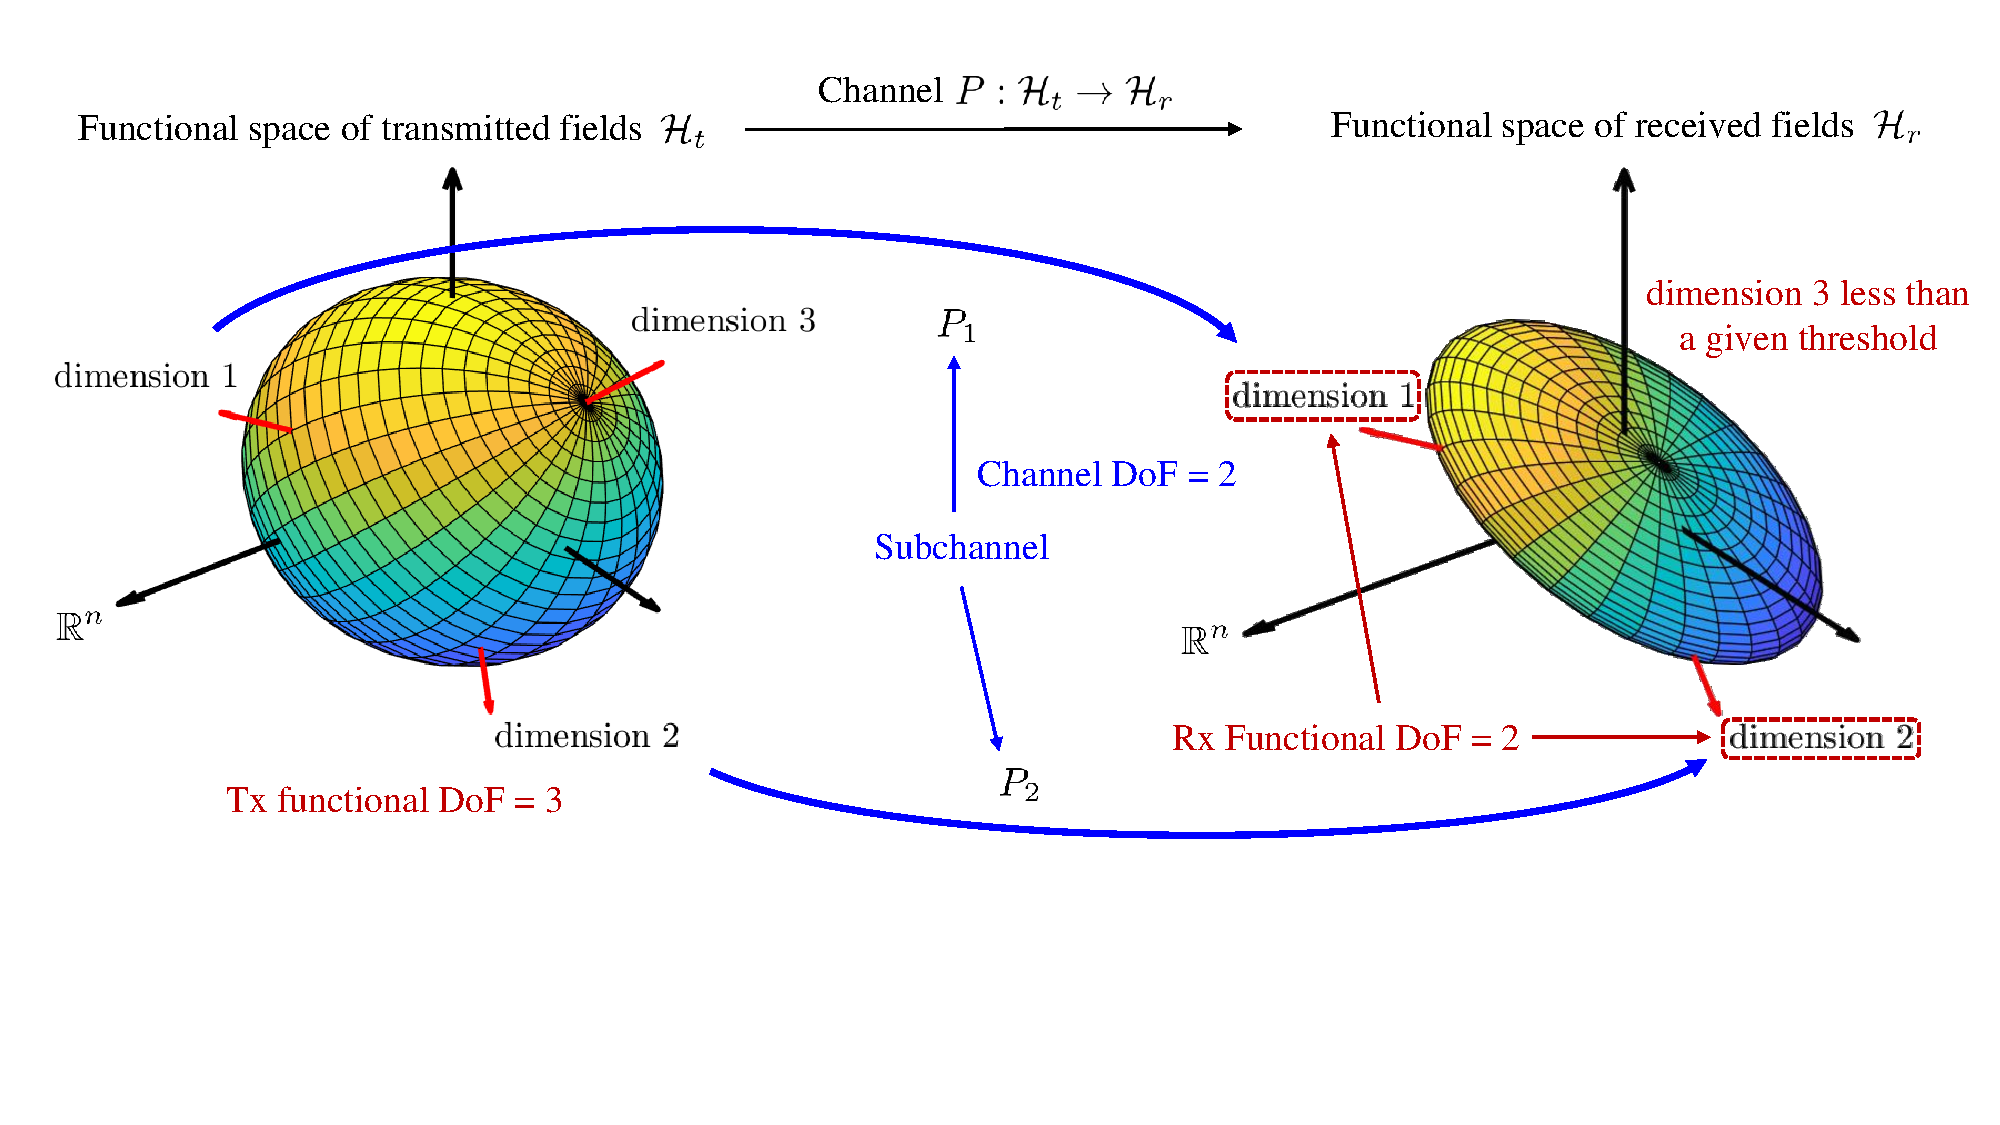
\includegraphics[width=1\textwidth]{figs/FDoFandCDoF.pdf} 
		\caption{Description of the definition of functional DoF and channel DoF.} 
		\label{FDoFandCDoF}
	\end{figure*}

\subsection{\color{red}Relationship between functional DoF and channel DoF}

\label{sec:Relationship_theorem}
	
	\begin{lemma}
		\label{lemma_CS_inequality}
		Assume that $g$ is square-integrable on $\mathcal{A} \subset \mathbb{R}^n$, the kernel function of integral operator $P$ is square-integrable on $\mathcal{A}*\mathcal{B} \subset \mathbb{R}^{n+m}$.
		We define $\left\|  g \right\|:=\sqrt{\int_{\mathcal{A}}|g({\bf x})|^2{\rm d}^n{\bf x}}$ and $\left\| P \right\|:=\sqrt{\int_{\mathcal{B}} \int_{\mathcal{A}}\Big|P({\bf x},{\bf x}')\Big|^2 {\rm d}^n{\bf x}' {\rm d}^m{\bf x} }$. Then we have $\left\| Pg  \right\| \leqslant \left\| P  \right\|\left\| g  \right\| $.
	\end{lemma}
	\begin{proof}
		For $\left\| Pg  \right\|$ we have
		\begin{equation}
			\begin{aligned}
				\left\|  Pg \right\| &= \sqrt{\int_{\mathcal{B}} \Big|\int_{\mathcal{A}}P({\bf x},{\bf x}')g({\bf x}'){\rm d}^n{\bf x}'\Big|^2{\rm d}^m{\bf x}}
				\\&\leqslant \sqrt{\int_{\mathcal{B}} \int_{\mathcal{A}}\Big|P({\bf x},{\bf x}')\Big|^2 {\rm d}^n{\bf x}' {\rm d}^m{\bf x} }
				\sqrt{\int_{\mathcal{A}}\Big|g({\bf x}')\Big|^2{\rm d}^n{\bf x}'},
			\end{aligned}
		\end{equation}
		according to Cauchy–Schwarz inequality.
	\end{proof}
	
	To intuitively show the definition of the functional DoF and channel DoF, we plot Fig. \ref{FDoFandCDoF} which includes the functional space of transmitted and received fields $\mathcal{H}_t$ and $\mathcal{H}_r$. It is shown that the functional DoF corresponds to the number of orthogonal base functions in the functional space needed to construct the space with required accuracy. Moreover, the channel DoF corresponds to the number of subchannels needed to project arbitrary function in $\mathcal{H}_t$ to a function in $\mathcal{H}_r$ with required accuracy. It is expected that the channel DoF is upper-bounded by the functional DoF of the fields at the transceivers. We provide the following theorem to rigorously prove their relationship. 
	
	\begin{theorem}
		\label{theorem_1}
		(The relationship between the functional DoF and the channel DoF) Let $\mathcal{H}_{\rm t}$ and $\mathcal{H}_{\rm r}$ be two Hilbert spaces and $P:\mathcal{H}_{\rm t} \rightarrow \mathcal{H}_{\rm r}$ be an operator. The functional DoF of $\mathcal{H}_{\rm t}$ with error $\epsilon_1$ is $N_1$. The functional DoF of $\mathcal{H}_{\rm r}$ with error $\epsilon_2$ is $N_2$. Then the channel DoF of the operator $P: \mathcal{H}_{\rm t} \rightarrow \mathcal{H}_{\rm r}$ with error $\left\| P \right\| \epsilon_1 + \left\|  P \right\| (1+\epsilon_1) \epsilon_2$ is at most ${\rm max}\{N_1,N_2\}$, i.e.,
		\begin{equation}
			\begin{aligned}
			&\mathsf{cDoF}_{\left\| P \right\| \epsilon_1 + \left\|  P \right\| (1+\epsilon_1) \epsilon_2}({\mathcal{H}_{\rm t}},{\mathcal{H}_{\rm r}},P) \leqslant {\rm max}\{\mathsf{fDoF}_{\epsilon_1}(\mathcal{H}_{\rm t}),\mathsf{fDoF}_{\epsilon_2}(\mathcal{H}_{\rm r})\}.
			\end{aligned}
		\end{equation}
	\end{theorem}
	
	\begin{proof}
		For the space $\mathcal{H}_{\rm t}$, it has DoF $N_1$ and with error $\epsilon_1$ according to the above definition. The basis on $\mathcal{H}_{\rm t}$ are defined as $g_{i=1}^{N_1}$, which constructs the subspace $\hat{\mathcal{H}}_{\rm t}$. For the space $\mathcal{H}_{\rm r}$, it has DoF $N_2$ with error $\epsilon_2$ according to the above definition. The basis on $\mathcal{H}_{\rm r}$ are defined as $f_{i=1}^{N_2}$, which constructs the subspace $\hat{\mathcal{H}}_{\rm r}$. If $N_1=N_2$, we have a set of operators $P_1^n$ that satisfies $P_ig_j=f_i {\mathbbm 1}_{i=j}$. Moreover, $\bra{P_i g}P_j g\rangle =0$ for arbitrary $g \in \hat{\mathcal{H}}_{\rm t}$ and $i \neq j$. Otherwise, if $N_1<N_2$, we add $N_2-N_1$ base functions $g_{i=N_1+1}^{N_2}$ in $\mathcal{H}_{\rm t}$, which expands $\hat{\mathcal{H}}_t$ to $\tilde{\mathcal{H}}_{\rm t}$. It is obvious that $\mathcal{H}_{\rm t}$ has DoF $N_2$ with error $\tilde{\epsilon}_1\leqslant \epsilon_1$. If $N_1>N_2$, similar operation can be done on $\mathcal{H}_{\rm r}$, showing that $\mathcal{H}_{\rm r}$ has DoF $N_1$ with error $\tilde{\epsilon}_2\leqslant \epsilon_2$.
		
		From the above analysis, we define $N_3 = {\rm max}\{N_1,N_2\}$.
		Now for arbitrary $g \in \mathcal{H}_{\rm t} $ and $\left\| g\right\|=1$, there exists a set of parameters $b_i$ that satisfies $\left\|g-\sum_{i=1}^{N_3}b_ig_i \right\| \leqslant \epsilon_1$. From \eqref{eqn_min_f_approx} we know that the minimum of $\left\|g-\sum_{i=1}^{N_3}b_ig_i\right\|$ is achieved when $b_i = \frac{ \langle g \ket{g_i}}{\left\| g_i \right\|^2}$. Then we have
		\begin{equation}
			\begin{aligned}
				\langle g-\sum_{i=1}^{N_3}b_ig_i \ket{g_j} =\langle g\ket{g_j} - b_i \langle g_i\ket{g_j}=0.
			\end{aligned}
		\end{equation}
 Then we choose $b_i$ that satisfies the above conditions. For arbitrary $P$ we have $\left\| Pg-P \sum_{i=1}^{N_3}b_ig_i \right\| \leqslant \left\| P \right\| \epsilon_1$ according to {\bf Lemma 1}. Noted that there exists $f=P\sum_{i=1}^{N_3}b_ig_i \in \mathcal{H}_{\rm r}$. Moreover, according to the definition of the DoF of space $\mathcal{H}_{\rm r}$, we have $a_{i=1}^{N_3}$ that satisfy $\left\| f-\sum_{i=1}^{N_3} a_i f_i  \right\| \leqslant \left\| f \right\| \tilde{\epsilon}_2 \leqslant \left\|  P \right\| (1+\tilde{\epsilon}_1) \tilde{\epsilon}_2$. For the rank-1 operators $P_i$ we construct them as $P_i = \frac{\ket{f_i} \bra{g_i}}{\left\| g_i^2\right\|^2}$. Then we can construct $P_1 = \sum_{i=1}^{N_3} a_i P_i/b_i$, which leads to $P_1\sum_{i=1}^{N_3}b_ig_i =\sum_{i=1}^{N_3} a_i f_i $.
		
		Based on the construction scheme of $P_1$, we have 
		\begin{equation}
			\begin{aligned}
				P_1 (g-\sum_{i=1}^{N_3}b_ig_i ) &= \sum_{j=1}^{N_3}\frac{a_j}{b_j} \ket{f_j} \bra{g_j} g-\sum_{i=1}^{N_3}b_ig_i \rangle
				 = \sum_{j=1}^{N_3}\frac{a_j}{b_j} \ket{f_j} \left(\bra{g-\sum_{i=1}^{N_3}b_ig_i} g_j \rangle \right)^* = 0.
			\end{aligned}
		\end{equation}
		
		Then, we have the following inequality
		\begin{equation}
			\begin{aligned}
				\left\|  Pg - P_1 g  \right\| &\leqslant \left\| (P-P_1)(g-\sum_{i=1}^{N_3}b_ig_i)  \right\|  + \left\| P\sum_{i=1}^{N_3}b_ig_i -P_1\sum_{i=1}^{N_3}b_ig_i  \right\|
				\\&= \left\| P(g-\sum_{i=1}^{N_3}b_ig_i)  \right\|  + \left\| f - \sum_{i=1}^{N_3} a_i f_i \right\|
				\\& \leqslant \left\| P \right\| \tilde{\epsilon}_1 + \left\|  P \right\| (1+\tilde{\epsilon}_1) \tilde{\epsilon}_2
				\\&\leqslant \left\| P \right\| \epsilon_1 + \left\|  P \right\| (1+\epsilon_1) \epsilon_2.
			\end{aligned}
		\end{equation}
		
			Therefore, we can conclude that the channel DoF is no more than ${\rm max}\{N_1,N_2\}$ with error $\left\| P \right\| \epsilon_1 + \left\|  P \right\| (1+\epsilon_1) \epsilon_2$.
	\end{proof}
	
	\begin{remark}
		Through {\bf Theorem 2} we provide the relationship between functional DoF and channel DoF, showing that the channel DoF is upper-bounded by the functional DoF at the transceivers. Here it is worth noting that the bound is a weak bound while a tight bound related to ${\rm min}\{N_1,N_2\}$ is expected inspired by classical discrete MIMO theory, which remains for further works.
	\end{remark}

	{\color{red}
	\begin{remark}
		In {\bf Theorem 2} we provide an upperbound of cDoF using fDoF. While a lowerbound will further strengthen the work, it highly relies on the characteristics of the channel operator $P$. Now we will show the reason. We assume that each function in $\mathcal{H}_{\rm r}$ has a preimage in $\mathcal{H}_{\rm t}$ through the projection $P$. According to the definition of fDoF in $\mathcal{H}_{\rm r}$ we know that there exists a function $f\in \mathcal{H}_{\rm r}$ with modulus 1 that at least $n$ bases should be used to represent it with error $\epsilon_2$. Let $Pg = f$ and $\left\| g\right\| = a$, we know that the channel DoF with error $\epsilon_2/a$ should be no less than $fDoF_{\epsilon_2}(\mathcal{H}_r)$. From {\bf Lemma} \ref{lemma_CS_inequality} we know that $a \geqslant 1/\left\|  P \right\|$ but can not know the upperbound of $a$, which relies on $P$ and determines the lower bound of cDoF. If we denote the upperbound of $a$ by $a_0$, it is obvious that $cDoF_{a_0\epsilon_2}(\mathcal{H}_t,\mathcal{H}_r,P)\geqslant fDoF_{\epsilon_2}(\mathcal{H}_r)$. 
	
	\end{remark}
	}

	{\color{red}\subsection{Relationship between DoF, mutual information and capacity for EIT}
	
	In the previous part, we have provided mathematical definitions about the functional DoF of electromagnetic fields (fDoF) and the channel DoF which further considers channel conditions between the transceivers (cDoF). Moreover, we have provided the analysis of the relationship between fDoF and cDoF. In this part, we will have some discussions about the relationship between the defined DoF and other concepts like mutual information and capacity, which have already been widely discussed in the research field of EIT.

	As shown in Sec. \ref{sec:Relationship_theorem}, the proposed fDoF provides an upperbound for all kinds of channel conditions. Therefore, we can design the deployment strategies of transceivers based on the obtained fDoF, which has the maximum redundancy. To be more specific, no matter how the channel condition changes, the designed system can capture all the possible DoF in the system. The relationship between fDoF and cDoF is explained in {\bf Theorem} \ref{theorem_1}. When considering a specific channel, cDoF can be used and has a deep connection to the mutual information and capacity. In \cite{wan2022mutual} we have expressed the mutual information between random electromagnetic fields as $I(E;Y) = \sum_i{\rm log}(1+\frac{\lambda_i}{\sigma^2})$ based on Mercer' s theorem \cite{mercer1909xvi}. It can be observed that the mutual information can be expressed as the summation of infinite terms derived from the statistical characteristics of the received fields, which are determined by the channel. Each item in the expression of mutual information corresponds to one degree of freedom, where different $\lambda$ reflecting the criticality weight of the corresponding sub-channel, as discussed in Definition \ref{def_cDoF}.

	When further considering channel capacity, we shall fix the field distribution which maximizes the mutual information to obtain the capacity based on continuous electromagnetic fields and channels. This procedure is an extension from the discrete matrices to continuous operators, represented as $P$ in Definition \ref{def_cDoF}. For discrete matrices we have $C = \underset{K_J}{\rm max}{\rm logdet}\frac{HK_JH^{\rm H}+K_N}{K_N}$ with respect to ${\rm Tr}(K_J) \leqslant P$. By using singular value decomposition and Karush–Kuhn–Tucker (KKT) theorem, we can obtain the maximum mutual information which is the capacity. For operators, the optimization problem can be solved by the extended KKT theorem \cite{bachir2021finitely} for countably infinite variables. The result is in the form of the water-filling method, where the insignificant subchannels are discarded, leaving only the channels corresponding to large eigenvalues. This procedure is the same as what we have done in the definition of DoF. 

	In all, the proposed fDoF has and indirect relation with mutual information and capacity, which is established by cDoF. Besides, all these concepts used in EIT are based on continuous electromagnetic fields which are in spaces with infinite dimensions. This property, distinct from finite-dimensional matrices, entails the necessity of filtering out insignificant basis functions or subchannels based on the error tolerance threshold $\epsilon$. 
	
	}
	
	\section{DoF analysis based on Slepian concentration problem}
	\label{sec_theoretical_dof}
	In this part, we will discuss the DoF of electromagnetic fields using the theoretical tools from the Slepian concentration problem. 
	Slepian concentration problem considers the optimal representation of a signal bandlimited in the frequency domain and approximately bandlimited in the time domain by using a set of orthogonal bases. The number of the base functions that need to be used to approximate the signal with a given error threshold represents the DoF of the signal space that satisfies the above conditions. {\color{red}We will first introduce existing works about the Slepian concentration problems in the literature and the difference in our work. Then we will show the mathematical forms of the Slepian concentration problem in one and two-dimensional cases, which have been discussed in the literature. By considering electromagnetic constraints, we extend the Slepian concentration problem to the three-dimensional space domain and four-dimensional space-time domain, and provide some discussions about the properties of eigenvalues and eigenfunctions solved from the Slepian concentration problem}. 

	{\color{red}
	\subsection{A brief introduction of the existing works on Slepian concentration problem}
	}
	
	{\color{red}
	The original work, accomplished by Slepian, analyzed the one-dimensional time-frequency concentration problem which has analytical solutions for the eigenvalues and eigenfunctions\cite{slepian1961prolate}. Based on these analytical solutions, the number of large eigenvalues and the behavior of the decay rate of small eigenvalues can be directly analyzed. The results about the one-dimensional Slepian concentration problem serve as powerful tools, which have been widely adopted in many areas, including spectrum estimation\cite{thomson2005spectrum}, capacity analysis\cite{cover1999elements}, numerical integration\cite{xiao2001prolate}, uncertainty relations\cite{furrer2014position}, etc.
	
	Slepian has also discussed the possible extension of the concentration problem to high dimensions with sphere-shaped concentration region\cite{slepian1964prolate}, but provided no analytical solutions for the eigenvalues. Many researchers have followed his work, analyzing the Slepian concentration problem with different domain representations and concentration regions. Due to the high complexity of the high-dimensional structures, even for highly symmetric models, the existing works still focus on numerical calculation schemes instead of finding analytical solutions for the eigenvalue and eigenfunction solutions. 

	For the domain representation, one approach is constraining one domain on a sphere and the other domain using degrees and orders of spherical harmonic functions. An early work considering both asymptotic results and numerical calculations in non-asymptotic scenarios has been discussed in \cite{simons2006spatiospectral}. Further works added colatitude–longitude spatial region constraints on the sphere and provided numerical calculation schemes for the eigen-problem \cite{bates2016slepian}. Since our DoF analysis is with the physical constraints in space-wavenumber domains, the constraints based on spherical harmonic functions do not well fit our needs. 
	
	Another approach is directly considering two domains that are the Fourier transform or the inverse Fourier transform of each other. By directly performing sampling on the constraint regions, \cite{beylkin2007grids} considered the two-dimensional Slepian concentration problem with a disc-shaped constraint region in one domain and a rectangle-shaped region in the other domain. In a similar form, \cite{simons2011spatiospectral} considered disc-shaped constraint regions in both two domains. 
	The fast-converging numerical calculation scheme for evaluating the two-dimensional Slepian concentration problem was analyzed in \cite{shkolnisky2007prolate}, which considered disc-shaped constraints in two domains that are Fourier transform or inverse Fourier transform of each other. 
	Its further extension to higher dimensional balls was shown in \cite{zhang2020ball}, which also considered numerical schemes and had no analytical solutions. Moreover, these two papers considered an ideal case when the concentration regions in the two domains are both $n$-dimensional balls, while our concentration region in the space domain may not always have spherical symmetry. 

	Compared to these existing mathematical works, in this paper, we will formulate the Slepian concentration problem in the three-dimensional space-wavenumber domain and the four-dimensional domain which also includes time-frequency. We will obtain the concentration region in the wavenumber domain based on physical constraints like the dispersion relation. How to integrate physical constraints with the concentration problem is the main challenge and the focus of the following parts in this section. In particular, in the case of single-frequency points, which is the focus of many recent papers \cite{gong2023holographic,wei2023tri, pizzo2023wide}, the subsequent analysis will show that the asymptotic conclusions completely lose their validity. Compared to spherical regions, we mainly focus on a cuboid-shaped spatial concentration region that fits transceivers in reality better, which will break the spherical symmetry and make performing theoretical analysis even harder.  
	
	In all, we can find that providing analytical solutions for the eigenvalues and eigenfunctions when considering the Slepian concentration problem in high dimensions is very difficult. Therefore, obtaining numerical solutions after deriving the integral equations, which is not the best but is a practically feasible route, is chosen in our paper. Besides numerical simulations, we also provide some quantitative and qualitative analyses and discussions of the properties of the eigenvalues based on the derived kernel functions, which will be shown in the following parts.

}
	
	\subsection{Slepian concentration problem in one and two-dimensional domain}
	\label{subsec_1d2d_Selpian}
	For typical one-dimensional time and frequency domain, the Slepian concentration problem is formulated in the following part.
	We have the one-dimensional Fourier transform and inverse Fourier transform
	\begin{equation}
		\begin{aligned}
			f(t) = (2\pi)^{-1}\int_{-\infty}^{+\infty}F(\omega)e^{{\rm j}\omega t}{\rm d}\omega,
		\end{aligned}
	\end{equation}
	and
	\begin{equation}
		\begin{aligned}
			F(\omega) = \int_{-\infty}^{+\infty}f(t)e^{-{\rm j}\omega t}{\rm d}t.
		\end{aligned}
	\end{equation}
	Then for a bandlimited signal $G(\omega) = \int_{-T}^{+T}g(t)e^{-{\rm j}\omega t}{\rm d}t$, the optimally concentrated signal is taken to be the one that maximizes $\lambda = \frac{\int_{-\Omega}^{\Omega}|G(\omega)|^2{\rm d}\omega}{\int_{-\infty}^{\infty}|G(\omega)|^2{\rm d}\omega}$, which leads to the following integral equation
	\begin{equation}
	\begin{aligned}
		\int_{-T}^{T}D(t,t'){\color{red}g_i}(t'){\rm d}t' = {\color{red}\lambda_{i} g_i(t)},
	\end{aligned}
	\label{eqn_1d_t}
	\end{equation}
	and
	\begin{equation}
		\begin{aligned}
			D(t,t') = (2\pi)^{-1}\int_{-\Omega}^\Omega e^{{\rm j}\omega(t-t')}{\rm d}\omega = \frac{\sin(\Omega(t-t'))}{\pi(t-t')}.
		\end{aligned}
	\end{equation}
	By analyzing the asymptotic behavior of the eigenvalue $\lambda$, it is known that the dimension of the signal space is asymptotically
	\begin{equation}
		\begin{aligned}
			N^{1D} = \sum_{i=1}^\infty \lambda_i = \int_{-T}^{T}D(t,t){\rm d}t = \frac{2\Omega T}{\pi},
		\end{aligned}
	\end{equation}
	when $\Omega T \rightarrow \infty$ \cite{slepian1961prolate}. We show in Fig. \ref{1d_omegaT} that when $\Omega T \rightarrow \infty$, the decay line of eigenvalues will have a cut-off transition. {\color{red} Here we use numerical schemes to solve the integral equation (\ref{eqn_1d_t}) to obtain Fig. \ref{1d_omegaT}. Specifically, we substitute $\int$ by $\sum$ in (\ref{eqn_1d_t}) and solve the corresponding eigen-problem of matrix generated by $D(t,t')$. Since in the one-dimensional case the solutions for (\ref{eqn_1d_t}) has analytical forms \cite{slepian1961prolate}, directly using these solutions can also obtain the same result.} Nearly $N^{1D}$ eigenvalues are on the left side of the transition line, which tend to the same maximum value. Moreover, nearly all eigenvalues on the right side of the transition line tends to 0. Therefore, $N^{1D}$ is the asymptotic DoF of the signal space when $\Omega T \rightarrow \infty$. {\color{red}It is worth noting that we can find the ``optimally concentrated signal" both from time and frequency domains, and the eigenvalue $\lambda$ will be the same. When beginning from $g(t) = (2\pi)^{-1}\int_{-\Omega}^{\Omega}G(\omega)e^{{\rm j}\omega t} {\rm d}\omega$, we have $\lambda = \frac{\int_{-T}^{T}|g(t)|^2{\rm d}t}{\int_{-\infty}^{\infty}|g(t)|^2{\rm d}t}$. Then we have 
	\begin{equation}
	\begin{aligned}
		\int_{-\Omega}^{\Omega}D(\omega,\omega')G_i(\omega'){\rm d}\omega' = \lambda_i G_i(\omega),
	\end{aligned}
	\label{eqn_1d_omega}
	\end{equation}
	and
	\begin{equation}
		\begin{aligned}
			D(\omega,\omega') = (2\pi)^{-1}\int_{-T}^T e^{-{\rm j}t(\omega-\omega')}{\rm d}t = \frac{\sin(T(\omega-\omega'))}{\pi(\omega-\omega')}.
		\end{aligned}
	\end{equation}
	It is easy to verify that the eigenvalues in (\ref{eqn_1d_t}) and (\ref{eqn_1d_omega}) are the same.
	}
	
	\begin{figure}
		\centering 
		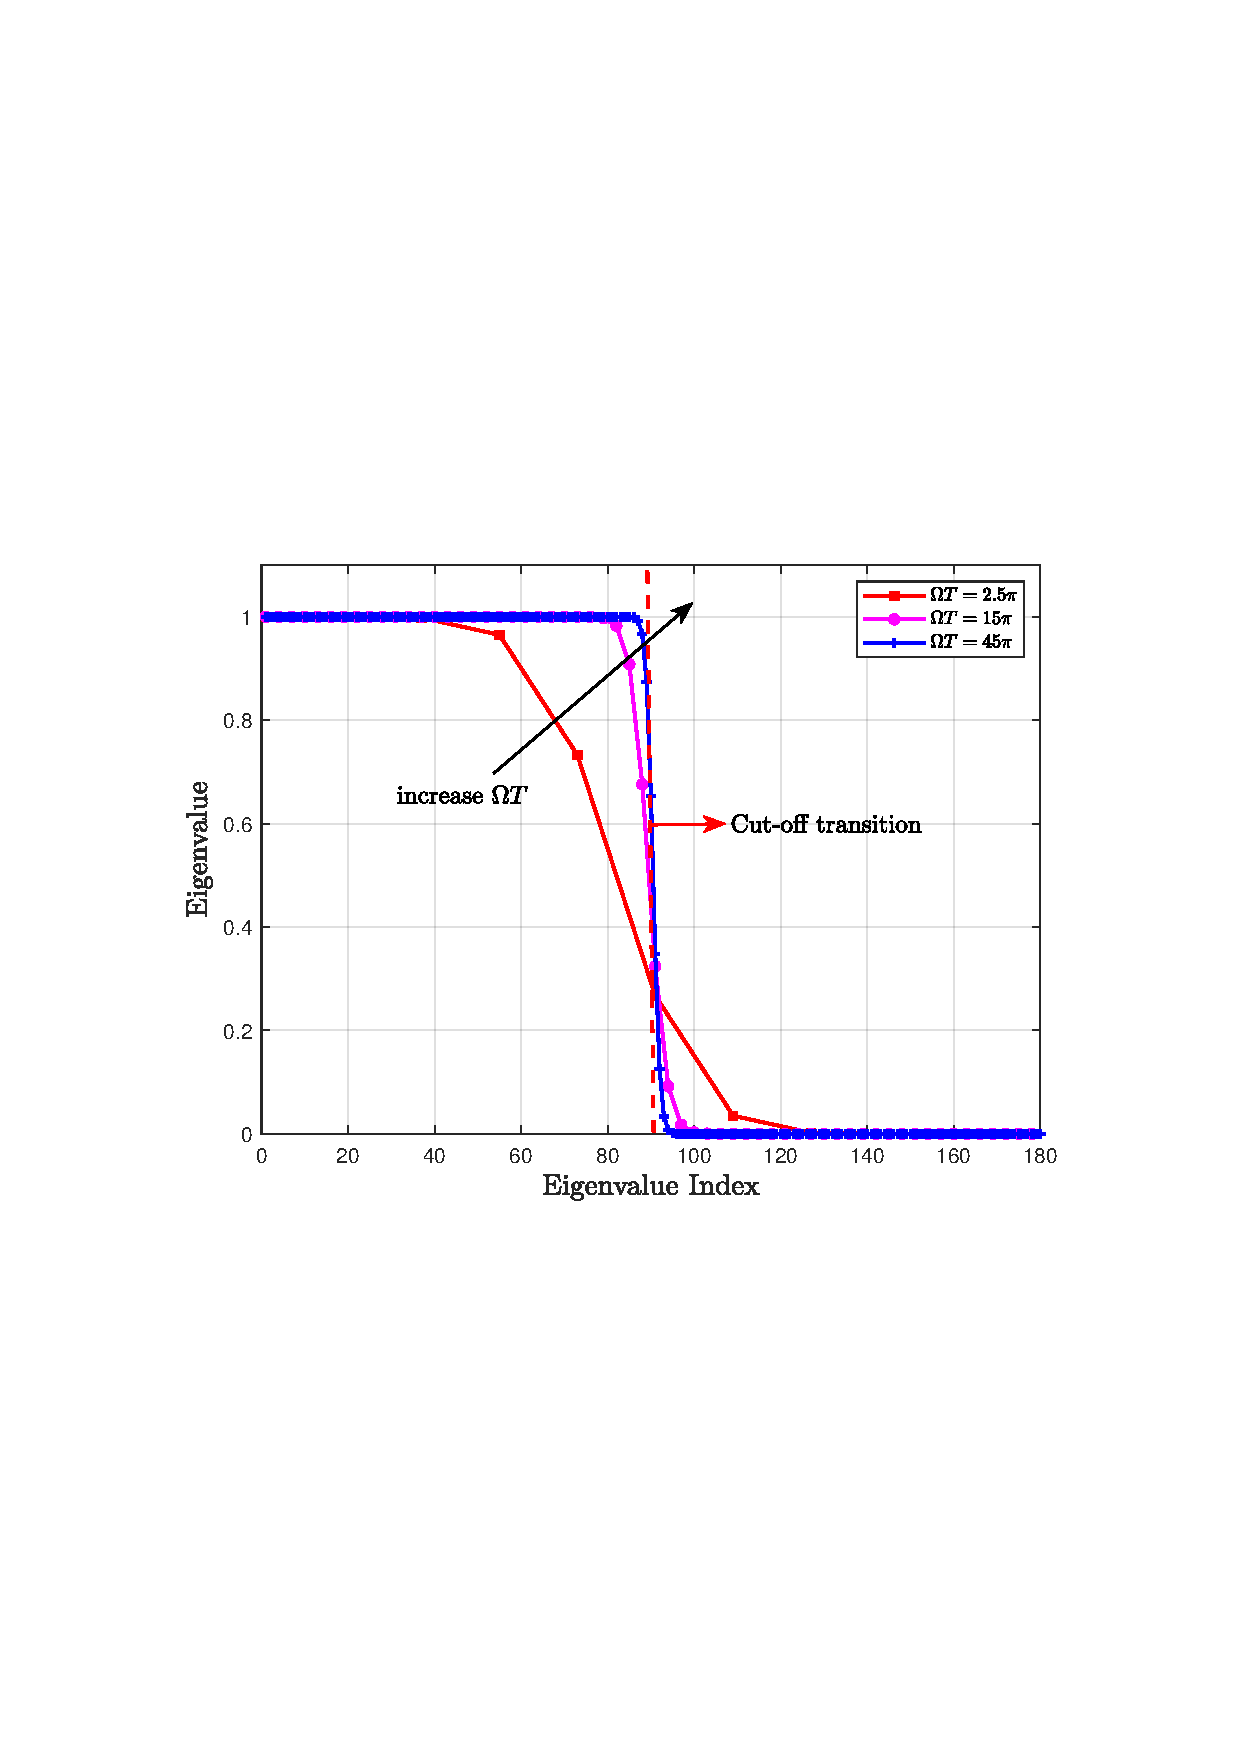
\includegraphics[width=0.7\textwidth]{figs/save_1d_different_omegaT.pdf} 
		\caption{The eigenvalues of one-dimensional Slepian concentration problem when $\Omega T$ increases.} 
		\label{1d_omegaT}
	\end{figure}
	
	For two-dimensional case, similar problem is formulated in the literature as follows:
	\begin{equation}
		\begin{aligned}
			f({\bf x})=(2\pi)^{-2}\int_{-\infty}^{+\infty}F({\bf k})e^{{\rm j}{\bf k}\cdot {\bf x}}{\rm d}^2{\bf k},
		\end{aligned}
		\label{eq_2d_fourier}
	\end{equation}
	and
	\begin{equation}
		\begin{aligned}
			F({\bf k}) = \int_{-\infty}^{+\infty}f({\bf x})e^{-{\rm j}{\bf k}\cdot {\bf x}}{\rm d}^2{\bf x}.
		\end{aligned}
	\end{equation}
	{\color{red} The concentration regions in the two domains are represented as $\mathcal{R}$ and ${\mathcal{K}}$.} The integral equation corresponding to the two-dimensional eigenfunctions and eigenvalues is 
	\begin{equation}
		\begin{aligned}
			\int_{\mathcal{R}}D({\bf x},{\bf x}'){\color{red}f_i({\bf x}')}{\rm d}^2{\bf x}' = {\color{red}\lambda_i f_i({\bf x})},
		\end{aligned}
		\label{eqn_2d_integral}
	\end{equation}
	and
	\begin{equation}
		\begin{aligned}
			D({\bf x},{\bf x}') &= (2\pi)^{-2}\int_{\mathcal{K}} e^{{\rm j}{\bf k}\cdot({\bf x}-{\bf x}')}{\rm d}^2{\bf k} = \frac{K}{2\pi} \frac{J_1(K\left\| {\bf x}-{\bf x}' \right\|)}{\left\| {\bf x}-{\bf x}' \right\|},
		\end{aligned}
	\end{equation}
	where $\mathcal{K} = \{{\bf k} : \left\| {\bf k} \right\|\leqslant K\}$ is disk-shaped \cite{beylkin2007grids}. 
	The DoF when $K^2A \rightarrow \infty$ is 
	\begin{equation}
		\begin{aligned}
			N^{2D} = \sum_{i=1}^\infty \lambda_i = \int_{\mathcal{R}}D({\bf x},{\bf x}){\rm d}^2{\bf x} = \frac{K^2A}{4\pi},
		\end{aligned}
		\label{eq_2d_dof}
	\end{equation}
	where $A$ is the area of $\mathcal{R}$. 
	
	\subsection{Slepian concentration problem in three-dimensional space-wavenumber domain for electromagnetic field}
	\label{subsec_3d_slepian}
	
	Now we will analyze the case with three-dimensional domain, which depicts the electromagnetic fields in the space. We consider the constraints of electromagnetic fields in space and wavenumber domain. In space domain the electromagnetic field is observed within the region of transceivers. In wavenumber domain the electromagnetic field is constrained by the frequency settings according to dispersion relation. There are two different cases of the constraints in wavenumber domain. The first one is with a frequency bandwidth, which corresponds to the constraint region as a ball in the wavenumber domain ($k_x^2+k_y^2+k_z^2 \leqslant k_0^2$) or a spherical shell in the wavenumber domain ($k_1^2 \leqslant k_x^2+k_y^2+k_z^2 \leqslant k_0^2$). The second one is on a single-frequency point, which corresponds to the constraint region as a sphere in the wavenumber domain ($k_x^2+k_y^2+k_z^2=k_0^2$). {\color{red} We denote the concentration region in the space domain as $\mathcal{R}$, and the concentration region in the wavenumber domain as $\mathcal{K}$.} For the first case similar to what has been discussed in one-dimensional and two-dimensional examples, we have 
	\begin{equation}
		\begin{aligned}
			f({\bf x})=(2\pi)^{-3}\int_{-\infty}^{+\infty}F({\bf k})e^{{\rm j}{\bf k}\cdot {\bf x}}{\rm d}^3{\bf k},
		\end{aligned}
	\end{equation}
	and
	\begin{equation}
		\begin{aligned}
			F({\bf k}) = \int_{-\infty}^{+\infty}f({\bf x})e^{-{\rm j}{\bf k}\cdot {\bf x}}{\rm d}^3{\bf x}.
		\end{aligned}
	\end{equation}
	If the wavenumber domain constraint satisfies $k_x^2+k_y^2+k_z^2 \leqslant k_0^2$, we have 
	\begin{equation}
		\begin{aligned}
			D({\bf x},{\bf x}') &= (2\pi)^{-3}\int_{\mathcal{K}} e^{{\rm j}{\bf k}\cdot({\bf x}-{\bf x}')}{\rm d}^3{\bf k} \\&= (2\pi)^{-3} \int_{0}^{k_0} \int_{{\Omega}=\{\hat{\bf k}: \left\| \hat{\bf k} \right\|=1\}} e^{{\rm j}k\hat{\bf k}\cdot({\bf x}-{\bf x}')}k^2{\rm d}^2S{\rm d}k
			\\& = (2\pi)^{-3} 4\pi \int_0^{k_0} \frac{\sin k \left\| {\bf x}-{\bf x}' \right\|}{k \left\| {\bf x}-{\bf x}' \right\|}k^2 {\rm d}k
			\\& = \frac{1}{2\pi^2} \left( \frac{\sin k\left\| {\bf x}-{\bf x}' \right\|}{\left\| {\bf x}-{\bf x}' \right\|^3}-\frac{k\cos k\left\| {\bf x}-{\bf x}' \right\|}{\left\| {\bf x}-{\bf x}' \right\|^2} \right) \Bigg|_0^{k_0}
			\\& = \frac{1}{2\pi^2} \left( \frac{\sin k_0\left\| {\bf x}-{\bf x}' \right\|}{\left\| {\bf x}-{\bf x}' \right\|^3}-\frac{k_0\cos k_0\left\| {\bf x}-{\bf x}' \right\|}{\left\| {\bf x}-{\bf x}' \right\|^2} \right).
		\end{aligned}
		\label{equ_ball}
	\end{equation}
	The asymptotic DoF is 
	\begin{equation}
		\begin{aligned}
			N^{3D} = \sum_{i=1}^\infty \lambda_i = \int_{\mathcal{R}}D({\bf x},{\bf x}){\rm d}^3{\bf x} = \frac{V}{6\pi^2}k_0^3,
		\end{aligned}
	\end{equation}
	{\color{red} where $V$ is the volume of $\mathcal{R}$.}
	
	If the wavenumber domain constraint satisfies $k_1^2\leqslant k_x^2+k_y^2+k_z^2 \leqslant k_0^2$, similarly we have
	\begin{equation}
		\begin{aligned}
			D({\bf x},{\bf x}') =& \frac{1}{2\pi^2} \left( \frac{\sin k_0\left\| {\bf x}-{\bf x}' \right\|}{\left\| {\bf x}-{\bf x}' \right\|^3}-\frac{k_0\cos k_0\left\| {\bf x}-{\bf x}' \right\|}{\left\| {\bf x}-{\bf x}' \right\|^2} \right)
	-\frac{1}{2\pi^2} \left( \frac{\sin k_1\left\| {\bf x}-{\bf x}' \right\|}{\left\| {\bf x}-{\bf x}' \right\|^3}-\frac{k_1\cos k_1\left\| {\bf x}-{\bf x}' \right\|}{\left\| {\bf x}-{\bf x}' \right\|^2} \right).
		\end{aligned}
		\label{equ_spherical_shell}
	\end{equation}
	The asymptotic DoF is 
	\begin{equation}
	\begin{aligned}
		N^{3D} = \sum_{i=1}^\infty \lambda_i = \int_{\mathcal{R}}D({\bf x},{\bf x}){\rm d}^3{\bf x} = \frac{V}{6\pi^2}(k_0^3-k_1^3).
	\end{aligned}
	\end{equation}
	\begin{remark}
		Here the asymptotic DoF is achieved when $V(k_0^3-k_1^3)$ tends to infinity. For the single-frequency point where $k_0=k_1$, the asymptotic DoF becomes 0, which seems no longer correct. We will do further discussion on it in the following part. 
		\end{remark}
	
%	For the single-frequency point case, a delta function $\delta(k-k_0)$ need to be introduced to concentrate the function on the sphere in wavenumber domain. We denote $F({\bf k}) = F_1(\theta,\phi)\delta(k-k_0)$
%	
%		\begin{equation}
%		\begin{aligned}
%			f({\bf x})=(2\pi)^{-3}\int_{{\Omega}=\{\hat{\bf k}: \left\| \hat{\bf k} \right\|=1\}}k_0^2F_1(\theta,\phi)e^{{\rm j}k_0\hat{\bf k}\cdot {\bf x}}{\rm d}S,
%		\end{aligned}
%	\end{equation}
%	\begin{equation}
%		\begin{aligned}
%			F({\bf k}) = \int_{-\infty}^{+\infty}f({\bf x})e^{-{\rm j}{\bf k}\cdot {\bf x}}{\rm d}{\bf x},
%		\end{aligned}
%	\end{equation}
%	and
%	\begin{equation}
%		\begin{aligned}
%			F_1(\theta,\phi) &= 
%			\int_{0}^{\infty} \int_{-\infty}^{+\infty}f({\bf x})e^{-{\rm j}{\bf k}\cdot {\bf x}}{\rm d}{\bf x} {\rm d}k
%		\end{aligned}
%	\end{equation}
%	
%	Then similar to the previous cases, we have 
%	\begin{equation}
%		\begin{aligned}
%			D({\bf x},{\bf x}') &= (2\pi)^{-3}\int_{{\Omega}=\{\hat{\bf k}: \left\| \hat{\bf k} \right\|=1\}}k_0^2e^{{\rm j}k_0\hat{\bf k}\cdot {\bf x}}{\rm d}S
%			\\& = \frac{1}{2\pi^2} \frac{k_0\sin k_0 \left\| {\bf x}-{\bf x}' \right\|}{\left\|  {\bf x}-{\bf x}' \right\|}.
%			\end{aligned}
%		\end{equation}
%	The DoF accordingly is 
%		\begin{equation}
%		\begin{aligned}
%			N^{3D} = \sum_{i=1}^\infty \lambda_i = \int_{\mathcal{R}}D({\bf x},{\bf x}){\rm d}{\bf x} = \frac{V}{2\pi^2}k_0^2.
%		\end{aligned}
%	\end{equation}
	
	For the single-frequency point case, we will use a function which converges to delta function in the $k$ axis to approach the sphere surface in wavenumber domain. We set $F({\bf k}) =F_1(\theta,\phi)F_2(k)$, where $\int_{0}^\infty F_2(k) {\rm d}k = 1$, then we have
	
	\begin{equation}
		\begin{aligned}
			f({\bf x})=&(2\pi)^{-3}\int_{{\Omega}=\{\hat{\bf k}: \left\| \hat{\bf k} \right\|=1\}}\int_{0}^{\infty}F_2(k)k^2F_1(\theta,\phi)e^{{\rm j}k\hat{\bf k}\cdot {\bf x}}{\rm d}k{\rm d}^2S,
		\end{aligned}
	\end{equation}
	and
	\begin{equation}
		\begin{aligned}
			F_1(\theta,\phi) &= 
			\frac{1}{F_2(k)} \int_{-\infty}^{+\infty}f({\bf x})e^{-{\rm j}{\bf k}\cdot {\bf x}}{\rm d}^3{\bf x}.
		\end{aligned}
	\end{equation}
	Then the kernel is represented by 
	\begin{equation}
		\begin{aligned}
			D({\bf x},{\bf x}') &= (2\pi)^{-3}\int_{{\Omega}=\{\hat{\bf k}: \left\| \hat{\bf k} \right\|=1\}}\int_{0}^{\infty}F_2(k)k^2e^{{\rm j}k\hat{\bf k}\cdot {\bf x}}{\rm d}k{\rm d}^2S.
		\end{aligned}
	\end{equation}
	The eigenvalues comes from the following integral equation
	\begin{equation}
		\lambda_i f_i({\bf x}) = \int_{\mathcal{R}}D({\bf x},{\bf x}')f_i({\bf x}'){\rm d}^3{\bf x}'.
		\label{eigenfunction_3d}
	\end{equation}
	Here we set $\{F_{2,n}(k)\}_{n=1}^{+\infty} = \frac{1}{2h}\left( 1-\frac{|k-k_0|}{2h} \right), |k-k_0|\leqslant 2h$, $h = \frac{1}{2^n}$ to be a set of functions that make $F({\bf k})$ focus on a sphere surface in the wavenumber domain. When $n \rightarrow \infty$, $F_2(k) \rightarrow \delta(k-k_0)$. {\color{red} In a more rigorous description, we have $\underset{n \rightarrow +\infty}{\rm lim}{\int_{\mathbb{R}} F_2(k)f(k) } = f(k_0)$ for arbitrary smooth and compactly supported function $f(k) \in C_c^{\infty}({\mathbb R})$. It is worth noting that we use the function series $\{F_{2,n}(k)\}_{n=1}^{+\infty}$ due to two reasons. Firstly, we can establish the connection between the case where the support in the wavenumber domain has a continuous extent in $k$ (finite n), and the case localized only at the point $k_0$ ($n \rightarrow \infty$). Secondly, we can avoid directly using delta functions since they are not genuine functions but generalized functions, which possess some properties that can not be achieved by real-valued functions. Using a series of well-defined integrable functions, known as approximate identities, to approach the delta function is a common way used in existing literature \cite{strichartz2003guide}. From the above discussions, we can also observe that the functions $\{F_{2,n}(k)\}_{n=1}^{+\infty}$ can not be arbitrarily chosen. They should satisfy the power constraint $\int F_2(k) {\rm d}k = 1$ and describe a unit point mass at $k = k_0$ when $n \rightarrow \infty$ (or can be equivalently described as "support set shrinks to 0 when $n \rightarrow \infty$")
	from the limitation perspective
	\cite{wheeler1997simplified}. 
	Then they all have the property $\underset{n \rightarrow +\infty}{\rm lim}{\int_{\mathbb{R}} F_2(k)f(k) } = f(k_0)$. There are infinite choices for such function series, but they have the same limitation as the delta function \cite{wheeler1997simplified} and will lead to the same DoF.} 
	
	To be clearer, we begin from our chosen function series, which has the following indefinite integral
	 \begin{equation}
	 	\begin{aligned}
	 		&\int\frac{1}{2h}\left( 1-\frac{|k-k_0|}{2h} \right)k^2e^{{\rm j}k\hat{\bf k}\cdot {\bf x}}{\rm d}k
	 		= \left\{\begin{matrix}
	 		g_1(k)	& k \in [k_0,k_0+2h),\\
	 			g_2(k)	& k \in (k_0-2h,k_0),
	 		\end{matrix}\right.
	 	\end{aligned}
	 \end{equation}
	 where
	 \begin{equation}
	 	\begin{aligned}
	 		g_1(k) =& -\frac{1}{4 h^2 (\hat{\bf k}\cdot {\bf x})^4}e^{{\rm j} (\hat{\bf k}\cdot {\bf x}) k} \Bigg(2 {\rm j} h (\hat{\bf k}\cdot {\bf x}) \Big(k^2 (\hat{\bf k}\cdot {\bf x})^2+2 {\rm j} k (\hat{\bf k}\cdot {\bf x})-2\Big)+{\rm j} k^3 (\hat{\bf k}\cdot {\bf x})^2 (k_0-k)\\&+(\hat{\bf k}\cdot {\bf x})^2 k (3 k-2 k_0)+2 {\rm j} (\hat{\bf k}\cdot {\bf x}) (3 k-k_0)-6\Bigg),
		 \end{aligned}
     \end{equation}
     and
    \begin{equation}
    	\begin{aligned}
    		g_2(k) =& \frac{1}{4 h^2 (\hat{\bf k}\cdot {\bf x})^4}e^{{\rm j} (\hat{\bf k}\cdot {\bf x}) k} \Bigg(-2 {\rm j} h (\hat{\bf k}\cdot {\bf x}) \Big(k^2 (\hat{\bf k}\cdot {\bf x})^2+2 {\rm j} k (\hat{\bf k}\cdot {\bf x})-2\Big)+{\rm j} k^3 (\hat{\bf k}\cdot {\bf x})^2 (k_0-k)\\&+(\hat{\bf k}\cdot {\bf x})^2 k (3 k-2 k_0)+2 {\rm j} (\hat{\bf k}\cdot {\bf x}) (3 k-k_0)-6\Bigg).
    	\end{aligned}
    \end{equation} 
    Therefore, we know that 
    \begin{equation}
    	\begin{aligned}
    		\int_{k_0-2h}^{k_0+2h} \frac{1}{2h}\left( 1-\frac{|k-k_0|}{2h} \right)k^2e^{{\rm j}k\hat{\bf k}\cdot {\bf x}}{\rm d}k
    		=& -\frac{1}{4 h^2 (\hat{\bf k}\cdot {\bf x})^4}e^{{\rm j} (\hat{\bf k}\cdot {\bf x}) k_0-2 {\rm j} h (\hat{\bf k}\cdot {\bf x})} 
    		\Bigg(e^{4 {\rm j} h (\hat{\bf k}\cdot {\bf x})} \Big(4 h^2 (\hat{\bf k}\cdot {\bf x})^2+\\&4 h (\hat{\bf k}\cdot {\bf x}) ((\hat{\bf k}\cdot {\bf x}) k_0+2 {\rm j})+(\hat{\bf k}\cdot {\bf x})^2 k_0^2+4 {\rm j} (\hat{\bf k}\cdot {\bf x}) k_0-6\Big)
    		\\&+4 h^2 (\hat{\bf k}\cdot {\bf x})^2-2 e^{2 {\rm j} h (\hat{\bf k}\cdot {\bf x})} \Big((\hat{\bf k}\cdot {\bf x})^2 k_0^2+4 {\rm j} (\hat{\bf k}\cdot {\bf x}) k_0-6\Big)\\&-4 h (\hat{\bf k}\cdot {\bf x}) ((\hat{\bf k}\cdot {\bf x}) k_0+2 {\rm j})+(\hat{\bf k}\cdot {\bf x})^2 k_0^2+4 {\rm j} (\hat{\bf k}\cdot {\bf x}) k_0-6\Bigg).
    	\end{aligned}
    \end{equation}
    When we let $h\rightarrow 0$, $\int_{k_0-2h}^{k_0+2h} \frac{1}{2h}\left( 1-\frac{|k-k_0|}{2h} \right)k^2e^{{\rm j}k\hat{\bf k}\cdot {\bf x}}{\rm d}k \rightarrow k_0^2 e^{{\rm j}k_0 \hat{\bf k}\cdot {\bf x}}$, which makes the kernel function as 
    \begin{equation}
    	\begin{aligned}
    		D({\bf x},{\bf x}') =&  \frac{1}{2\pi^2} \frac{k_0\sin k_0 \left\| {\bf x}-{\bf x}' \right\|}{\left\|  {\bf x}-{\bf x}' \right\|}.
    	\end{aligned}
		\label{eqn_spherical_surface}
    \end{equation}
    Then the integral equation transforms to
    	\begin{equation}
    	\lambda_i f_i({\bf x}) = \int_{\mathcal{R}} \frac{1}{2\pi^2} \frac{k_0\sin k_0 \left\| {\bf x}-{\bf x}' \right\|}{\left\|  {\bf x}-{\bf x}' \right\|}f_i({\bf x}'){\rm d}^3{\bf x}'.
    	\label{equ_sphere_surface}
    \end{equation}
    By solving this integral equation we obtain the eigenvalues that determine the number of base functions required to construct the received electric field, which can be viewed as the dimension of the subspace constructed by the possible received electric field. To be more specific, the eigenvalues determine the {\color{red}``importance"} of the eigenfunctions as bases of the electromagnetic fields which satisfy the concentration conditions. From the Slepian concentration problem we have a set of orthogonal eigenfunctions $f_i$ and eigenvalues $\lambda_i$ for functions band-limited in wavenumber domain and approximately band-limited in the space domain. If we use these functions to approximate arbitrary function $f$ band-limited in wavenumber domain, we have 
		\begin{equation}
	\begin{aligned}
		\left\| f-\sum_{i=1}^n a_i f_i  \right\|^2 &= 
		\langle f-\sum_{i=1}^n a_i f_i \ket{f-\sum_{i=1}^n a_i f_i}
		\\& = \langle f \ket{f} - \sum_{i=1}^n a_i^* \langle f \ket{f_i} -\sum_{i=1}^n a_i \langle f_i \ket{f} + \sum_{i=1}^n |a_i|^2 \langle f_i \ket{f_i}
		\\& = \left\| f \right\|^2 + \sum_{i=1}^n \left| a_i \left\| f_i \right\| - \frac{ \langle f \ket{f_i}}{\left\| f_i \right\|} \right|^2 - \sum_{i=1}^n \frac{ \langle f \ket{f_i}^2}{\left\| f_i \right\|^2}
		\\&\geqslant  \left\| f \right\|^2 - \sum_{i=1}^n \frac{ \langle f \ket{f_i}^2}{\left\| f_i \right\|^2}
		\\&=\sum_{i=n+1}^{\infty} b_i^2 \lambda_i ,
	\end{aligned}
	\label{eqn_min_f_approx}
	\end{equation}
	where the inner product is defined as $\langle f \ket{f_i}:= \int_{\mathcal{R}} f({\bf x}) f_i^*({\bf x}) {\rm d}^3{\bf x}$, $\mathcal{R}$ is the concentration region in the space domain, $b_i = \frac{ \langle f \ket{f_i}}{\left\| f_i \right\|^2}= \frac{1}{\lambda_i} \langle f \ket{f_i}$, the equality is achieved when $a_i=b_i$. Then it is obvious that by using the eigenfunctions with large eigenvalues as bases, we can approximate arbitrary concentrated function with tolerable error. Although the space constructed by all concentrated functions has infinite dimensions, we only care about part of them. The eigenfunctions correspond to the dimensions we care about can be used as waveform patterns to construct any required electromagnetic field in wireless communication process.     
	
	\begin{remark}
		\label{remark_fDoF_eigenvalues}
		(relationship between the functional DoF and the Slepian concentration problem) From the Slepian concentration problem we have a set of orthogonal eigen-functions $f_i \in \mathcal{H}$ and eigenvalues $\lambda_i$ for functions band-limited in wavenumber domain and approximately band-limited in the space domain. From \eqref{eqn_min_f_approx} we know that these functions satisfy the condition that $\underset{\{a_i\}_{i=1}^n}{\rm min}\left\| f- \sum_{i=1}^n a_i f_i    \right\|^2 = \sum_{i=n+1}^{+\infty}b_i^2 \lambda_i $, where $b_i =\frac{ \langle f \ket{f_i}}{\left\| f_i \right\|^2}= \frac{1}{\lambda_i} \langle f \ket{f_i}$ and the minimum is achieved when $a_i=b_i$. Moreover, we have
		\begin{equation}
			\begin{aligned}
				\underset{\{a_i\}_{i=1}^n}{\rm min}\left\| f- \sum_{i=1}^n a_i f_i    \right\|^2	\leqslant (\sum_{i=n+1}^{+\infty}b_i^2) \lambda_{n+1} \leqslant \lambda_{n+1}.
			\end{aligned}
		\end{equation}  
		Therefore, the number of large eigenvalues in the Slepian concentration problem determines the functional DoF of the space $\mathcal{H}$, i.e.,
		\begin{equation}
			\begin{aligned}
				\mathsf{fDoF}_{\epsilon} (\mathcal{H}) \leqslant \#\{n: \lambda_{n+1} \geqslant \epsilon^2\}.
			\end{aligned}
		\end{equation} 
	\end{remark}

{\color{red}

From {\bf Remark} \ref{remark_fDoF_eigenvalues} we have shown how the eigenvalues of the Slepian concentration problem influence the fDoF of the electromagnetic field. Now we will have some discussions about the properties of the eigenvalues, including the decay rate, the possible large values, and their relationship with the varying speed of the eigenfunctions, etc. These properties can also be observed in the numerical simulation part. 

We now focus on the kernel functions $D_1({\bf x},{\bf x}')=\frac{1}{2\pi^2} \left( \frac{\sin k_0\left\| {\bf x}-{\bf x}' \right\|}{\left\| {\bf x}-{\bf x}' \right\|^3}-\frac{k_0\cos k_0\left\| {\bf x}-{\bf x}' \right\|}{\left\| {\bf x}-{\bf x}' \right\|^2} \right)$ in (\ref{equ_ball}) and $D_2({\bf x},{\bf x}') = \frac{1}{2\pi^2} \frac{k_0\sin k_0 \left\| {\bf x}-{\bf x}' \right\|}{\left\|  {\bf x}-{\bf x}' \right\|}$ in (\ref{eqn_spherical_surface}), as they represent two extreme cases with full band $(0,\omega_0]$ and single-frequency point $\omega_0$. First of all, we will discuss the decay rate of the eigenvalues of the integral operators with these two kernels. In \cite{reade1983eigen}, the eigenvalues obey the rule $\lambda_n  = o(n^{-k-1})$, where $k$ is the order of differentiability of the kernel function of the integral operator. Therefore, determining the differentiability (smoothness) helps to predict the long-term behavior of the eigenvalues.
It is easy to observe that $D_1({\bf x},{\bf x}')$ and $D_2({\bf x},{\bf x}')$ are real analytic if we do not consider the point ${\bf x} = {\bf x}'$. Now we will examine if they are real analytic at ${\bf x} = {\bf x}'$. 
Note that $D_1({\bf x},{\bf x}')$ and $D_2({\bf x},{\bf x}')$ are determined by $\left\|{\bf x}-{\bf x}'\right\|$. We only need to check the radial functions $E_1(r) = \frac{1}{2\pi^2} \left( \frac{\sin k_0 r}{r^3} - \frac{k_0 \cos k_0 r}{r^2} \right)$ and $E_2(r) = \frac{1}{2 \pi^2} \frac{k_0 \sin k_0 r}{r}$ at the origin $r = 0$. Utilizing Taylor's expansion, we have 
\begin{equation}\begin{aligned}\sin(k_0r)&=k_0r-\frac{(k_0r)^3}{6}+\frac{(k_0r)^5}{120}+O(r^7),\\\cos(k_0r)&=1-\frac{(k_0r)^2}{2}+\frac{(k_0r)^4}{24}+O(r^6),\end{aligned}\end{equation}
which means that the Taylor expansions of $E_1(r)$ and $E_2(r)$ only contain even powers of $r$ and ensures the real analyticity of $D_1$ and $D_2$. Then we know that these two kernels are smooth or infinitely differentiable. From {\bf Theorem 5} in \cite{belkin2018approximation}, it was shown that the eigenvalues $\{\lambda_n\}$ of a smooth radial kernel defined in a $d$-dimensional space can be upper-bounded by $\lambda_n \leqslant C' e^{-C n^{1/d}}$ where $C$ and $C'$ are constants related to the kernel. Therefore, we can conclude that the eigenvalues of the integral operators with kernel $D_1$ and $D_2$ will decay to 0 with sub-exponential speed.   

Moreover, when checking the Fourier transforms of the kernel functions $D_1$ and $D_2$, it is easy to observe from their derivation procedure that $D_1$ has a broader basis on $k \in (0,k_0]$ while $D_2$ only on a single point. Then from a qualitative perspective, we know that $D_1$ and $D_2$ have the same spherical symmetry in the wavenumber domain. Their difference exists in the radius dimension. To be more specific,
$D_1$ excites all possible modes that are below the frequency limit $w_0$, which tends to result in a series of similar large eigenvalues. On the contrary, $D_2$ only excites one mode at the frequency point $w_0$, which tends to result in one or only a few large eigenvalues. 

It is also worth noting that the integral operators mentioned above can be viewed as low-pass filters since they tend to keep the slow-varying components due to the smoothness of the kernels. Therefore, it is expected that when solving the concentration problem, the eigenfunctions that more slowly on the space domain will correspond to larger eigenvalues. According to {\bf Remark} \ref{remark_fDoF_eigenvalues}, these eigenfunctions serve as good electromagnetic bases since they are more important when constructing required transmitted fields compared to other eigenfunctions, which will be verified in the simulation parts.
}

{
	\color{red}
	\begin{remark}
		(relationship between asymptotic and non-asymptotic DoF) In the above parts, we have discussed the models and schemes to analyze and solve the concentration problem for non-asymptotic DoF. Although it is hard to quantitatively discuss the exact value of non-asymptotic DoF, which relies on numerical calculations and the error bound $\epsilon$ as in {\bf Definition} \ref{def_fDoF}, here we propose a conjecture whose generality remains unproven. More precisely, the non-asymptotic DoF with small $\epsilon$, although being obviously smaller than the asymptotic case that involves larger spatial and wavenumber constraint regions, will exceed the asymptotic case when both of them are averaged over the sizes of the spatial and wavenumber constraint regions. The reason is that observations confined to a finite region inherently exploit the structural characteristics of the field, which effectively convey partial information from outside the region. One observation of this phenomenon in the one-dimensional time-frequency case has been shown in Fig. \ref{1d_omegaT}, in which the dotted line (Cut-off transition) refers to the average DoF of asymptotic case. It can be observed that for finite $\Omega T$, the line has a tail at the right side of the Cut-off transition line, which is more obvious for smaller $\Omega T$. This tail means extra DoF above the average DoF when considering a small $\epsilon$. For the three-dimensional scenario in the space-wavenumber domain we also provide a numerical case in Fig. \ref{3d_Vk}, which comes from the integral equation with kernel function (\ref{equ_ball}). It can be observed that the same phenomenon also exists in the three-dimensional scenario, when considering average DoF over the sizes of the spatial and wavenumber constraint regions, the non-asymptotic case will exceed the asymptotic case. We have also found a similar phenomenon when considering mutual information with a finite observation window in the time domain \cite{zhujieao22ISIT}.

			\begin{figure}
		\centering 
		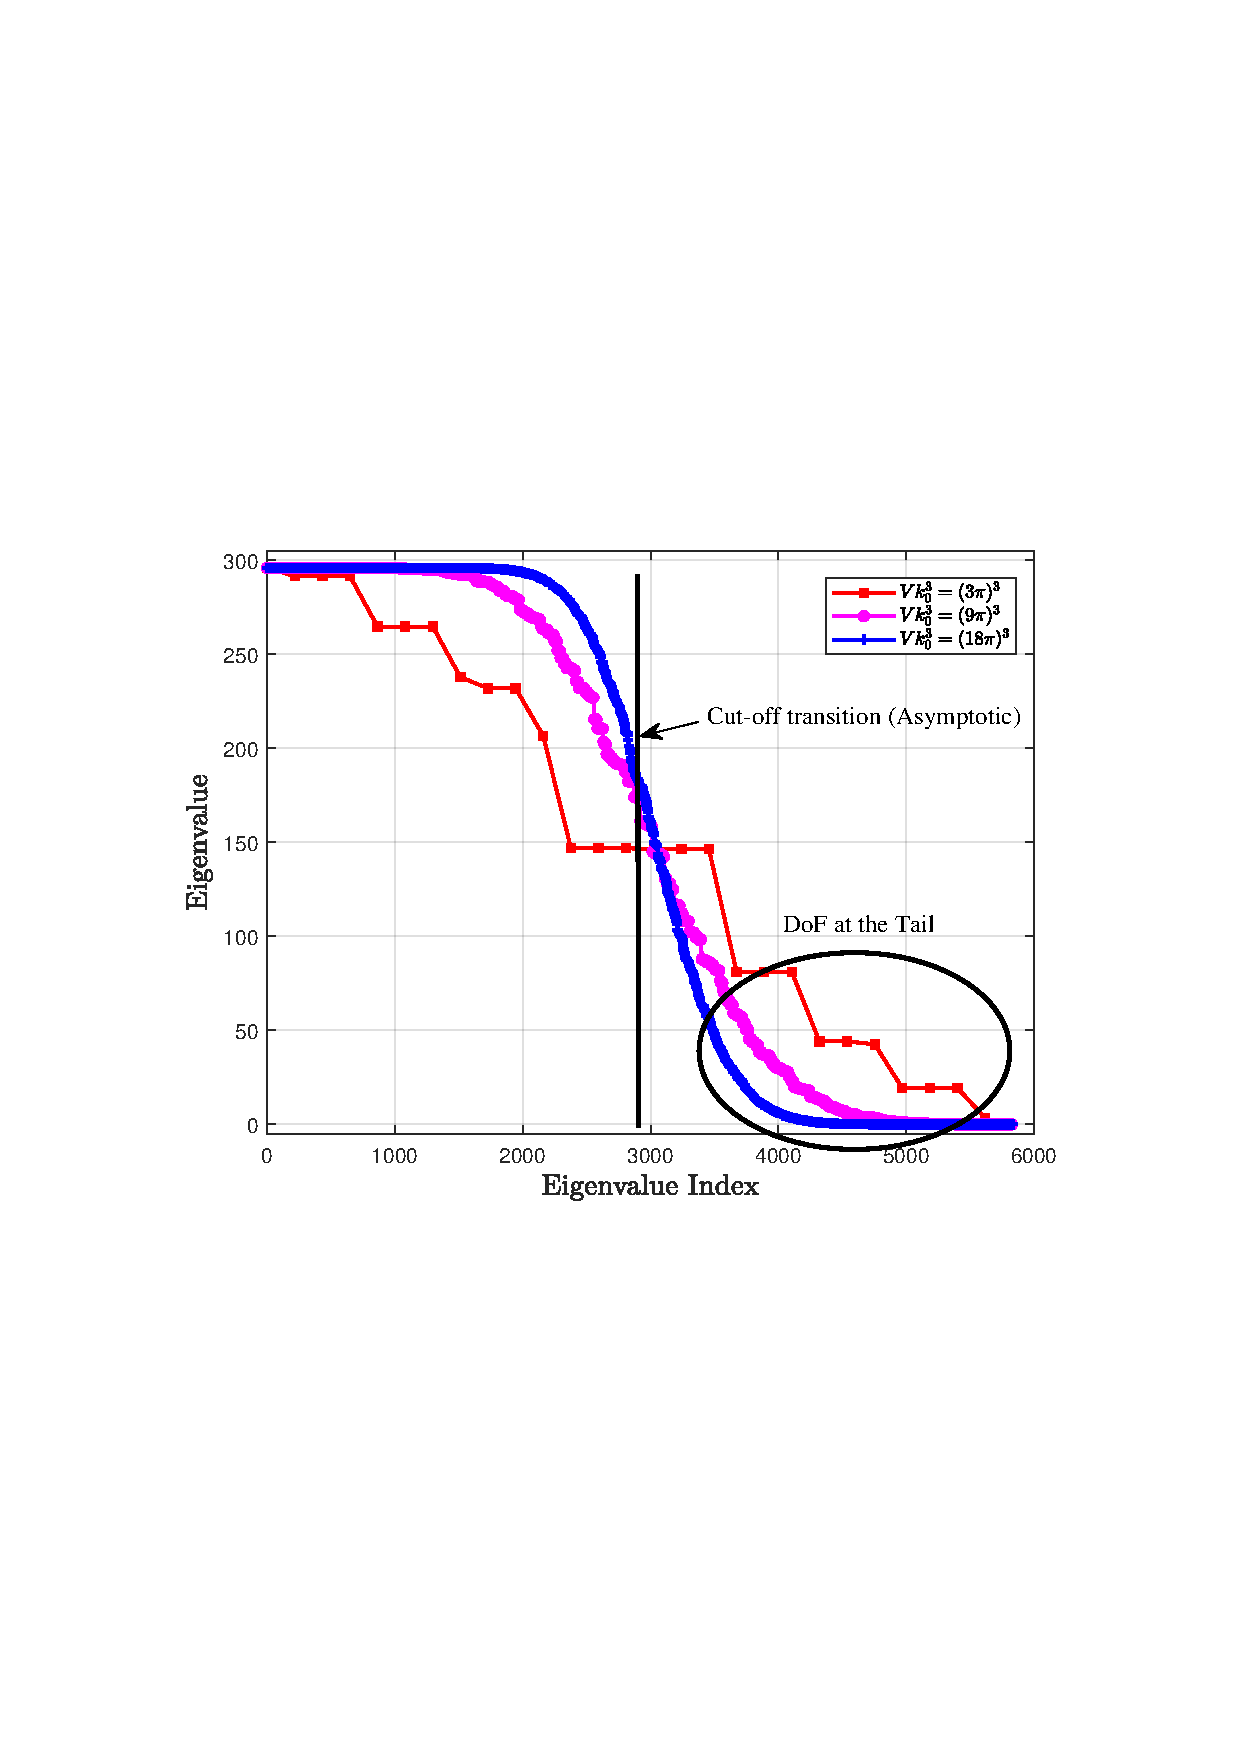
\includegraphics[width=0.7\textwidth]{figs/save_3d_different_Vk.pdf} 
		\caption{\color{red} The eigenvalues of three-dimensional Slepian concentration problem when $V k_0^3$ increases.} 
		\label{3d_Vk}
	\end{figure}



	\end{remark}
}
   
	In the above part we are analyzing the scenario where the direction of ${\bf k}$ is not restricted, which means that the incident wave to the receiver may have arbitrary direction, corresponding to general channel settings. Given a specific channel, the direction of the incident wave to the receiver may be constrained, which adds further restrictions on ${\bf k}$.  Specifically, new constraints ${\Omega}_1 \subset {\Omega}=\{\hat{\bf k}: \left\| \hat{\bf k} \right\|=1\}$ on $\hat{\bf k}$ can be introduced, which is determined by the concentration region of the electromagnetic field caused by the scattering channel. {\color{red} The restrictions on $k$ have been used in channel modeling schemes\cite{pizzo2022fourier}, as a tool to depict the wavenumber domain characteristics caused by the scatterers.
	It has also been used for DoF analysis\cite{poon2005degrees}, where asymptotic conclusions about the channel DoF are obtained based on one-dimensional Slepian concentration problem. } In this paper, we can have the following transform in three dimensional space
	\begin{equation}
		\begin{aligned}
			f({\bf x})=(2\pi)^{-3}\int_0^{k_0} \int_{{\Omega}_1 \subset {\Omega}=\{\hat{\bf k}: \left\| \hat{\bf k} \right\|=1\}} F({\bf k})e^{{\rm j}{\bf k}\cdot {\bf x}}{\rm d}^2S {\rm d}{k},
		\end{aligned}
		\label{eqn_wavenumber_constraint1}
	\end{equation}
	or
	\begin{equation}
		\begin{aligned}
			f({\bf x})=(2\pi)^{-3}\int_{k_1}^{k_0} \int_{{\Omega}_1 \subset {\Omega}=\{\hat{\bf k}: \left\| \hat{\bf k} \right\|=1\}} F({\bf k})e^{{\rm j}{\bf k}\cdot {\bf x}}{\rm d}^2S {\rm d}{k}.
		\end{aligned}
		\label{eqn_wavenumber_constraint2}
	\end{equation}
	In single-frequency scenario, it corresponds to
	\begin{equation}
		\begin{aligned}
			f({\bf x})=(2\pi)^{-3}\int_{{\Omega}_1 \subset {\Omega}=\{\hat{\bf k}: \left\| \hat{\bf k} \right\|=1\}}k_0^2F_1(\theta,\phi)e^{{\rm j}k_0\hat{\bf k}\cdot {\bf x}}{\rm d}^2S.
		\end{aligned}
		\label{eqn_wavenumber_constraint3}
	\end{equation}
	
	
Since ${\Omega}_1$ may have complicated shapes, which makes the aforementioned scheme that integrating from wavenumber domain hard to analyze, we need to find another way to solve the concentration problem. It is shown that the solving the integral equation of the concentration problem from either of the two domains that are Fourier and inverse Fourier transforms of each other yields consistent eigenvalues\cite{beylkin2007grids}. Therefore, if the concentration region in the space domain has regular shapes, we can obtain the kernel function by integrating from the spatial domain, which is easier. Assume that the spatial concentration region is a ball which satisfies $\left\| {\bf x} \right\|\leqslant r_0$, we can obtain the kernel function as
\begin{equation}
	\begin{aligned}
		D(\hat{\bf k},\hat{\bf k}') &= (2\pi)^{-3}\int_{\mathcal{K}} e^{{\rm j}k{\bf x}\cdot(\hat{\bf k}-\hat{\bf k}')}{\rm d}^3{\bf x}\Bigg|_{k=k_0} 
		\\&= \frac{1}{2\pi^2} \left( \frac{\sin r_0k_0\left\| \hat{\bf k}-\hat{\bf k}' \right\|}{k_0^3\left\| \hat{\bf k}-\hat{\bf k}' \right\|^3}-\frac{r_0\cos r_0k_0\left\| \hat{\bf k}-\hat{\bf k}' \right\|}{k_0^2\left\| \hat{\bf k}-\hat{\bf k}' \right\|^2} \right).
	\end{aligned}
\end{equation}
If the spatial concentration region is a cuboid, which satisfies $\left| x_x \right|\leqslant a_x$, $\left| x_y \right|\leqslant a_y$ and $\left| x_z \right|\leqslant a_z$, we can obtain the kernel function as
\begin{equation}
	\begin{aligned}
		D(\hat{\bf k},\hat{\bf k}') &= (2\pi)^{-3}\int_{-a_x}^{a_x}\int_{-a_y}^{a_y}\int_{-a_z}^{a_z} e^{{\rm j}k{\bf x}\cdot(\hat{\bf k}-\hat{\bf k}')}{\rm d}^3{\bf x}\Bigg|_{k=k_0}
		\\& = \frac{\sin(a_x(k_x-k_x'))}{\pi(k_x-k_x')}\frac{\sin(a_y(k_y-k_y'))}{\pi(k_y-k_y')}\frac{\sin(a_z(k_z-k_z'))}{\pi(k_z-k_z')}\Bigg|_{k=k_0}.
	\end{aligned}
\end{equation}
Then, corresponding to \eqref{eqn_wavenumber_constraint1}, the concentrated functions satisfy the following integral equation
\begin{equation}
	\lambda_i \phi_i({\bf k}) = \int_0^{k_0}\int_{{\Omega}_1 \subset {\Omega}=\{\hat{\bf k}': \left\| \hat{\bf k}' \right\|=1\}} D({\bf k},{\bf k}')\phi_i({\bf k}'){\rm d}^3{\bf k}'.
	\label{eqn_ball_wavenumber_constraint}
\end{equation}
Corresponding to \eqref{eqn_wavenumber_constraint2}, the concentrated functions satisfy the following integral equation
\begin{equation}
	\lambda_i \phi_i({\bf k}) = \int_{k_1}^{k_0}\int_{{\Omega}_1 \subset {\Omega}=\{\hat{\bf k}': \left\| \hat{\bf k}' \right\|=1\}} D({\bf k},{\bf k}')\phi_i({\bf k}'){\rm d}^3{\bf k}'.
\end{equation}
Corresponding to \eqref{eqn_wavenumber_constraint3}, the concentrated functions satisfy the following integral equation
\begin{equation}
	\lambda_i \phi_i(\hat{\bf k}) = \int_{{\Omega}_1 \subset {\Omega}=\{\hat{\bf k}': \left\| \hat{\bf k}' \right\|=1\}} D(\hat{\bf k},\hat{\bf k}')\phi_i(\hat{\bf k}'){\rm d}^2\hat{\bf k}'.
\end{equation}
%The DoF is then 
%\begin{equation}
%	\begin{aligned}
%		N^{3D} = \sum_{i=1}^\infty \lambda_i = \int_{\Omega_1}D(\hat{\bf k},\hat{\bf k}){\rm d}\hat{\bf k} = \frac{\mathcal{A}_{\Omega_1}a_xa_ya_z}{\pi^3}.
%	\end{aligned}
%\end{equation}
	
%	For two-dimensional antenna surface, if we only consider $x$ and $y$ axes and uses the two-dimensional Fourier transform, the Slepian's concentration problem follows (\ref{eq_2d_fourier}) to (\ref{eq_2d_dof}), which coincides the result in \cite{pizzo2022nyquist} using Landau's formula. However, this result is not accurate because an extra term should be added from the $z$ axis omitted in the two-dimensional Fourier transform. From the three-dimensional case, now we try to modify the derivation process. Since we have $\frac{\partial k_z}{\partial k_x} = \frac{-k_x}{\sqrt{k_0^2-k_x^2-k_y^2}}$ and $\frac{\partial k_z}{\partial k_y} = \frac{-k_y}{\sqrt{k_0^2-k_x^2-k_y^2}}$, we can obtain
%		\begin{equation}
%	\begin{aligned}
%		f({\bf x})&=(2\pi)^{-3}\int_{{\Omega}=\{\hat{\bf k}: \left\| \hat{\bf k} \right\|=k_0^2\}}F({k}_x,{k}_y,{k}_z)e^{{\rm j}{\bf k}\cdot {\bf x}}{\rm d}S
%		\\& = (2\pi)^{-3}\int_{k_x^2+k_y^2\leqslant k_0^2}\frac{k_0e^{{\rm j}\sqrt{k_0^2-k_x^2-k_y^2}x_z}F_2(k_x,k_y)}{\sqrt{k_0^2-k_x^2-k_y^2}}\\&~~~~e^{{\rm j}(k_xx_x+k_yx_y)}{\rm d}k_x{\rm d}k_y,
%	\end{aligned}
%\end{equation}
%and
%	\begin{equation}
%	\begin{aligned}
%		F({\bf k}) = \int_{-\infty}^{+\infty}f({\bf x})e^{-{\rm j}{\bf k}\cdot {\bf x}}{\rm d}{\bf x},
%	\end{aligned}
%\end{equation}
%	

	\subsection{Slepian concentration problem in four-dimensional space-time domain}
	\label{subsec_4d_slepian}
	
	After discussing the theoretical analysis in the three-dimensional domain, we now go further into the four-dimensional space-time domain, which fully characterizes the electromagnetic fields. Moreover, only with the change in the time domain can we transmit information in practical wireless communication systems.
	
	For ease of analysis, we introduce the following theorem from \cite{ihara1993information}.
	
	\begin{theorem}
		\cite{ihara1993information} Let $\mathcal{H}$ be a Hilbert space. Let $\mathcal{H}_1$ and $\mathcal{H}_2$ be two subspaces of $\mathcal{H}$. We have $\Pi_1$ and $\Pi_2$ be two projection operators that satisfy $\Pi_1 x \in \mathcal{H}_1$ and $\Pi_2 x \in \mathcal{H}_2$ for $x \in \mathcal{H}$. Let $A = \Pi_1 \Pi_2 \Pi_1$ and $B = \Pi_2 \Pi_1 \Pi_2$. Then, there exist complete orthonormal bases $\{\phi_n \}_{n=1}^{\infty}$ for $\mathcal{H}_1$ and $\{\psi_n \}_{n=1}^{\infty}$ for $\mathcal{H}_2$ that span the eigenspaces of $A$ and $B$ separately. The eigenvalues of $A$ and $B$ form the same sequence $\{\lambda_n \}_{n=1}^{+\infty}$, which satisfies
		\begin{subequations}
			\begin{align} 
				&A\phi_n = \lambda_n \phi_n, \label{Aphi}\\
				& B \psi_n = \lambda_n \psi_n,  \label{Bpsi}\\
				& \langle \phi_m \ket{\psi_n} = \sqrt{\lambda_n} \delta_{mn},
			\end{align}
		\end{subequations}
		for arbitrary $m,n\in \mathbb{Z}^+$.
	\end{theorem}
	\begin{remark}
		From the projection operators we can obtain the same mathematical forms as (\ref{eigenfunction_3d}), leading to the same eigenfunctions and eigenvalues. 
	\end{remark}
	Now we use {\bf Theorem 1} to analyze the DoF of the received electromagnetic fields in the four-dimensional space-time domain. In our considered scenario, the Hilbert space $\mathcal{H}_1$ contains the electromagnetic fields that are constrained in space domain $\mathcal{R}$ and constrained in time domain $\mathcal{T}$. The Hilbert space $\mathcal{H}_2$ contains the electromagnetic fields that are constrained in frequency domain $\mathcal{W}$ and constrained in wavenumber domain $\mathcal{K}$. Moreover, $\mathcal{H}_2$ also satisfies $w^2 = c^2\left\| {\bf k} \right\|^2 $ according to electromagnetic constraints. Therefore, we have $\Pi_1f = \mathcal{B}_1 f $ and $\Pi_2 f = \mathcal{F}^{-1} \mathcal{B}_2 \mathcal{F} f$, where 
	\begin{equation}
		\begin{aligned}
			\mathcal{B}_1 f = \left\{\begin{matrix}
			f	&  t\in \mathcal{T} \& {\bf x} \in \mathcal{R},  \\
			0	&  {\rm otherwise},
			\end{matrix}\right.
		\end{aligned}
	\end{equation}
	and
		\begin{equation}
		\begin{aligned}
			\mathcal{B}_2 f = \left\{\begin{matrix}
				f	&  w= \pm c \left\| {\bf k} \right\| \& {\bf k} \in \mathcal{K},  \\
				0	&  {\rm otherwise}.
			\end{matrix}\right.
		\end{aligned}
	\end{equation}
	The concentration regions $\mathcal{H}_1$ and $\mathcal{H}_2$ constructed from the electromagnetic constraints are shown in Fig. \ref{H1H2projection}.
	
	Noted that we can abbreviate $B$ as $\Pi_2 \Pi_1$ since the eigenfunctions $\psi_n$ are in $\mathcal{H}_2$. We have 
	\begin{equation}
		\begin{aligned}
		(\Pi_2 \Pi_1 f)({\bf x}',t') &=  (\mathcal{F}^{-1} \mathcal{B}_2 \mathcal{F} \mathcal{B}_1f)({\bf x},t)
		\\& = \int_{w= \pm c \left\| {\bf k} \right\| \& {\bf k} \in \mathcal{K}} e^{{\rm j}{\bf k}\cdot{\bf x}-{\rm j}wt} \int_{t\in \mathcal{T} \& {\bf x} \in \mathcal{R}} e^{-{\rm j}{\bf k}\cdot {\bf x}'+{\rm j}wt' } f({\bf x}',t'){\rm d}^3{\bf x}'{\rm d}t' {\rm d}^3{\bf k}{\rm d}w
		\\& = \int_{t\in \mathcal{T} \& {\bf x} \in \mathcal{R}}  \int_{w= \pm c \left\| {\bf k} \right\| \& {\bf k} \in \mathcal{K}} e^{{\rm j}{\bf k}\cdot({\bf x}-{\bf x}')-{\rm j}w(t-t')}
		 {\rm d}^3{\bf k}{\rm d}w f({\bf x}',t'){\rm d}^3{\bf x}'{\rm d}t',
		\end{aligned}
	\end{equation}
	and the integral equation is $(\Pi_2 \Pi_1 f)({\bf x}',t') = \lambda f({\bf x},t)$.
	
		
	\begin{figure}
		\centering 
		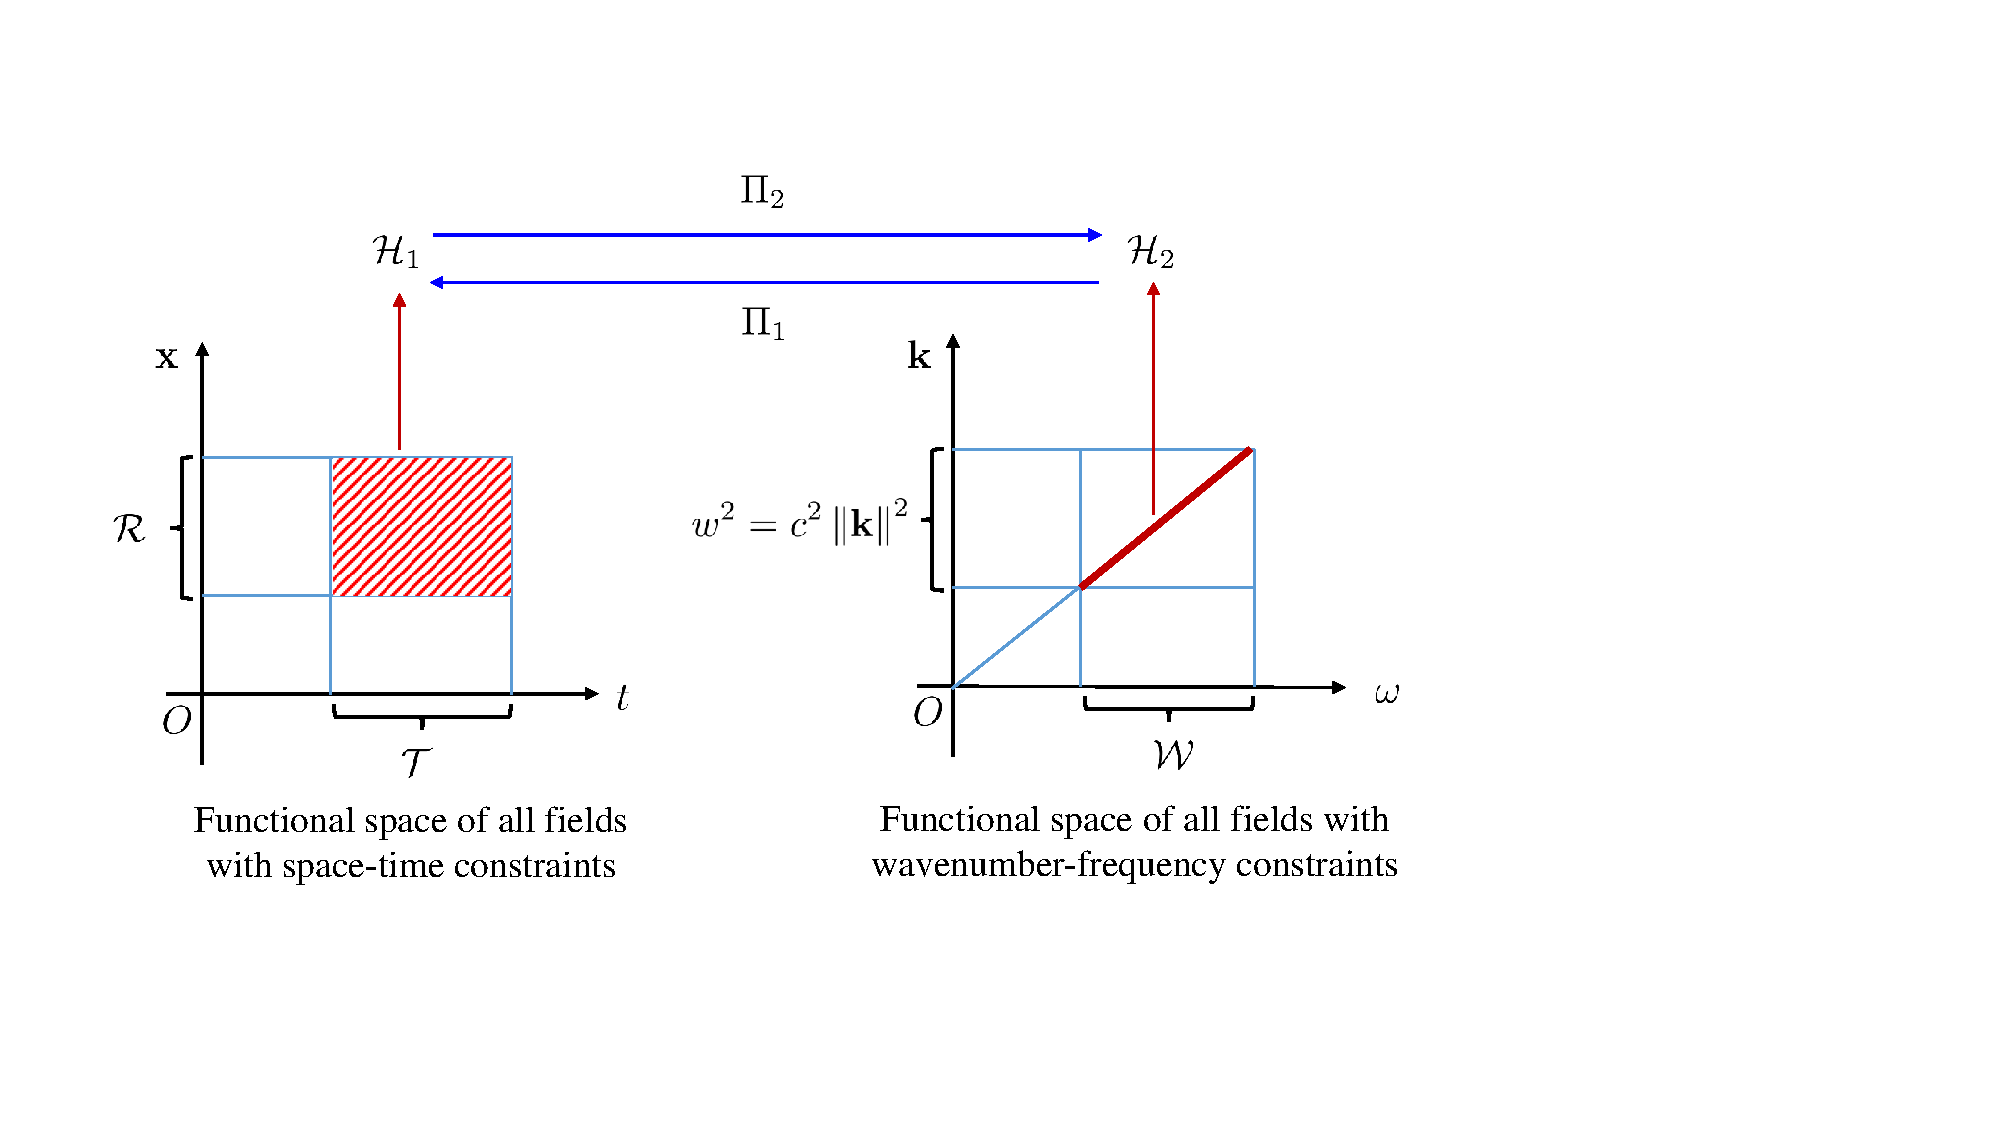
\includegraphics[width=0.7\textwidth]{figs/H1H2projection.pdf} 
		\caption{The two functional spaces $\mathcal{H}_1$ and $\mathcal{H}_2$ include all fields with space-time constraints and all fields with wavenumber-frequency constraints separately. $\mathcal{H}_1$ and $\mathcal{H}_2$ are subspaces of $\mathcal{H}$. Through projection operators $\Pi_1$ and $\Pi_2$ we can project arbitrary $x \in \mathcal{H}$ onto $\mathcal{H}_1$ and $\mathcal{H}_2$.  } 
		\label{H1H2projection}
	\end{figure}
	
	
	If we only consider a single time point, we set $t=t'=t_0$, the eigenfunction can be simplified as 
	\begin{equation}
		\begin{aligned}
			\int_{{\bf x} \in \mathcal{R}}  \int_{ {\bf k} \in \mathcal{K}} e^{{\rm j}{\bf k}\cdot({\bf x}-{\bf x}')}
			{\rm d}^3{\bf k} f({\bf x}',t_0){\rm d}^3{\bf x}' = \lambda f({\bf x},t_0).
		\end{aligned}
	\end{equation}
	It is worth noting that by omitting time interval, the eigenfunction degenerates to the form in {\bf Section \ref{subsec_3d_slepian}}, which verifies the above analysis in three-dimensional space. 
	
	Now we consider using a continuous time interval. Moreover, we assume that the frequency band is $\omega \in [-ck_0, ck_0]$ and the wavenumber domain satisfies $\left\| {\bf k} \right\| \leqslant k_0$. Then we have 
	\begin{equation}
		\begin{aligned}
			\int_{w= \pm c \left\| {\bf k} \right\| \& {\bf k} \in \mathcal{K}} e^{{\rm j}{\bf k}\cdot({\bf x}-{\bf x}')-{\rm j}w(t-t')}
			{\rm d}^3{\bf k}{\rm d}w
			= & \int_{0}^{k_0} \int_{{\Omega}=\{\hat{\bf k}: \left\| \hat{\bf k} \right\|=1\}} e^{{\rm j}k \hat{\bf k}\cdot({\bf x}-{\bf x}')} {\rm d}^2S 2\cos(ck(t-t')) k^2{\rm d}k
			\\ = & \int_{0}^{k_0} 4\pi \frac{\sin k \left\| {\bf x}-{\bf x}' \right\|}{k \left\| {\bf x}-{\bf x}' \right\|}  2\cos(ck(t-t'))k^2{\rm d}k,
		\end{aligned}
	\end{equation}
	which can be further simplified to (\ref{equ_kernel_expression}).
	By substituting the kernel function in $\Pi_2 \Pi_1 f({\bf x}',t') = \lambda f({\bf x},t)$, we can obtain the eigenvalues and eigenfunctions which correspond to DoF and orthogonal patterns for the electromagnetic fields.
	
			\begin{figure*}
		\begin{equation}
			\begin{aligned}
				%				&\frac{2\pi e^{-{\rm j}ck_0(t-t')}}{\left\| {\bf x}-{\bf x}' \right\|(\left\| {\bf x}-{\bf x}' \right\|^2-c^2(t-t')^2)^2} \Bigg(2{\rm j}c \left\| {\bf x}-{\bf x}' \right\|(t-t') e^{{\rm j}ck_0(t-t')}
				%				+ \left\| {\bf x}-{\bf x}' \right\| \Big( -k_0\left\| {\bf x}-{\bf x}' \right\|^2 + c(t-t')(-2{\rm j}+c(t-t')k_0)  \Big)
				%				\\&\cos(k_0 \left\| {\bf x}-{\bf x}' \right\|) + \Big( \left\| {\bf x}-{\bf x}' \right\|^2 (1-{\rm j}ck_0(t-t')) + c^2(t-t')^2(1+{\rm j}ck_0(t-t')) \Big) \sin(k_0 \left\| {\bf x}-{\bf x}' \right\|)\Bigg)
				-\frac{4\pi\Big(- \left\| {\bf x}-{\bf x}' \right\| + \left\| {\bf x}-{\bf x}' \right\| \cos(k_0\left\| {\bf x}-{\bf x}' \right\|)\cos(ck_0(t-t')) + c(t-t')\sin(k_0\left\| {\bf x}-{\bf x}' \right\|)\sin(ck_0(t-t'))  \Big)}{\left\| {\bf x}-{\bf x}' \right\|(\left\| {\bf x}-{\bf x}' \right\|^2-c^2(t-t')^2)^2}
			\end{aligned}
			\label{equ_kernel_expression}
		\end{equation}
		{\noindent} \rule[-10pt]{18cm}{0.05em}
	\end{figure*}

	{\color{red}
	\begin{remark}
		(relationship and differences between cases with different dimensions) After introducing and analyzing all the concentration problems based on one-dimensional, two-dimensional, three-dimensional and four-dimensional cases, now we will discuss the relationship and differences between them. First of all, the one-dimensional case, although originally used in the time-frequency domain, can be used in the space-wavenumber domain considering only one dimension. In other words, this case corresponds to the model with ideal transceivers on a line in the spatial domain. In the wavenumber domain, two of the three variables $k_x$, $k_y$, and $k_z$ are omitted. The constraint region in this case is the projection of the original constraint region in the three-dimensional domain to only one dimension of it. The two-dimensional case is similar, which is not repeated here. It is easy to observe that some structural information is lost in such a projection. For example, we show the three different structures of constraint regions in the wavenumber domain that have been discussed in Section \ref{subsec_3d_slepian} in previous subsections. These three structures will lead to different DoFs and sampling schemes in the spatial domain. However, when projecting them to the two-dimensional domain as formulated in (\ref{eqn_2d_integral}), all of them degenerate to the same disc, losing the information that exists in the third dimension. Therefore, we claim that analyzing the concentration problem in the three-dimensional space-wavenumber domain is better than lower dimensions, which preserves more information of the original electromagnetic field. 

		Besides the three-dimensional space-time domain, we further consider the time domain to extend the dimensions of the problem to four. By incorporating the time domain into the system model, it becomes possible to characterize the joint properties of electromagnetic waves across both space and time domains in a more unified manner. This enables the construction of time–space joint electromagnetic bases, which, in contrast to conventional designs that decouple space and time, may bring additional performance gains. The underlying reason lies in the dispersion relation from Maxwell's equations, which intrinsically couples the Fourier representation in the time domain with that in the space domain, thereby making the two domains inseparable in essence. It is interesting to find that the Minkowski spacetime interval $s^2 = c^2(t-t')^2 - \left\| {\bf x}-{\bf x}' \right\|^2$ exists in the four-dimensional integral kernel function (\ref{equ_kernel_expression}), which reflects the inherent compatibility of Maxwell’s equations with the framework of special relativity \cite{schwinger2019classical}. Since it is the pole of the kernel function, it is associated with the eigenmodes of the electromagnetic field. When this term equals 0, we can get the light-cone relation $\left\| {\bf x}-{\bf x}' \right\|= c|t-t'|$, which reflects the causal structure of the field when transmitting.


			\begin{figure}
		\centering 
		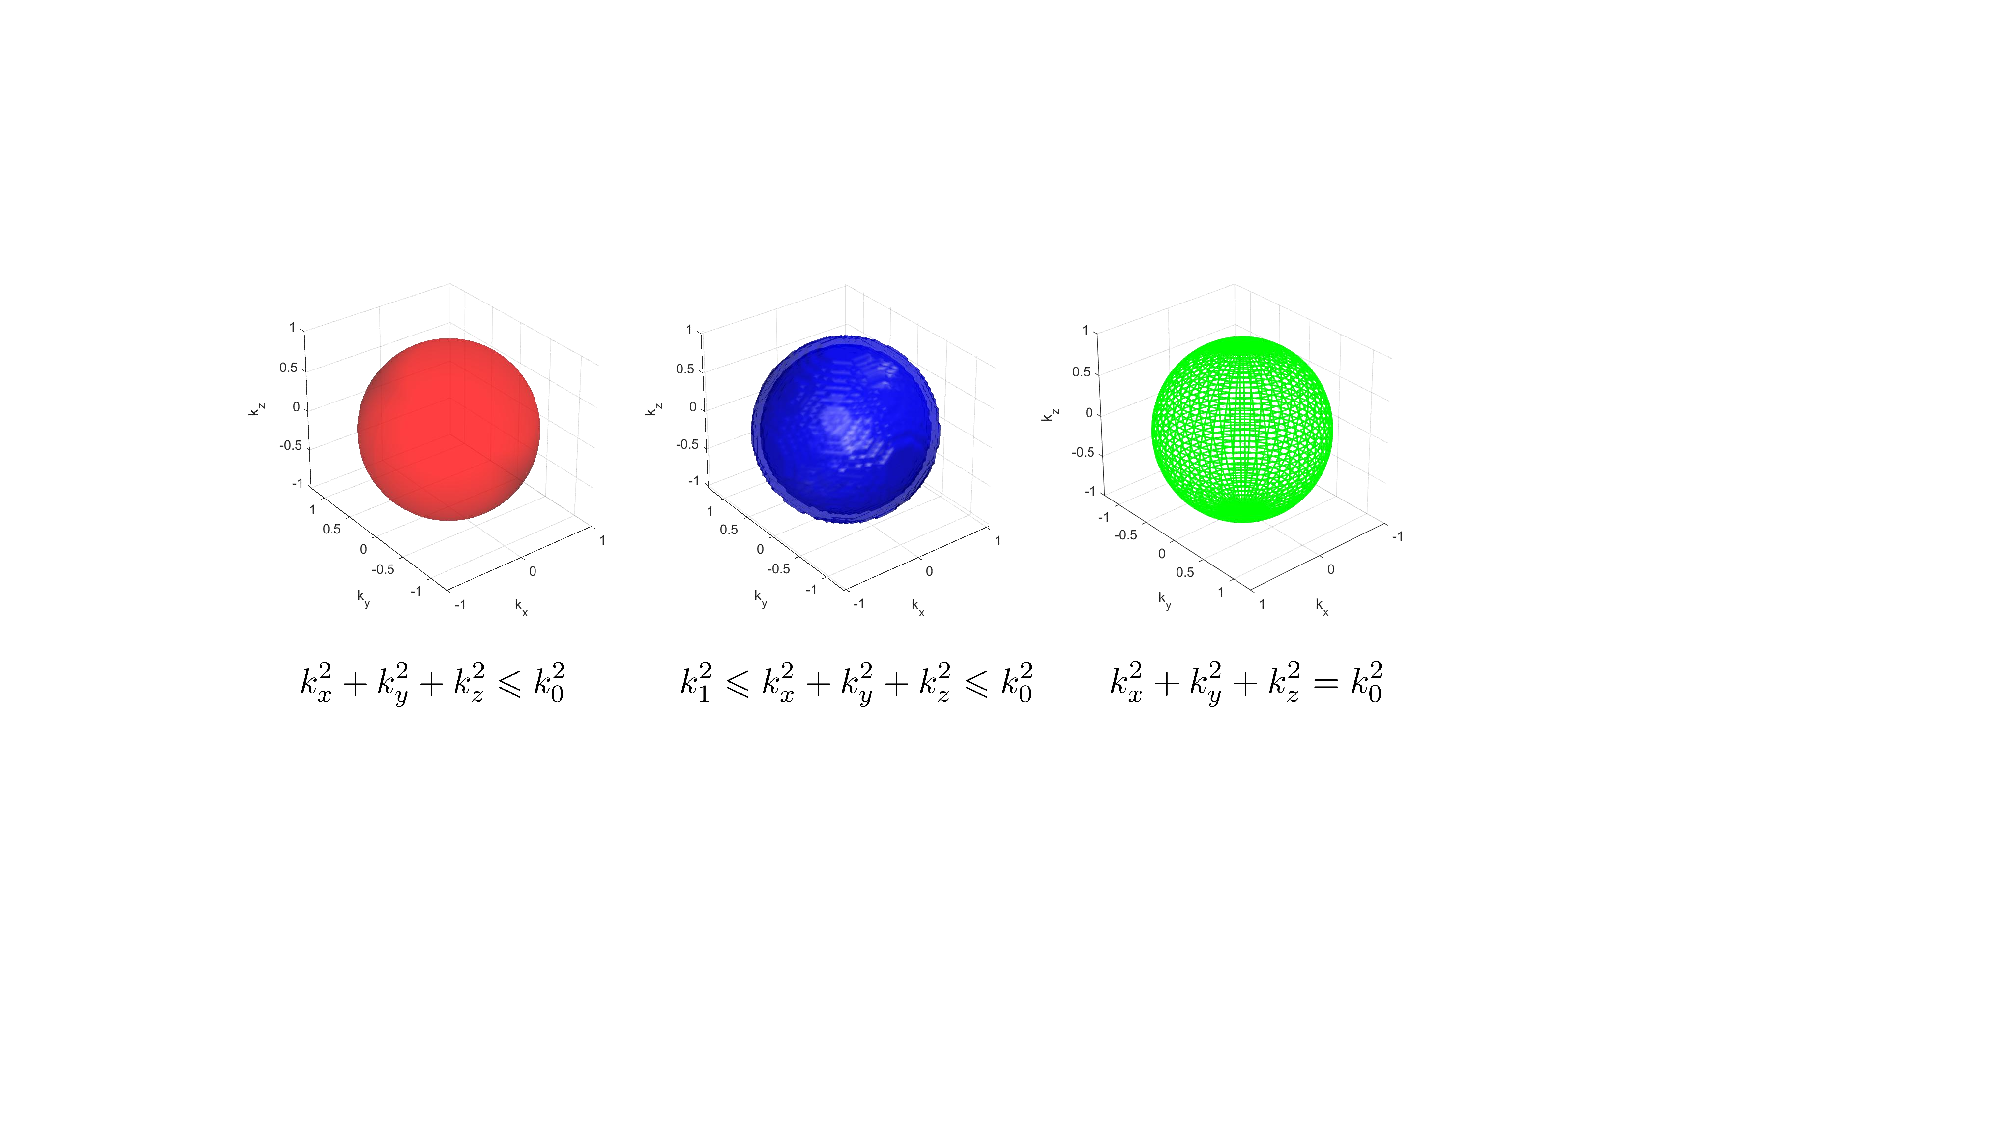
\includegraphics[width=0.7\textwidth]{figs/Three_d_comparison.pdf} 
		\caption{\color{red} Three different structures of constraint regions in wavenumber domain.} 
		\label{Three_d_comparison}
	\end{figure}
	\end{remark}
	}
	

	{\color{red}
	\begin{remark}
		(motivation and novelty of studying the DoF)
		After the theoretic analysis of the DoF, we can now present the motivation and novelty of studying the DoF in the paper from the following two perspectives: 1) The degrees of freedom (DoF) of an electromagnetic field characterize the dimension of the functional space it spans, i.e., the minimum number of orthogonal base functions required for its representation. Therefore, the DoF analyzing framework can offer a more fundamental and physically intuitive criterion for determining the number of antennas required in array design to approach optimal system performance compared to mutual information or capacity analysis. 2) While capacity and mutual information analysis in existing works rely on a specific channel model, in this paper the fDoF analysis is an upperbound covering all kinds of channel conditions, which only relies on the characteristics of the transceivers and is different from the results obtained from capacity or mutual information analysis. We have also discussed the relationship between fDoF and cDoF, which relies on a specific channel. Therefore, our analysis of DoF has provided some new insights compared to existing capacity or mutual information analysis. 
	\end{remark}
	}
	
	\section{Numerical simulation}
	
	After showing that the DoF analyzed in this paper provides performance upperbound for wireless communication systems, in this part we will provide numerical simulations of the eigenvalues and eigenfunctions based on the theoretical derivations. 

	{\color{red}
	It is worth noting that all the theoretical derivations above are based on the electromagnetic fields constrained in continuous regions. The distribution of eigenvalues characterizes the number of eigenfunctions required to approximate any desired continuous electromagnetic field using the obtained eigenfunction basis, which requires solving the eigen-problem of an integral operator $T := \phi({\bf x}) \rightarrow \int_{\mathcal{R}} K({\bf x},{\bf x}')\phi({\bf x}') {\rm d}^3 {\bf x}'$ or $T := \phi({\bf x},t) \rightarrow \int_{\mathcal{T}}\int_{\mathcal{R}} K({\bf x},t,{\bf x}',t')\phi({\bf x}',t') {\rm d}^3 {\bf x}'{\rm d} {t}'$ with kernel function $K$ solved in {\bf Section} \ref{subsec_3d_slepian} and \ref{subsec_4d_slepian}. Take the four-dimensional case as an example, the eigen-problem is formulated as the following integral equation
	\begin{equation}
		\lambda_i \phi_i({\bf x},t) = T \phi_i({\bf x},t).
	\end{equation}
	In the simulation part, we consider numerical discretization methods, which can be viewed as using a model that divides the continuous region into several spatially discretized regions. The discretization order $n$ corresponds to the number of antennas and time-observation points used in practical engineering problems, where each antenna provides one observation of the electromagnetic field within a given discretized spatial region. The eigenvalues and eigenvectors of the discretized matrix are then used as counterparts to the eigenvalues and eigenfunctions of the continuous operator in the theoretical analysis. To be more specific, we have a discretized matrix ${\bf K}$ with ${\bf K}_{i,j} = w_j K({\bf x}_i,t_i,{\bf x}_j,t_j)$, where ${w}_{i=1}^n$, ${\bf x}_{i=1}^n$, and $t_{i=1}^n$ are chosen by numerical integral quadrature rules on the regions $\mathcal{R}$ and $\mathcal{T}$. Then, the eigenproblem is formulated as the integral equation
	\begin{equation}
		\lambda'_i {\bf v} = {\bf K} {\bf v}.
	\end{equation}
	As the discretization order increases, Nyström’s method ensures that the matrix eigenvalues converge to those of the continuous operator, which can be found in {\bf Theorem 7} in \cite{spence1975convergence}. 
	}
	
	{\color{red} After discussing the rationality of the numerical schemes, we will now} simulate the eigenvalues of the Slepian concentration problem for three-dimensional antenna array based on (\ref{eigenfunction_3d}), where the kernel functions are provided in (\ref{equ_ball}), (\ref{equ_spherical_shell}), and (\ref{equ_sphere_surface}). The simulation results show the DoF upperbound when antennas are constrained in three-dimensional space.
	We show the DoF with different frequency bandwidths in Fig. \ref{different_frequency_setting}. The three-dimensional antenna array is $0.5\,{\rm m} \times 0.5\,{\rm m} \times 0.5\,{\rm m}$, sampled with $\lambda/2$ antenna spacing. The shape of the concentration region in the wavenumber domain is set to ball, spherical shell, and sphere surface, which correspond to different frequency settings.
	The maximum frequency is $3\,{\rm GHz}$. The ball corresponds to frequency band $[0,3]\,{\rm GHz}$. The thick shell has $2\,{\rm GHz}$ bandwidth. The thin shell has $150\,{\rm MHz}$ bandwidth. The sphere surface in the wavenumber domain corresponds to a single-frequency point at $3\,{\rm GHz}$. The figure shows that not all eigenvalues tend to a maximum or 0 for the broad-band scenario. On the contrary, a large transition band still exists, which means that the asymptotic conclusions of DoF are not accurate enough. For the narrow-band or single-frequency scenario, the eigenvalues decay very fast from the maximum value, which implies that asymptotic conclusions of DoF do not work.
	It can also be observed that when the frequency bandwidth tends to 0 (the thickness of the spherical shell in the wavenumber domain tends to 0), the eigenvalues converge to those in the case with the single-frequency point, which leads to non-zero DoFs and verifies the theoretical analysis. It also shows that the DoF is not linear with bandwidth in the narrow-band scenario.
	 
	
	\begin{figure}
		\centering 
		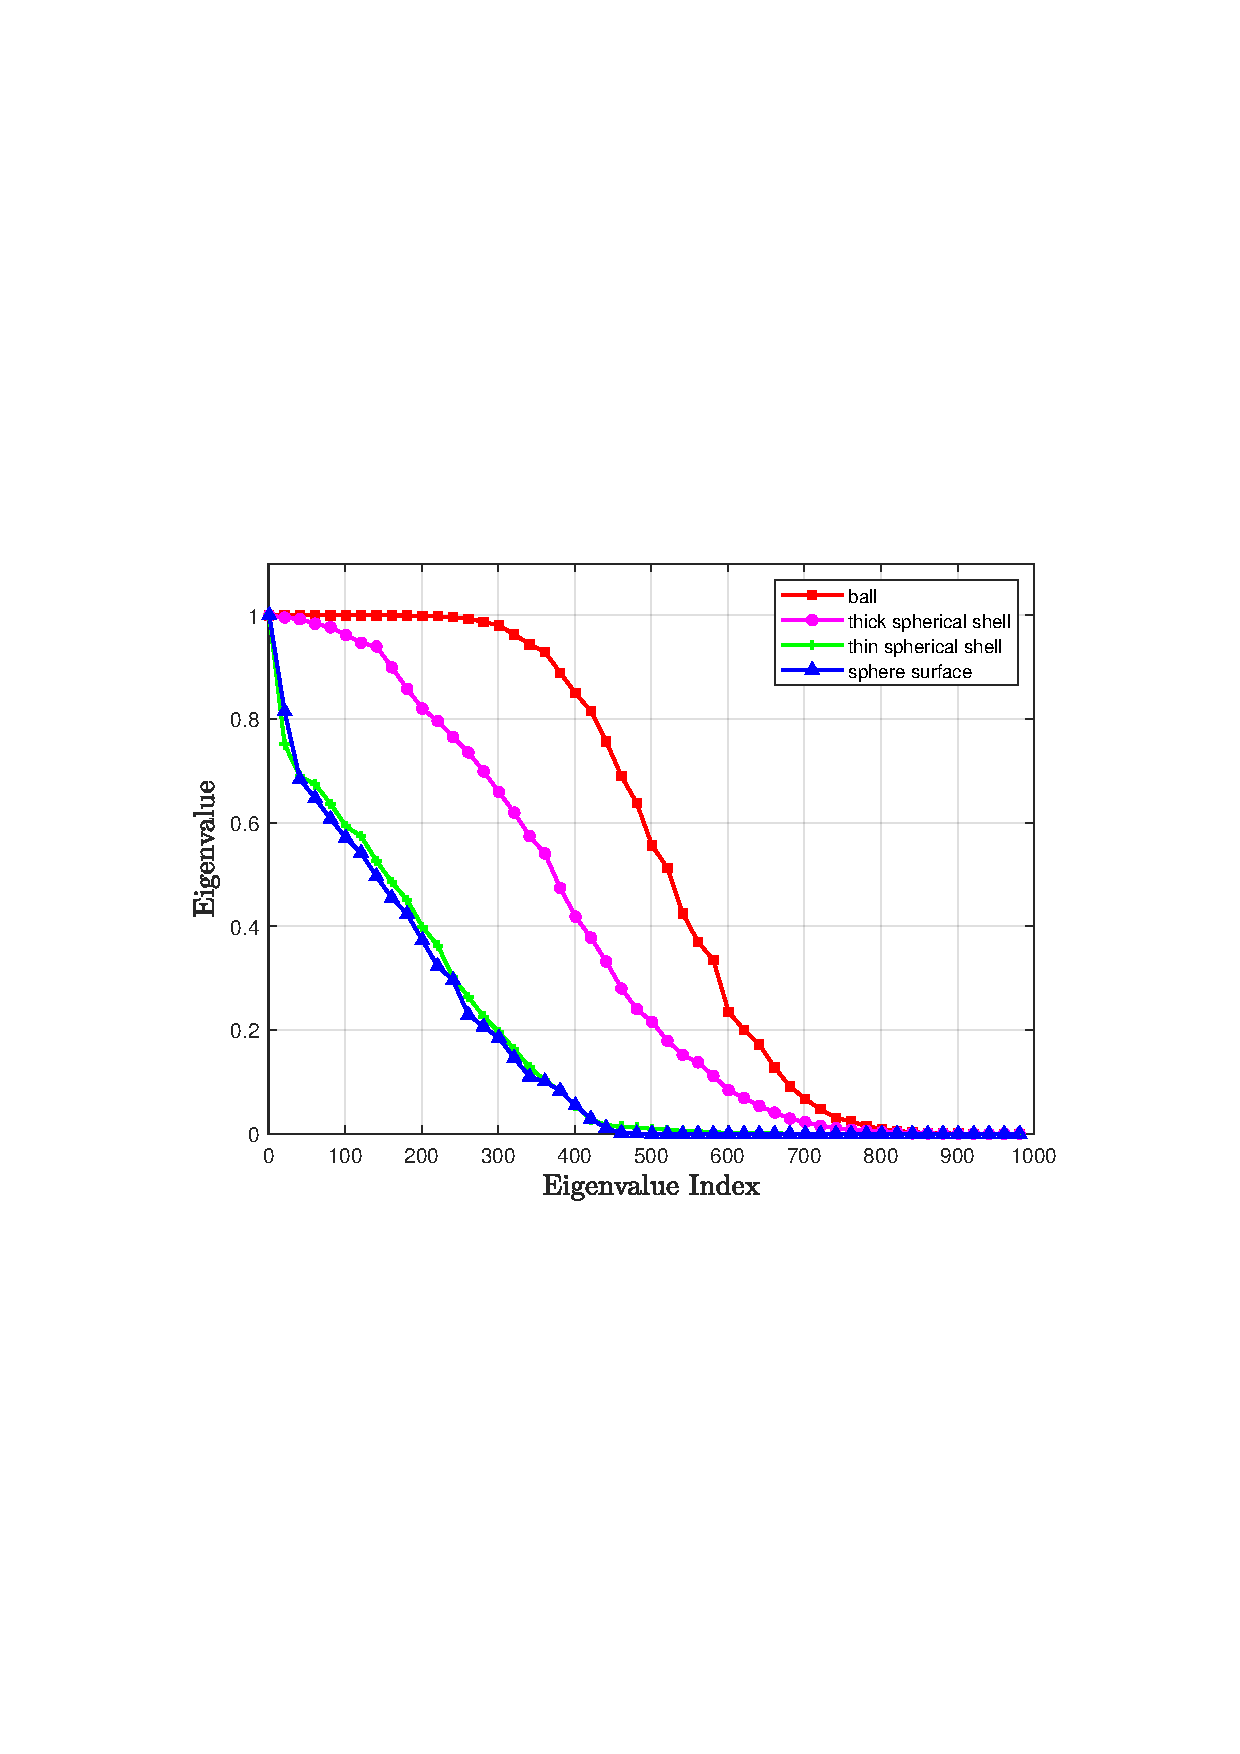
\includegraphics[width=0.7\textwidth]{figs/different_frequency_setting.pdf} 
		\caption{The DoF gain with different frequency band. The three-dimensional antenna array is $0.5\,{\rm m} \times 0.5\,{\rm m} \times 0.5\,{\rm m}$, sampled with $\lambda/2$ antenna spacing. The maximum frequency is $3\,{\rm GHz}$. The thick shell has $2\,{\rm GHz}$ bandwidth. The thin shell has $150\,{\rm MHz}$ bandwidth. The sphere surface in the wavenumber domain corresponds to single-frequency point at $3\,{\rm GHz}$.} 
		\label{different_frequency_setting}
	\end{figure}
	
	
	Then, we simulate the DoF gain with different heights in Fig. \ref{different_z_setting}. The three-dimensional antenna array is $0.5\,{\rm m} \times 0.5\,{\rm m} \times 0.05x\,{\rm m}$, sampled with $\lambda/2$ antenna spacing. $x$ is chosen to be $1$, $3$, $7$, and $10$ to represent three-dimensional antenna array with different heights (number of layers). It can be observed from Fig. \ref{different_z_setting} that extra space dimension brings DoF gain for the  electromagnetic fields, which means that by using three-dimensional antenna arrays, more DoFs may be obtained compared to traditional two-dimensional surface. 
	
	\begin{remark}
		The performance gain of three-dimensional antenna array may come from the enhancement of wave number domain resolution capability compared to two-dimensional antenna array. For the three-dimensional concentration problem with wavenumber domain constraint $k_x^2+k_y^2+k_z^2 \leqslant k_0^2$, it is easy to observe that it has the same asymptotic DoFs with the problem which has wavenumber domain constraint $k_x^2+k_y^2 \leqslant k_0^2$ and $|k_z| \leqslant \frac{2}{3}k_0$. The latter problem, which has a cylinder-shaped wavenumber domain constraint, can use separation of variables. To be clearer, it can be decomposed as a two-dimensional concentration problem with variables $k_x$ and $k_y$, which has eigenfunctions $\{\phi_i(k_x,k_y)\}_{i=1}^{+\infty}$, and a one-dimensional concentration problem with variables $k_z$, which has eigenfunctions $\{\phi_i(k_z)\}_{i=1}^{+\infty}$. Then we can observe that the eigenfunctions of the three-dimensional concentration problem, expressed as $\{\phi_i(k_x,k_y)\phi_j(k_z)\}_{i=1,j=1}^{+\infty}$, from a many-to-one mapping with the eigenfunctions of the two-dimensional concentration problem. In another word, it means that several waveforms in three-dimensional case project to the same waveform in two-dimensional case, showing the enhancement of wave number domain resolution capability by using three-dimensional array.
	\end{remark}
	
	\begin{figure}
		\centering 
		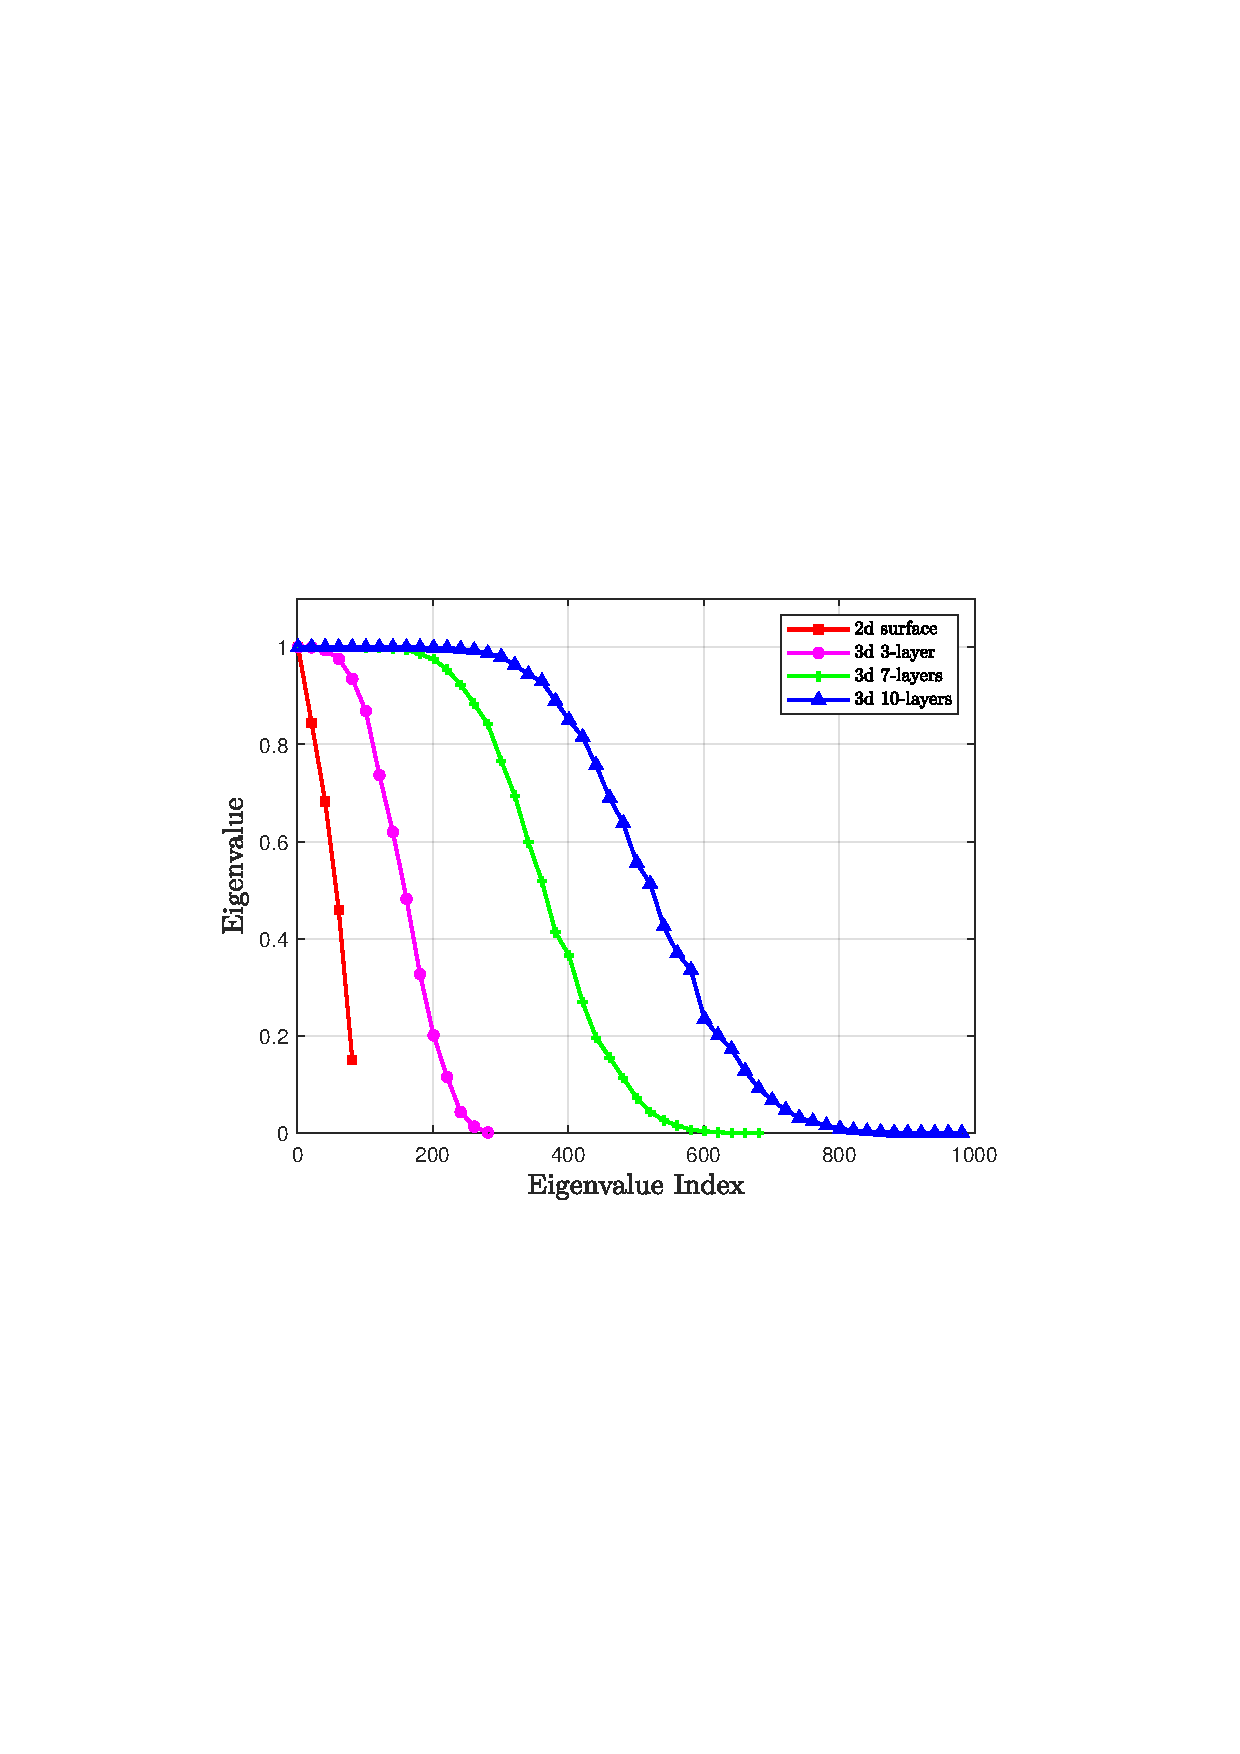
\includegraphics[width=0.7\textwidth]{figs/different_z_setting.pdf} 
		\caption{The DoF gain with different heights. The three-dimensional antenna array is $0.5\,{\rm m} \times 0.5\,{\rm m} \times 0.05x\,{\rm m}$, sampled with $\lambda/2$ antenna spacing. $x$ is chosen to be $1$, $3$, $7$ and $10$ to represent three-dimensional antenna array with different heights (number of layers).} 
		\label{different_z_setting}
	\end{figure}
		
		
	Next we discuss the near-optimal sampling scheme of antenna array. Noted that for the two-dimensional antenna array that simply omit the third spatial dimension, \cite{pizzo2022nyquist} shows that the half-wavelength sampling is the optimal scheme. On the one hand, this conclusion is approximate rather than completely accurate even for an ideal two-dimensional array. On the other hand, electromagnetic fields actually exist in three-dimensional space, which implies that simply ignoring one dimension may lead to model mismatch. In the following part we will show the spatial sampling scheme of ideal two-dimensional planar array based on the two-dimensional Slepian concentration problem. Then we will provide simulations based on three-dimensional models to provide more accurate and general conclusions on DoF.
		
		Fig. \ref{different_z_setting_2d} shows the eigenvalues of a two-dimensional Slepian concentration problem, which can be viewed as omitting the third dimension in space and wavenumber domain of electromagnetic field. The space concentration region is a rectangle, the size of which is $6\lambda \times 6\lambda$, with different antenna spacing in the simulation. The maximum frequency is $3\,{\rm GHz}$. It is worth noting that whatever the frequency bandwidth is, the concentration region in the space domain keeps the same, because the two-dimensional projections of solid sphere, spherical shell and sphere surface are all solid circles. 
		 It can be observed from Fig. \ref{different_z_setting_2d} that by applying half-wavelength sampling on the two-dimensional array, nearly all eigenvalues are above zero, which means that half-wavelength sampling is necessary to utilize the DoF of the electromagnetic fields. The number of non-zero eigenvalues of $\lambda/4$ sampling is a little larger than half-wavelength sampling, which introduces extra DoFs. Whether these DoFs are worth using relies on the error threshold in {\bf Definition 1}.
		 
		 \begin{figure}
		 	\centering 
		 	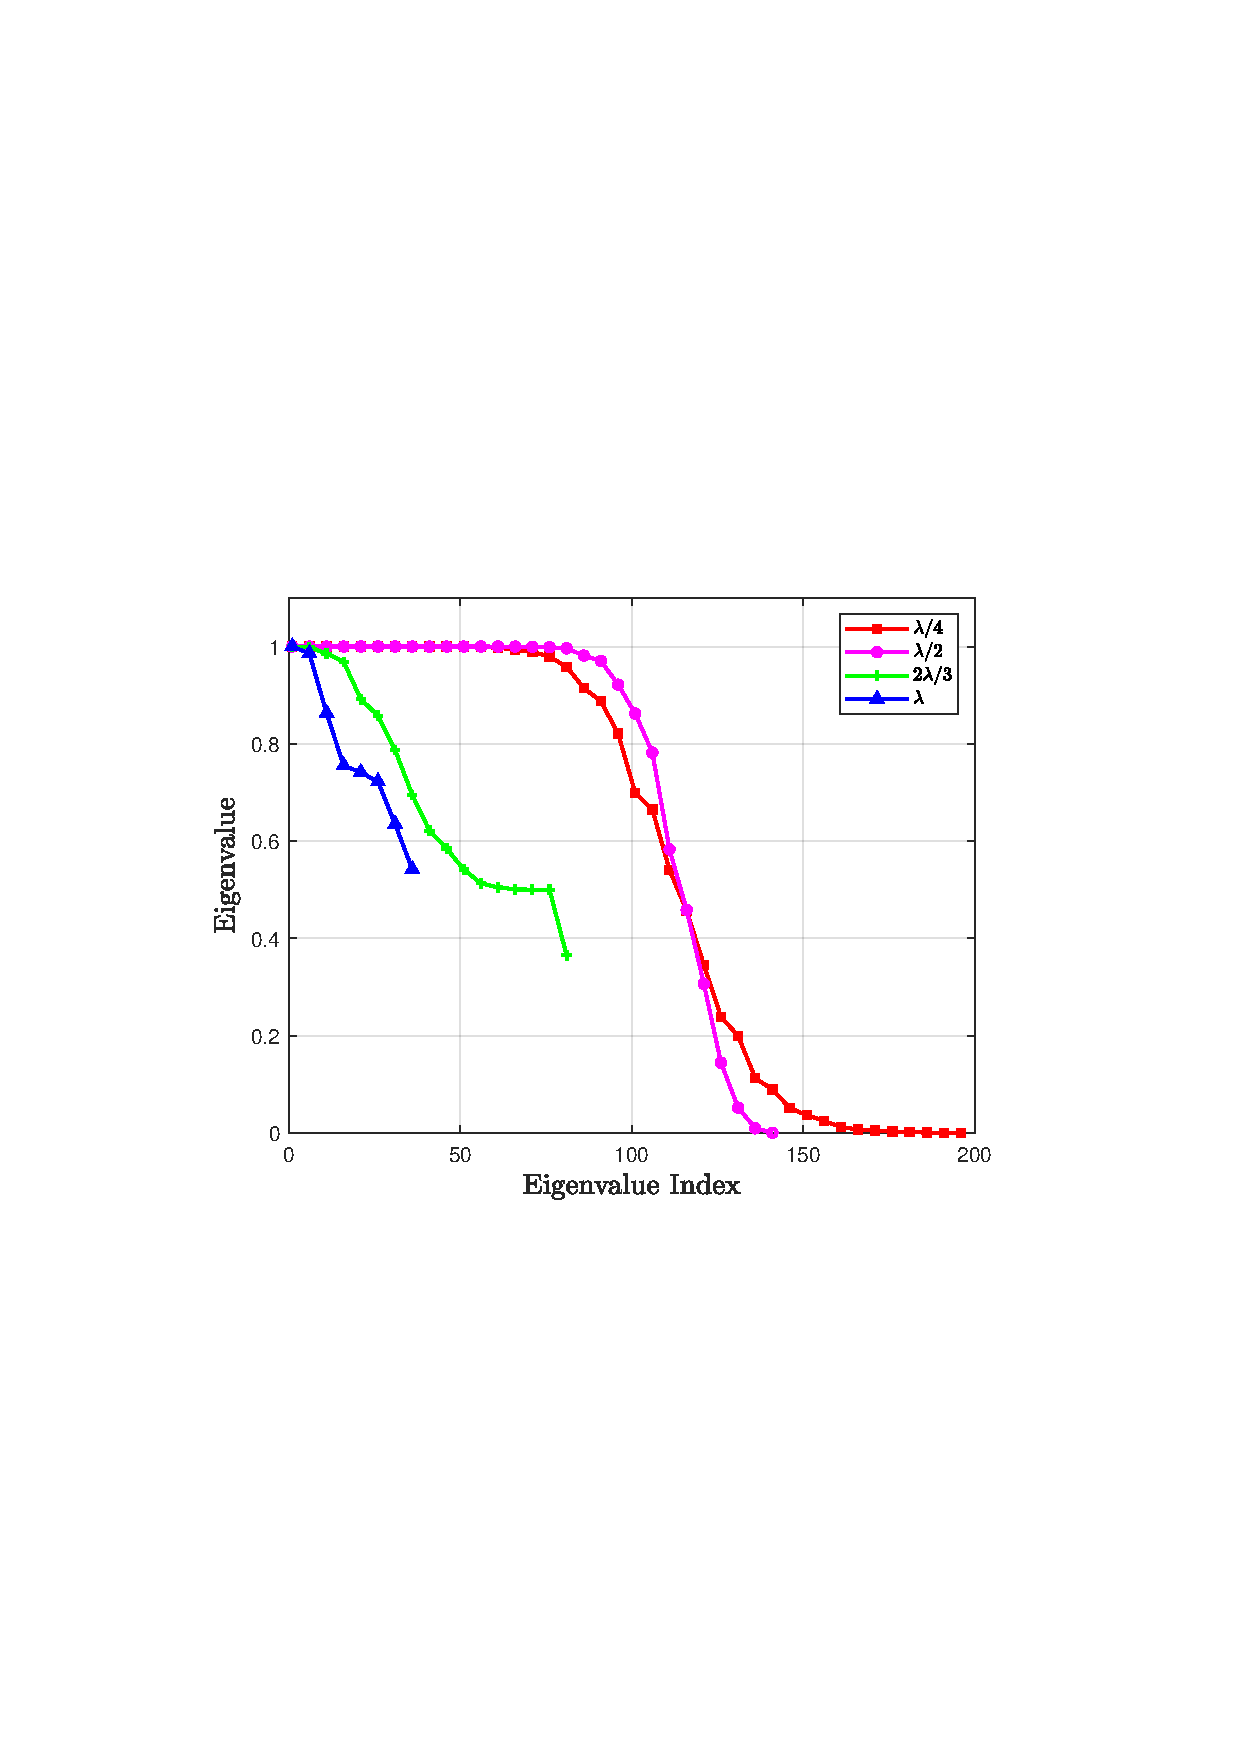
\includegraphics[width=0.7\textwidth]{figs/eigen_two_dimensional.pdf} 
		 	\caption{The DoF gain from the ideal two-dimensional Slepian problem. The antenna array is $6\lambda \times 6\lambda$ with different antenna spacing on $x$ and $y$ axes. The frequency is $3\,{\rm GHz}$.} 
		 	\label{different_z_setting_2d}
		 \end{figure}
		 
		 Figure \ref{different_antenna_spacing_merge} depicts the eigenvalues corresponding to the three-dimensional Slepian concentration problem, where no dimensions of the electromagnetic field's spatial and wavenumber domains are neglected. The size of spatial concentration region is $6\lambda \times 6\lambda \times 2.5\lambda$. To facilitate comparison with the two-dimensional case, the sampling spacing is varied only along the $x$ and $y$ axes, while maintaining half-wavelength sampling along the $z$ axis. It is worth noting that the two-dimensional projection of this three-dimensional array on the $xOy$ plane is consistent with the scenario in Figure \ref{different_z_setting_2d}. According to the conclusions from the previous figure, the characteristics of different sampling spacing on the $x$ and $y$ axes should only be related to the highest frequency and not to the bandwidth, achieving near-optimal results at the half-wavelength sampling. In figure \ref{different_antenna_spacing_merge} we have two different scenarios: broad-band and single-frequency point, both with a highest frequency of $3\,{\rm GHz}$. The broad-band scenario covers $[0,3]\,{\rm GHz}$, corresponding to a solid sphere in the wavenumber concentration region, while the single-frequency point corresponds to a sphere surface in the wavenumber concentration region. It is shown that the characteristics of different sampling spacing differ between the two scenarios. For the broad-band scenario, half-wavelength spacing is necessary, similar to the simulation results of the two-dimensional model. However, for the single-frequency point scenario, about one-third of the eigenvalues tend to zero at half-wavelength spacing, which means that half-wavelength spacing is oversampling. On the contrary, at $2\lambda/3$ spacing, almost all eigenvalues are significantly greater than zero, suggesting that the near-optimal sampling density is around $2\lambda/3$ spacing, which is sparser than half-wavelength sampling. Therefore, for electromagnetic fields in three-dimensional space and wavenumber domain, the near-optimal sampling spacing depends on the structure of the frequency and wavenumber concentration regions, not just the highest frequency. When only considering the two-dimensional problem, the structure of the frequency and wavenumber concentration regions is lost, leading to less accurate results.

		 {\color{red}
\begin{remark}
	(Connection between antenna spacing and eigenvalues) Here, we discuss the relationship between the antenna spacing and eigenvalues from two perspectives. The first perspective concerns the approximation process in numerical computation. The point at which the number of non-zero eigenvalues tends to stabilize, without further significant growth as the discretization order increases, indicates that the performance of the spatial sampling has become close to that of the continuous case. The second perspective concerns the limiting DoF obtained through this approximation. When considering antenna spacing, the model corresponds to using delta functions as basis functions to represent the band-limited fields, instead of the eigenfunctions solved from the concentration problem. From a qualitative standpoint, the required discretization order, which relates to the optimal antenna spacing, is comparable to the number of non-zero eigenvalues. For a specific channel condition, the optimal antenna spacing relates to $cDoF$, while for all possible kinds of channel conditions, the optimal antenna spacing relates to $fDoF$. 
	However, since the basis using delta functions is not the optimal one provided by the concentration problem, a slightly larger number of basis functions may be needed to achieve the same approximation performance. 
\end{remark}
		 }
	

\begin{figure}
	\centering 
	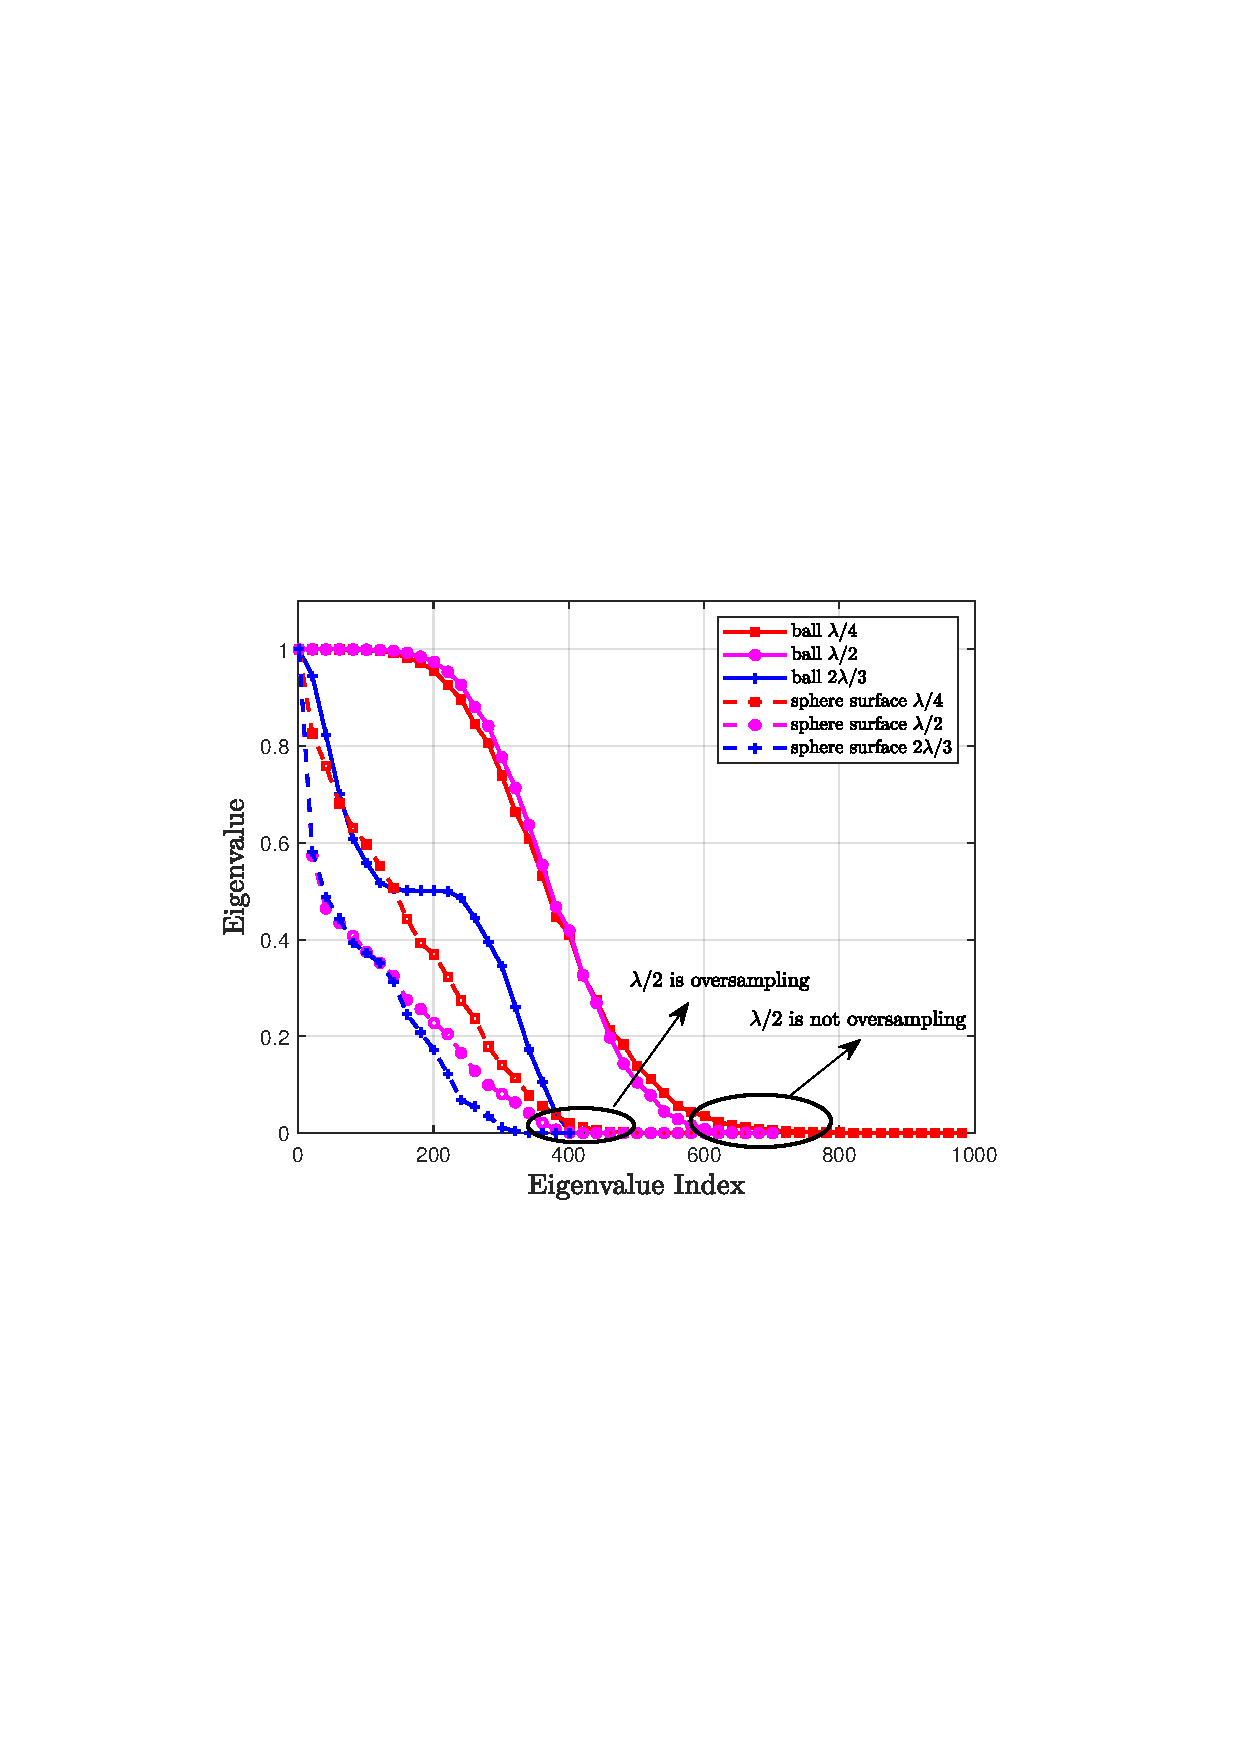
\includegraphics[width=0.7\textwidth]{figs/different_antenna_spacing_merge.pdf} 
	\caption{The DoF gain with different antenna spacing. The 3d-antenna array is $6\lambda \times 6\lambda \times 2.5\lambda$ with different antenna spacing on $x$ and $y$ axes, and $\lambda/2$ antenna spacing on $z$ axis. The frequency is $3\,{\rm GHz}$.} 
	\label{different_antenna_spacing_merge}
\end{figure}

		Moreover, we will discuss the influence of spatial sampling scheme, which corresponds to the spacing between different antennas. In Fig. \ref{different_sampling_scheme_merge} we use both equal antenna spacing and unequal antenna spacing based on Gauss-Legendre quadrature rule. The sampling points and weights of Gauss-Legendre quadrature rule rely on the following Legendre polynomials
		$P_0(x) :=  1$ and
		$P_n(x) := \frac{1}{2^n n!}\frac{{\rm d}^n}{{\rm d}x^n}\left[ (x^2-1)^n \right]$. The sampling points $x_1,\dots,x_n$ are zeros of $P_{n}(x)$, and the weights $A_1,\cdots,A_n$ satisfy
		\begin{equation}
			\begin{aligned}
				A_k = \frac{2}{n} \frac{1}{P_{n-1}(x_k)P^{'}_{n}(x_k)}.
			\end{aligned}
		\end{equation}
		It is obvious that unequal antenna spacing does not change the number of non-zero eigenvalues, which means that the DoF will not be greatly influenced and converge to the same upperbound determined by continuous aperture. However, unequal antenna spacing influences the decay rate of eigenvalues. In our simulation results, Gauss-Legendre sampling scheme corresponds to more large eigenvalues compared to classical equal sampling scheme. This phenomenon may be used when we need to design limited number of electromagnetic patterns to convey information. With Gauss-Legendre sampling scheme we can have a better approximation to expected electromagnetic fields with a fixed number of patterns, and use fewer patterns for given approximation accuracy to expected electromagnetic fields.

\begin{figure}
	\centering 
	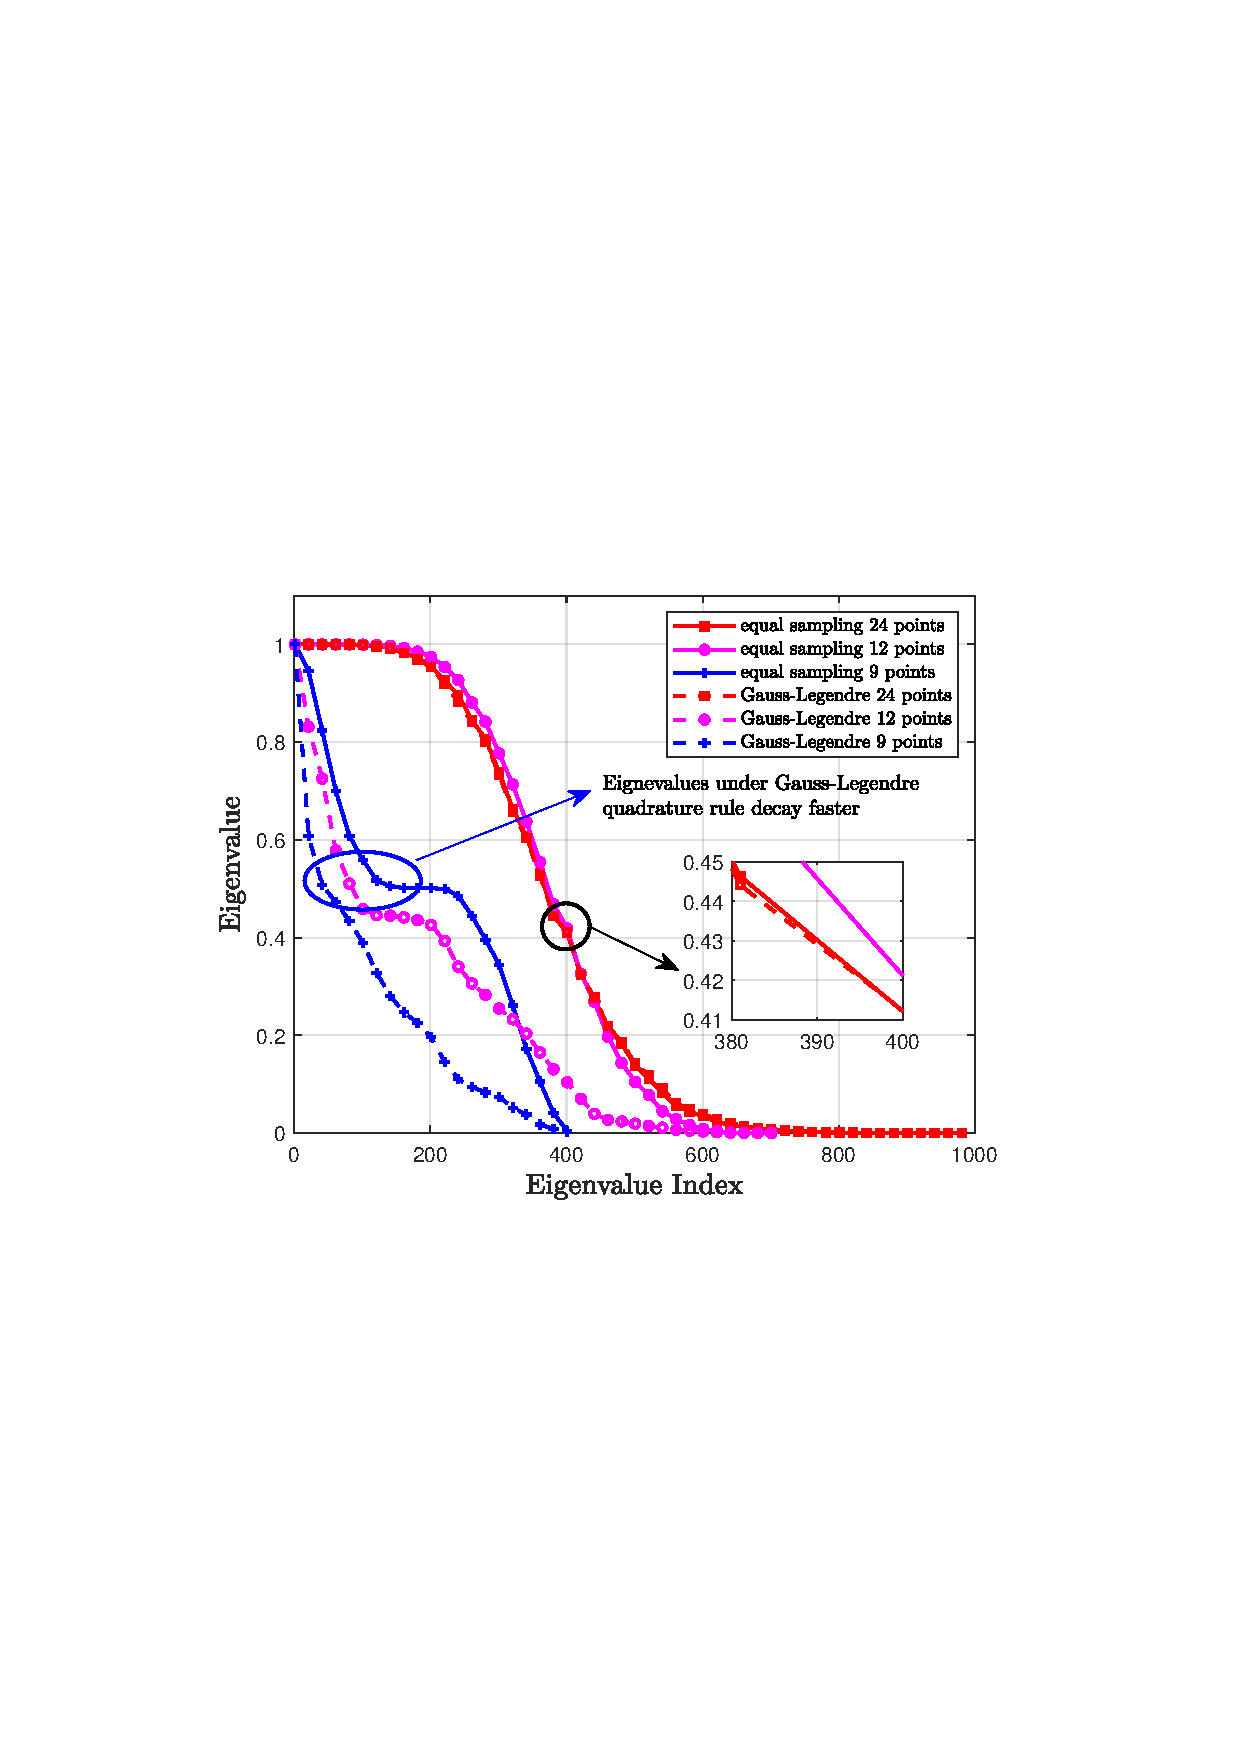
\includegraphics[width=0.7\textwidth]{figs/different_sampling_scheme_merge.pdf} 
	\caption{The DoF gain with different sampling points with equal sampling and Gauss-Legendre quadrature rule. The 3d-antenna array is $6\lambda \times 6\lambda \times 2.5\lambda$ with different sampling points on $x$ and $y$ axes, and $\lambda/2$ antenna spacing on $z$ axis. The frequency band is $[0,3]\,{\rm GHz}$.} 
	\label{different_sampling_scheme_merge}
\end{figure}

Finally we consider both the space and time domains to provide more general results for electromagnetic information theory. Noted that for wireless communication systems the time-harmonic assumption requires the periodicity of the electromagnetic field in the time domain, that is, the theoretical model is strictly satisfied only after the electromagnetic field becomes stationary. The above communication process will greatly reduce the efficiency of wireless communication and is not practical enough. Therefore, without the time-harmonic assumption, we can obtain a more general model for electromagnetic information theory, which better fits practical wireless communication processes. With the theoretical analysis, we plot the space-time patterns inspired by Slepian concentration problem in Fig. \ref{fig_cdl_fit}. For ease of calculation, we bound the electromagnetic fields on one-dimensional space domain which corresponds to linear antenna array. These patterns have good orthogonality, shown in Fig. \ref{pattern_correlation}. Moreover, according to \eqref{eqn_min_f_approx} we know that these patterns can be used to construct arbitrary required electromagnetic fields in the source/destination regions with a given approximation error. {\color{red} We can also observe that eigenfunctions that vary slower on the space domain correspond to larger eigenvalues, which fits our previous analysis.}

	\begin{figure}[!t]
	\setlength{\abovecaptionskip}{-0.0cm}
	\setlength{\belowcaptionskip}{-0.0cm}
	\centering
	\subfigcapskip -0.5em
	\subfigure[Pattern 1]{
		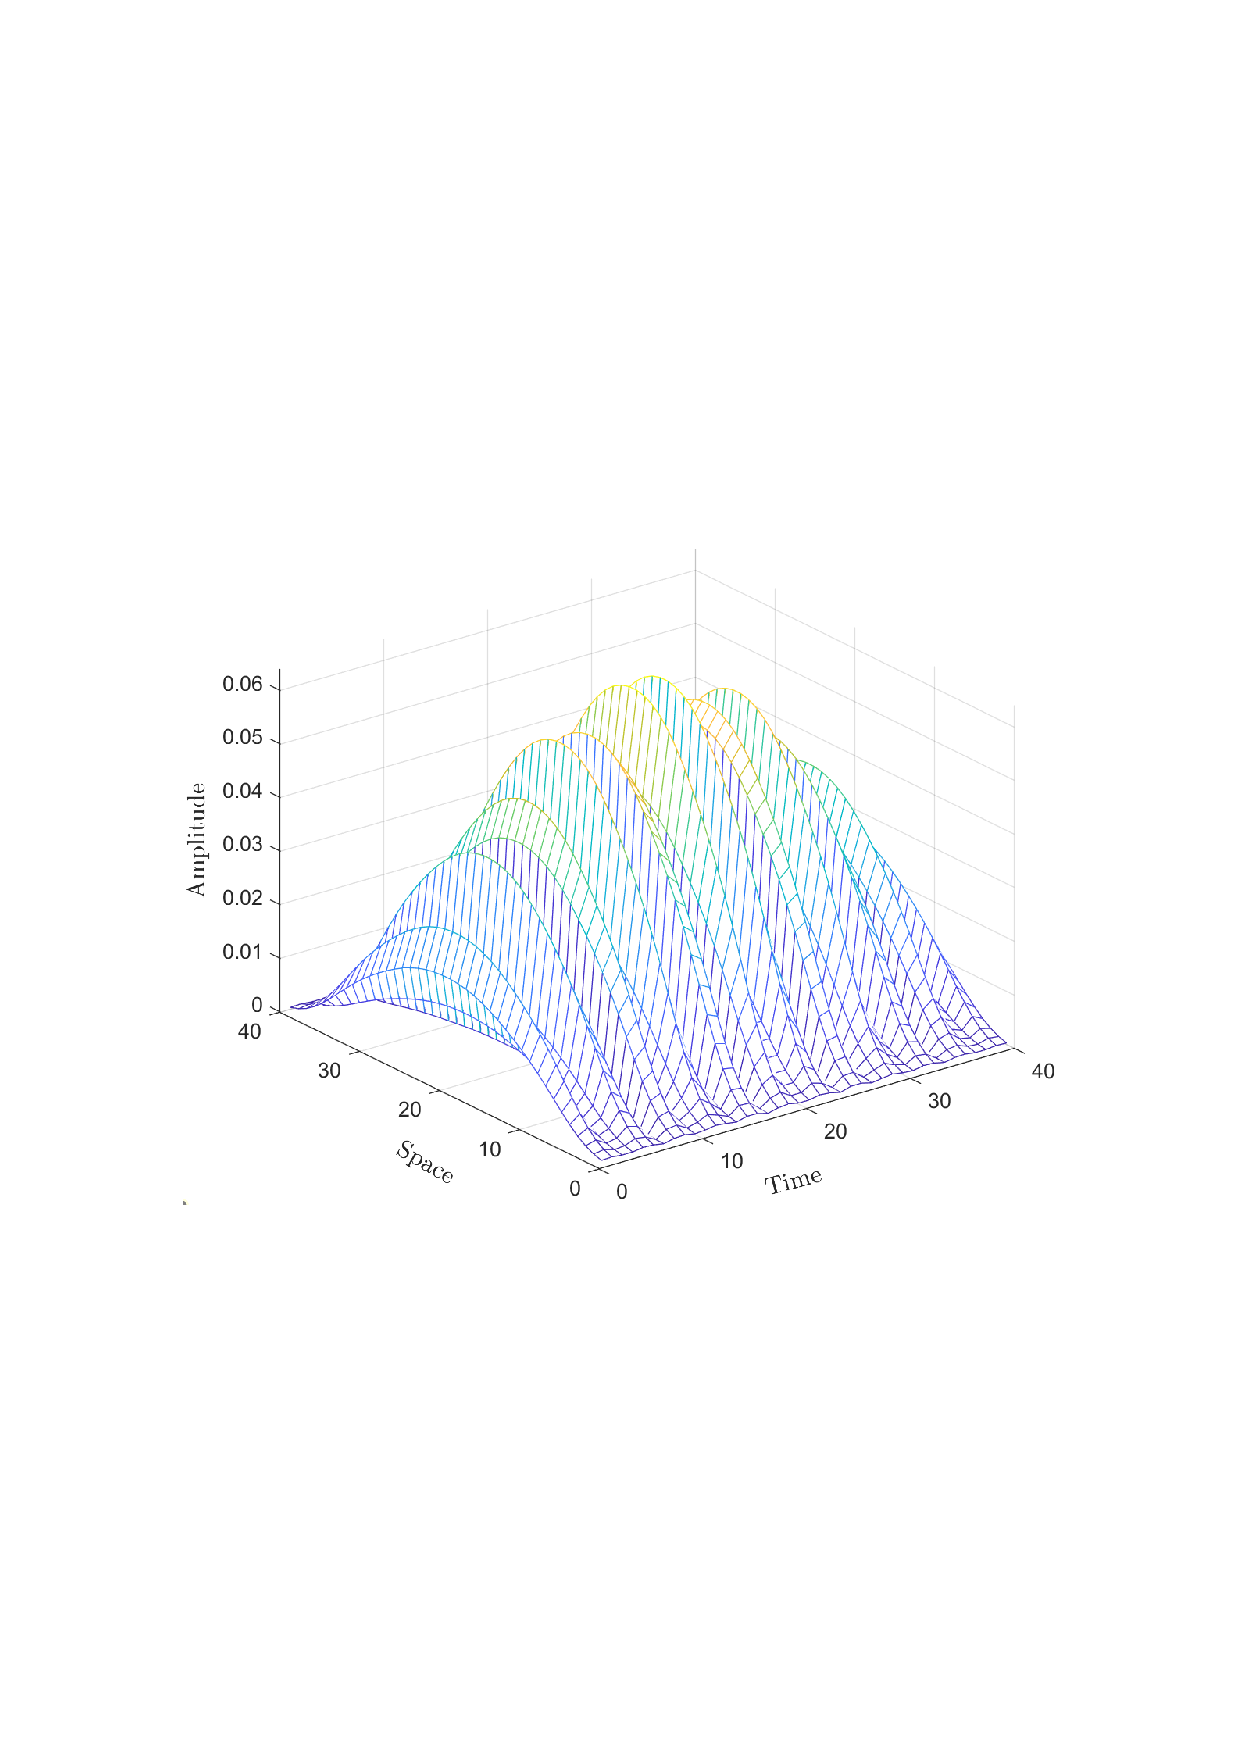
\includegraphics[width=3in]{figs/eigf1.pdf}
	}%\hspace{-2em}
	\subfigure[Pattern 2]{
		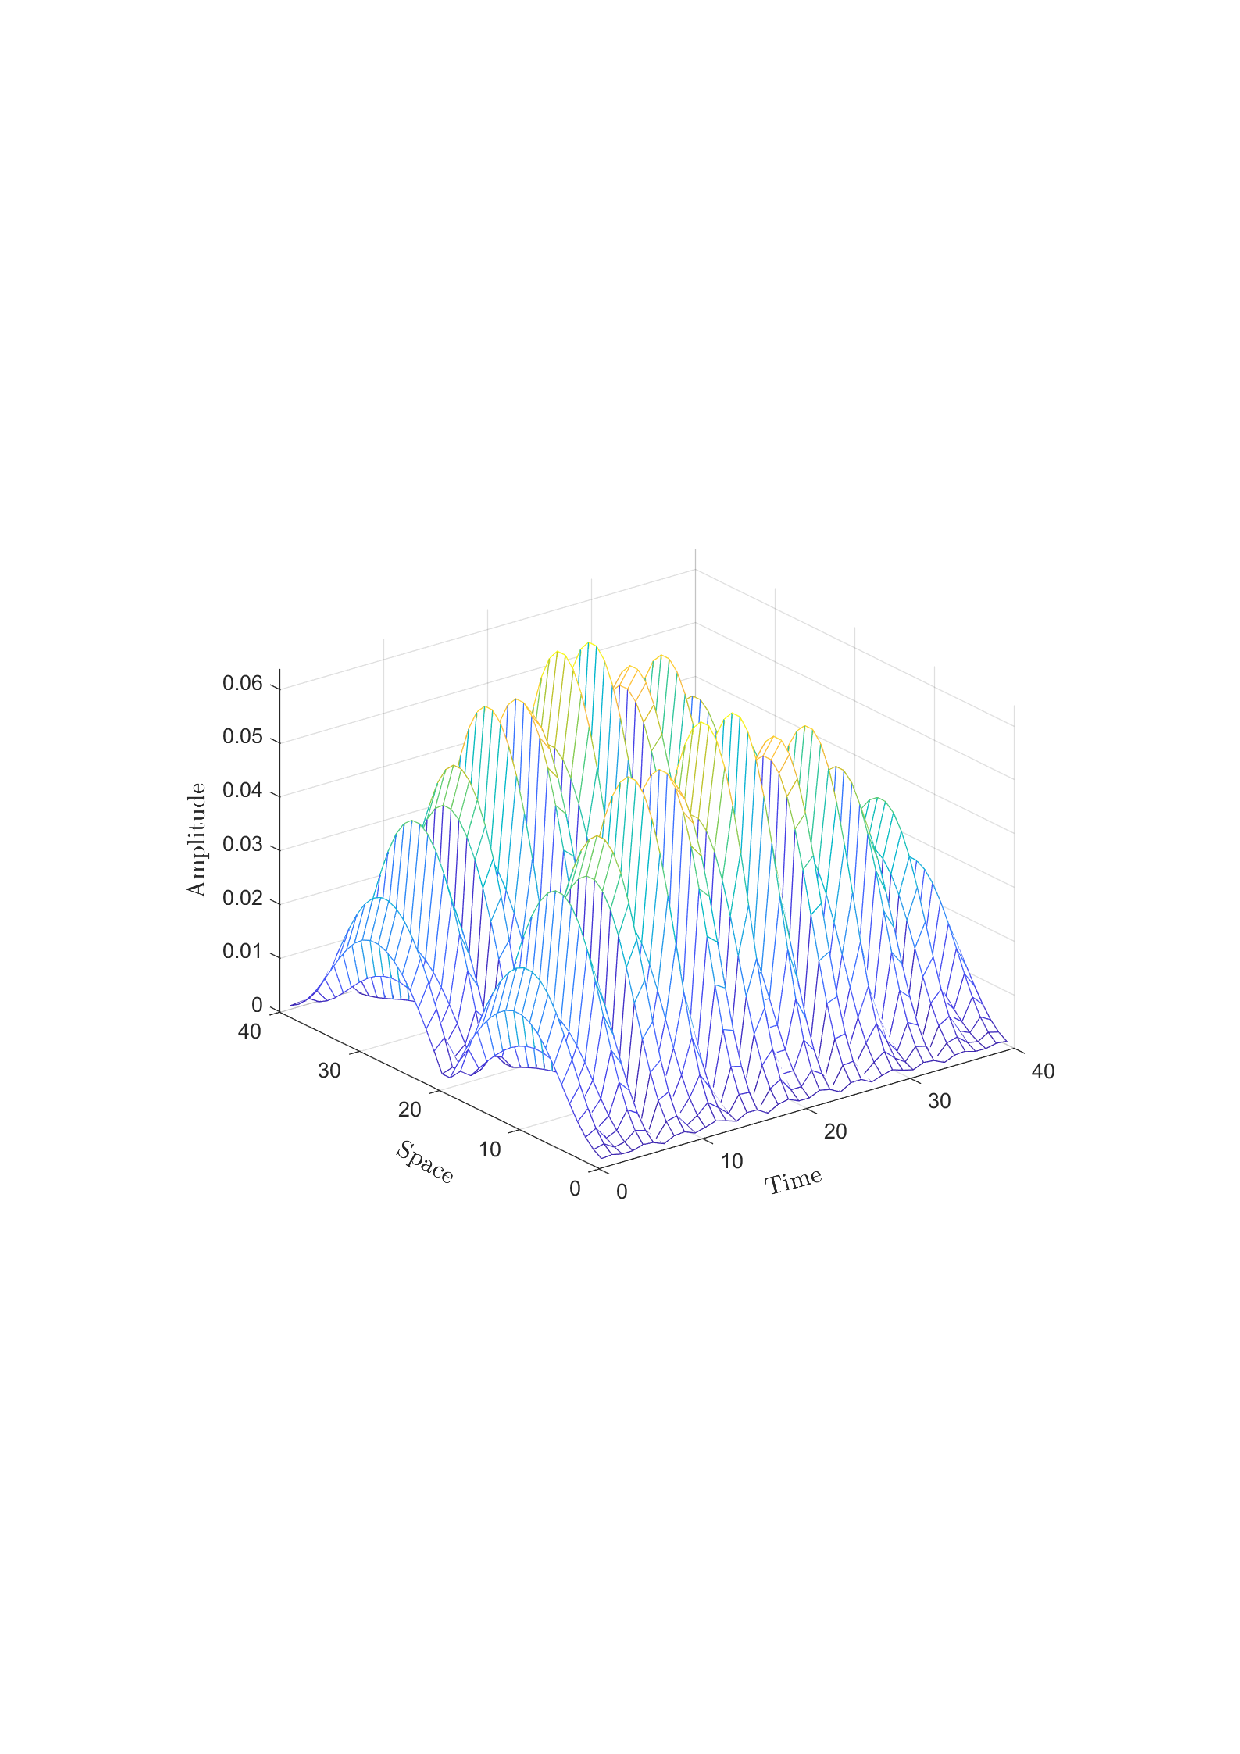
\includegraphics[width=3in]{figs/eigf2.pdf}
	}
	
	\subfigure[Pattern 3]{
		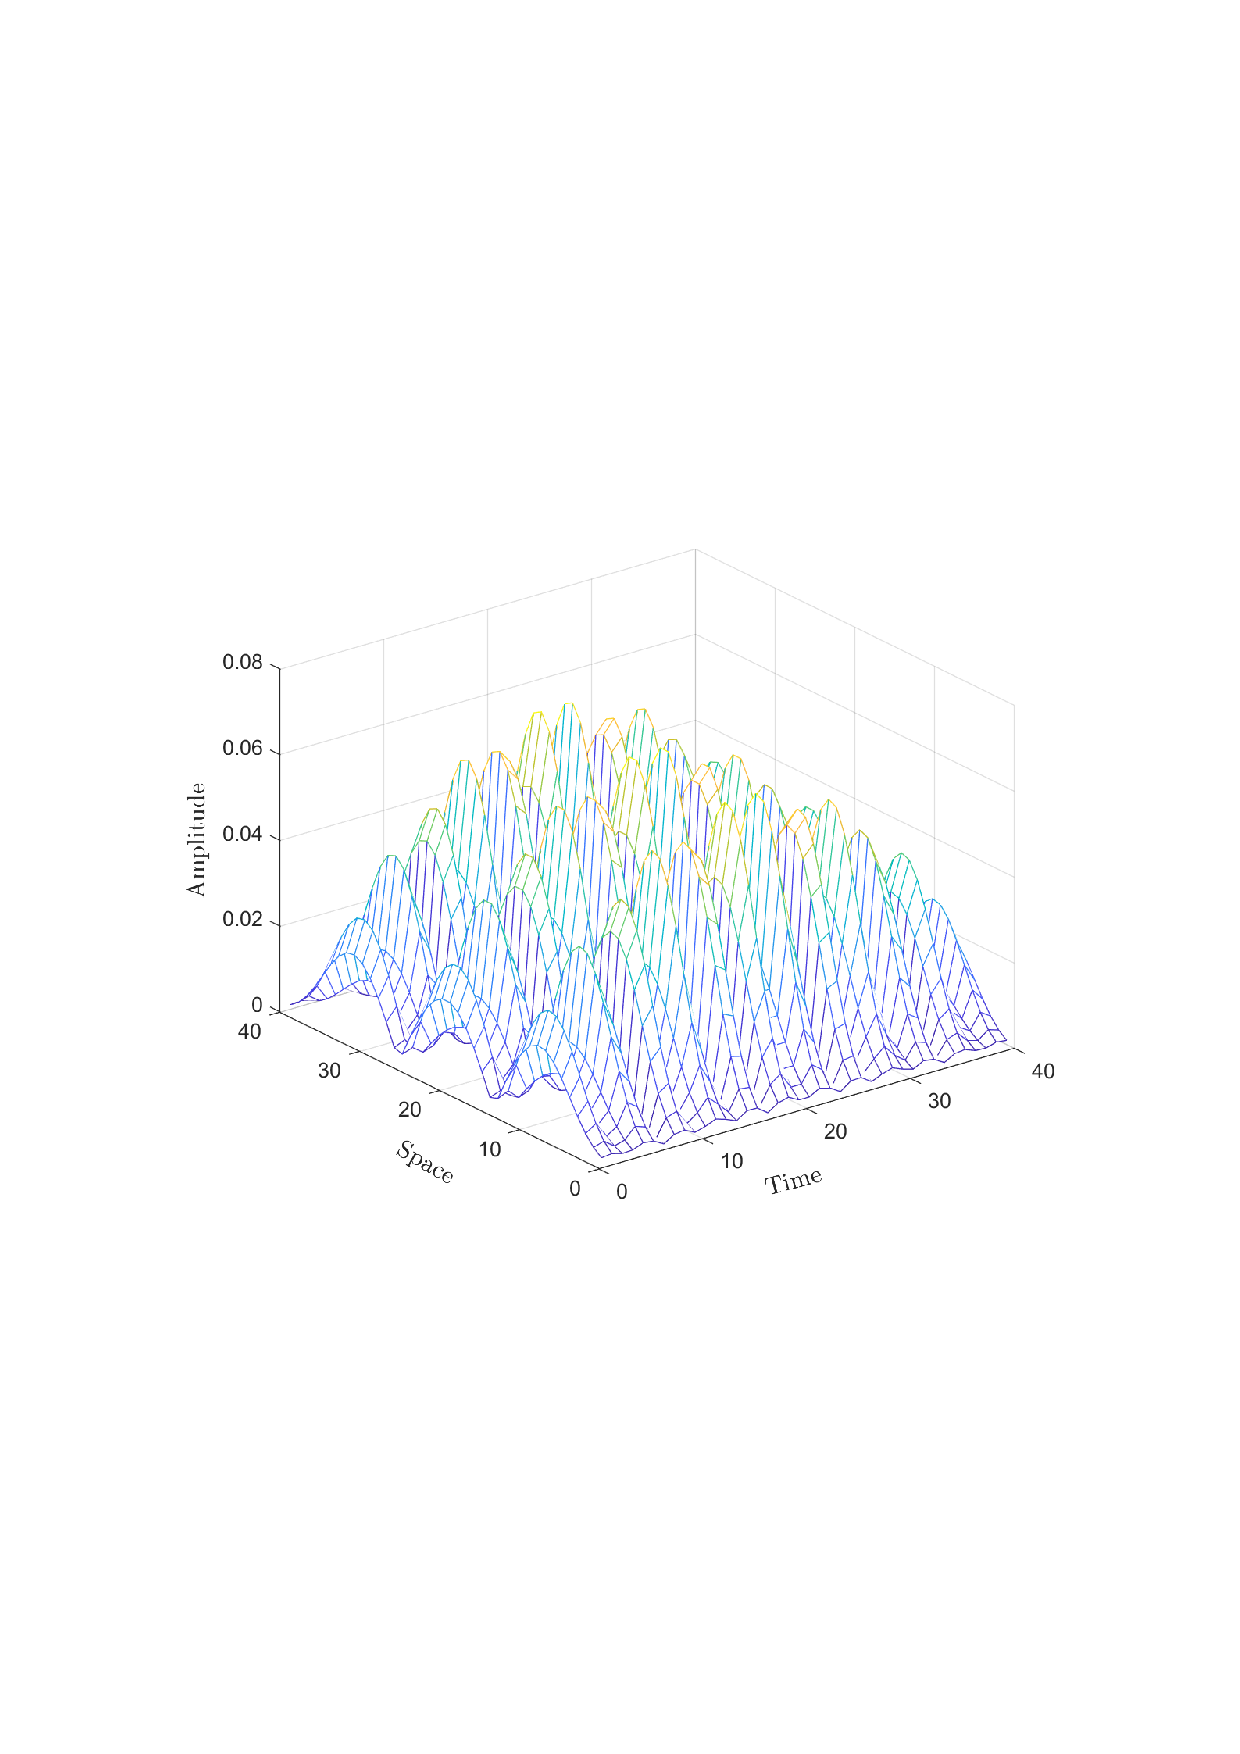
\includegraphics[width=3in]{figs/eigf3.pdf}
	}%\hspace{-2em}
	\subfigure[Pattern 4]{
		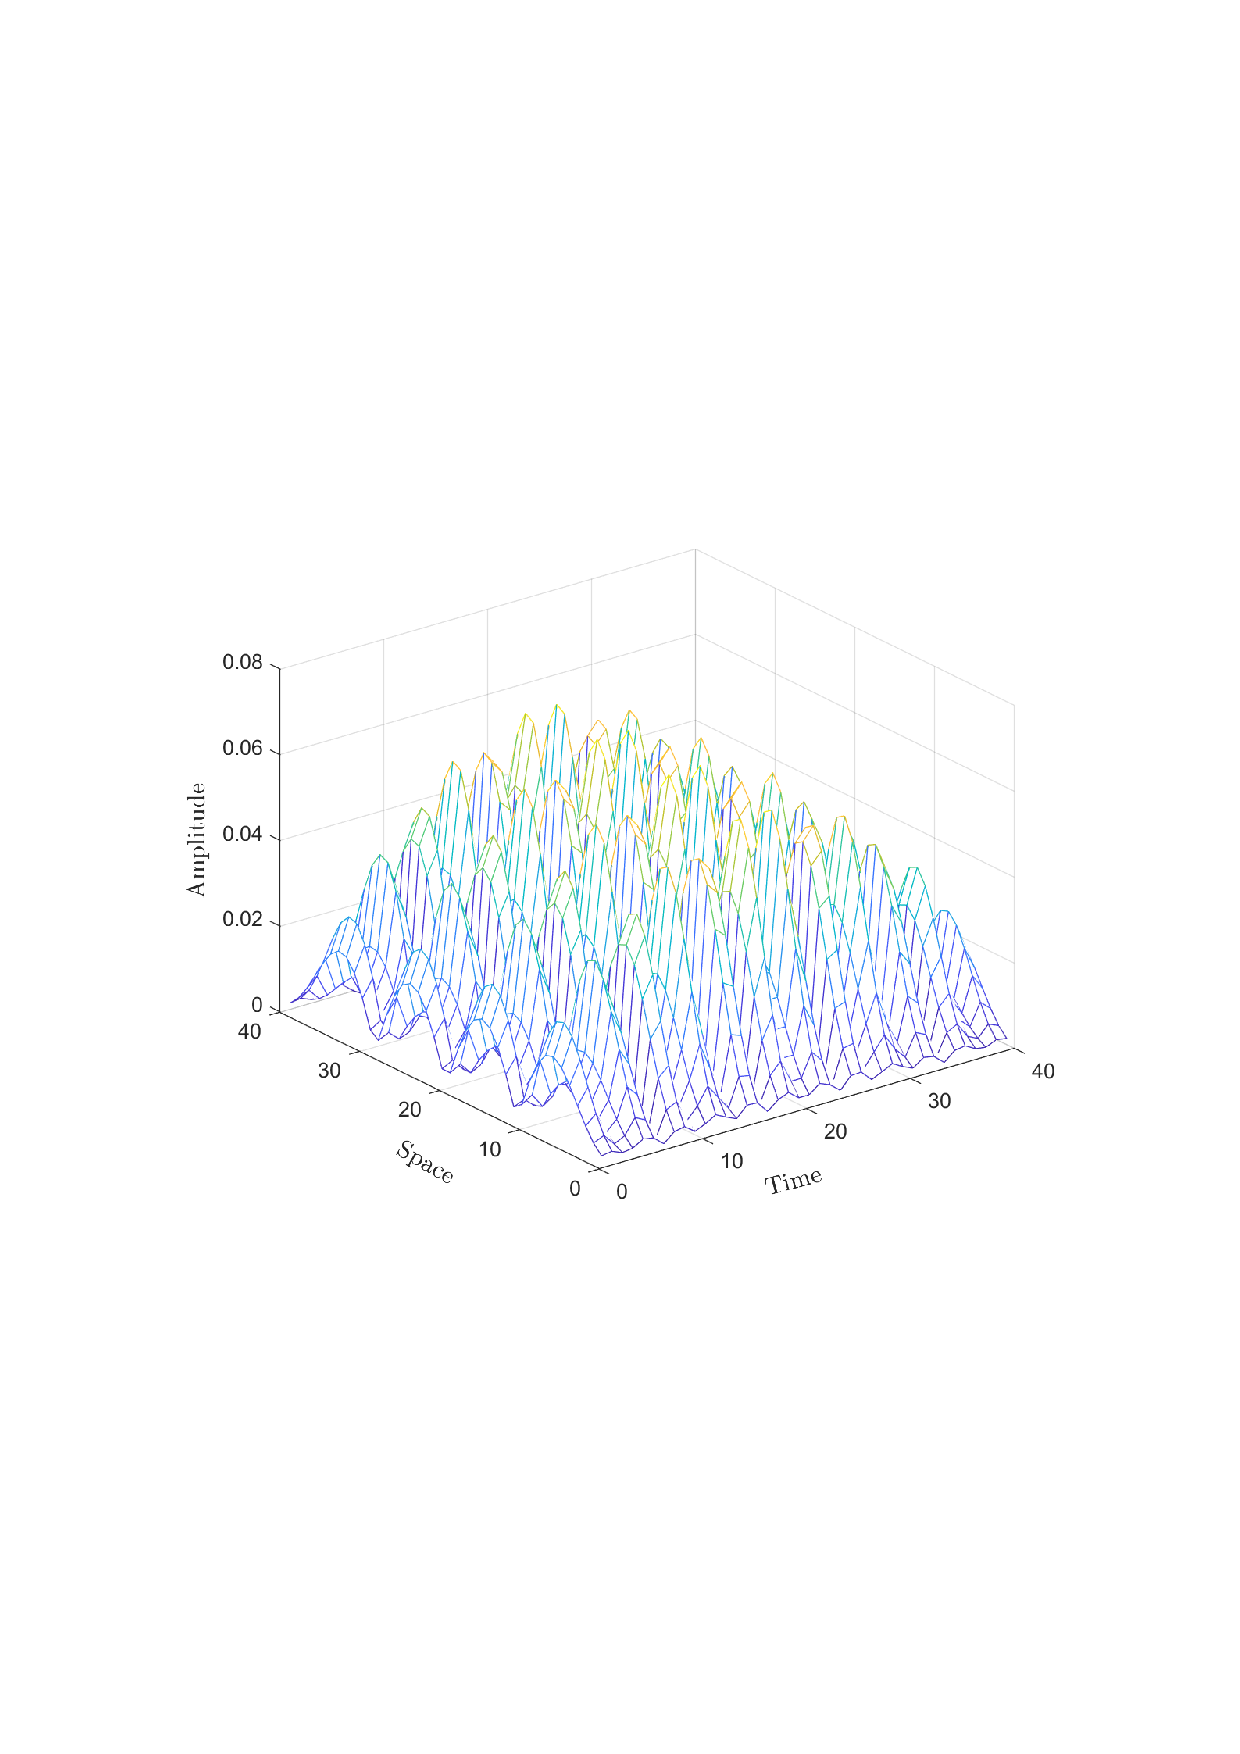
\includegraphics[width=3in]{figs/eigf4.pdf}
	}
	
	\subfigure[Pattern 5]{
		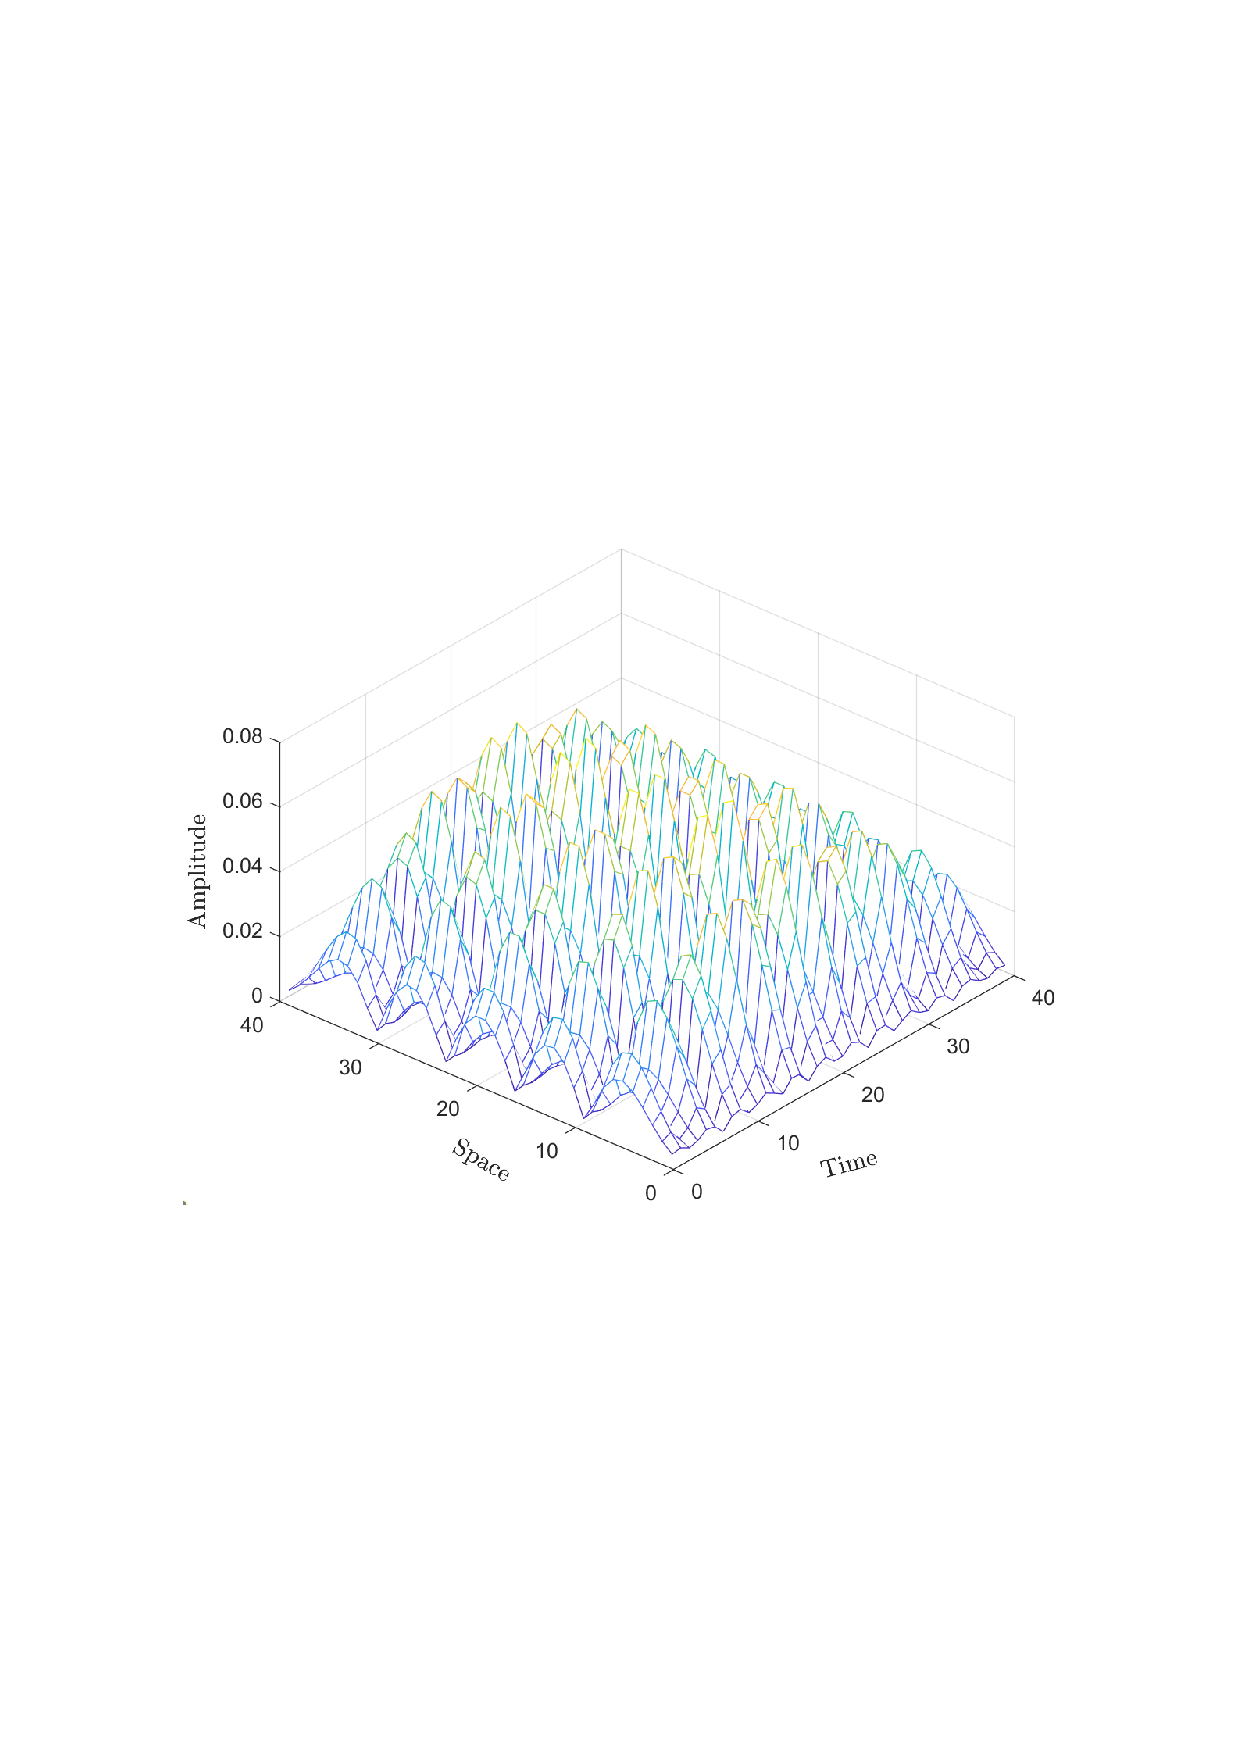
\includegraphics[width=3in]{figs/eigf5.pdf}
	}%\hspace{-2em}
	\subfigure[Pattern 6]{
		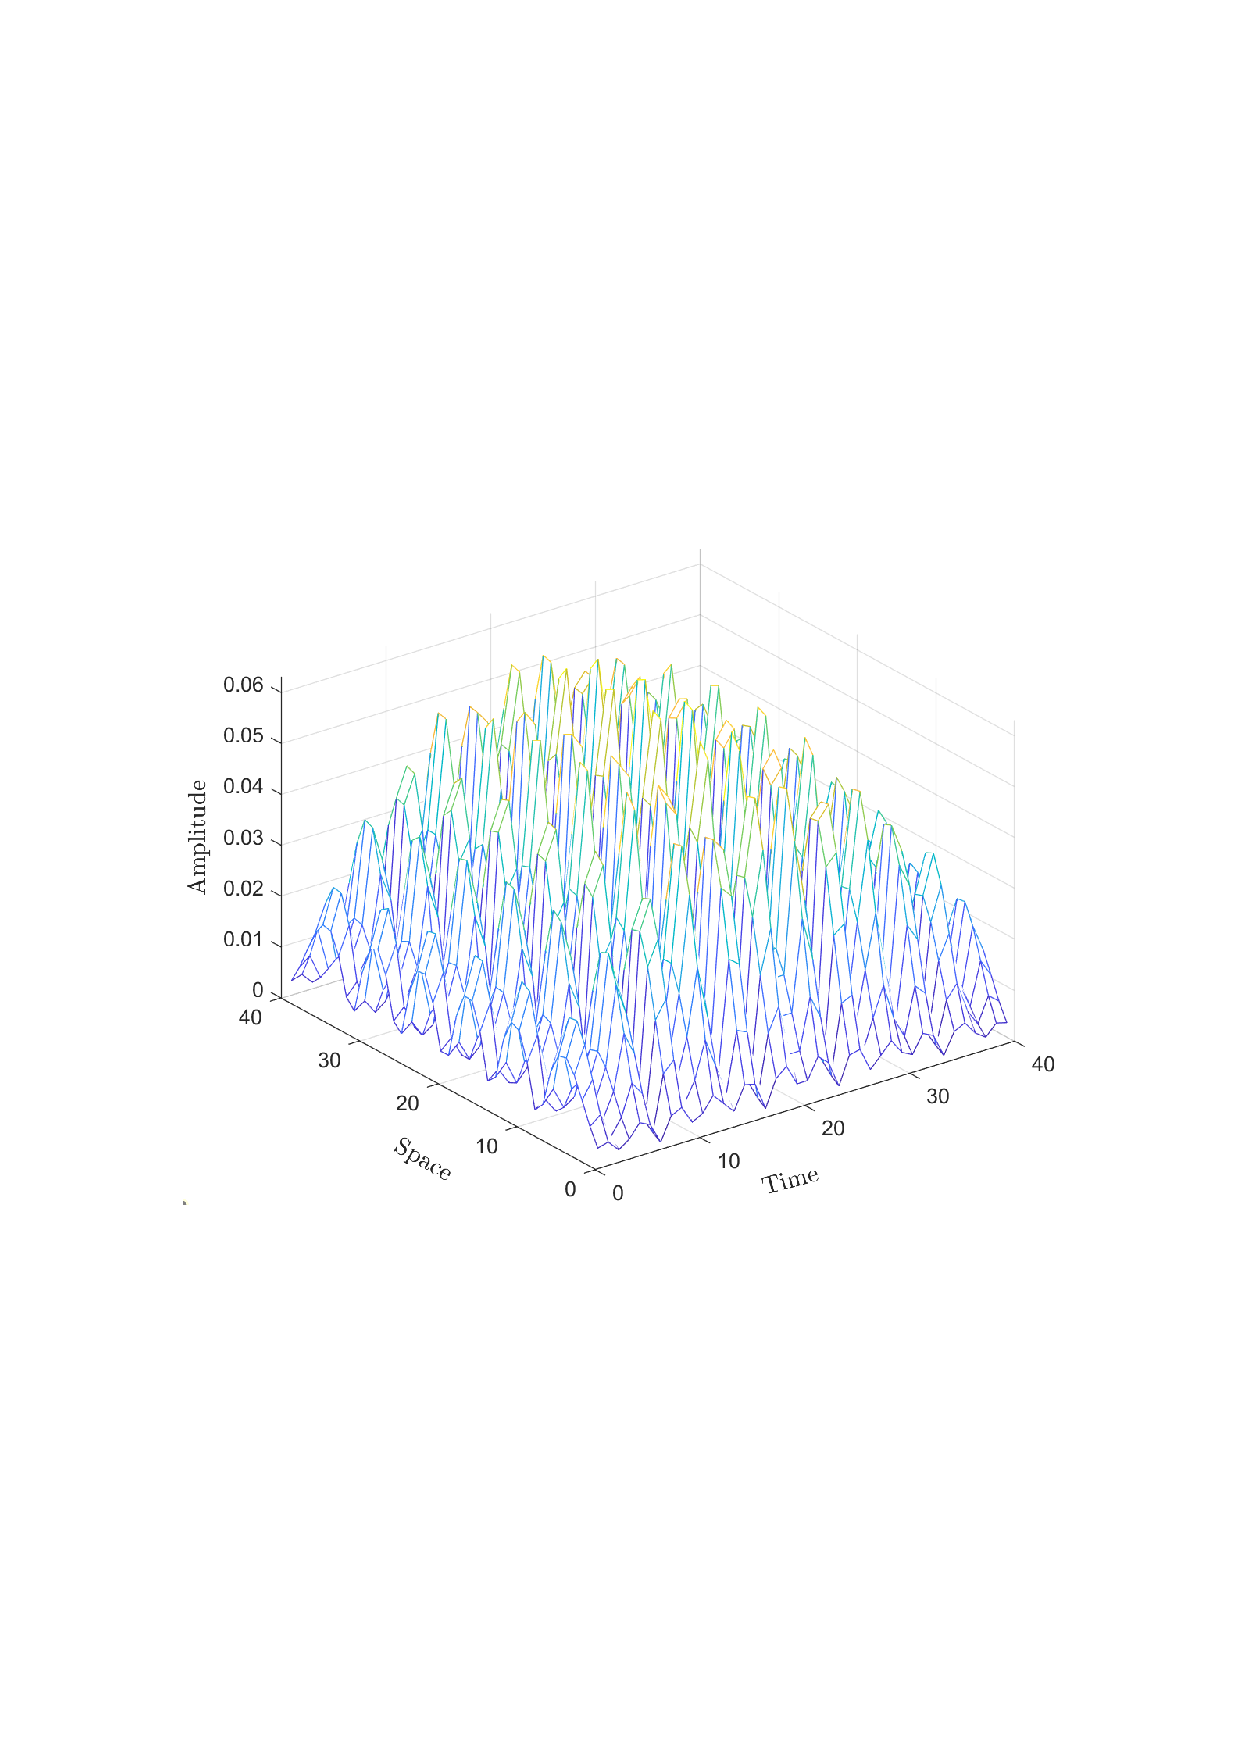
\includegraphics[width=3in]{figs/eigf6.pdf}
	}
	
	%\hspace{-2em}
	%\vspace{1em}
	\caption{
		The first 6 orthogonal space-time patterns that satisfy the electromagnetic constraints and concentrate in the observation region. 
	}
	%\vspace{-1em}
	\label{fig_cdl_fit}
\end{figure}

\begin{figure}
	\centering 
	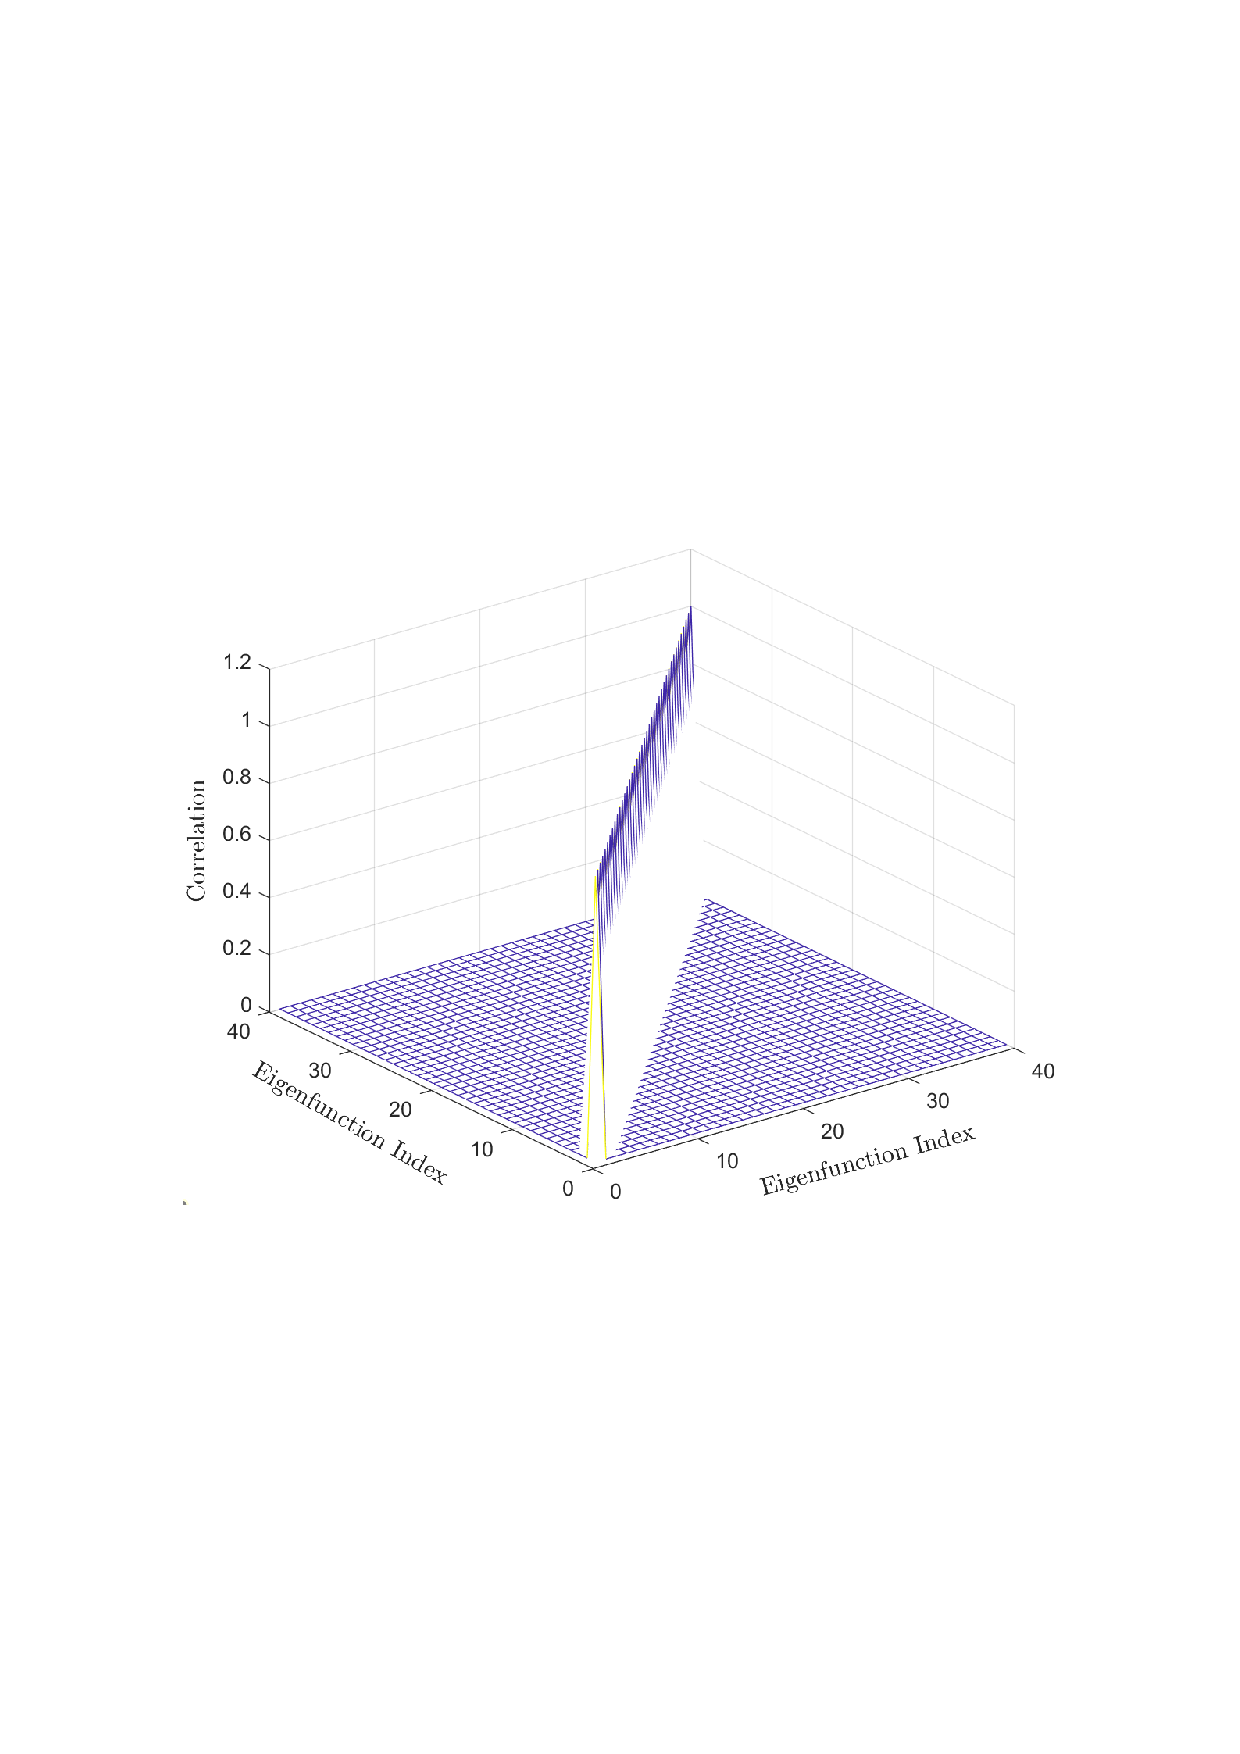
\includegraphics[width=0.7\textwidth]{figs/eigen_function_correlation.pdf} 
	\caption{The correlation of the space-time patterns.} 
	\label{pattern_correlation}
\end{figure}

\section{Conclusion}
In this paper, we provide a general DoF and pattern analyzing scheme for EIT. {\color{red}Specifically, we begin from electromagnetic models and provide mathematical definitions of functional DoF and channel DoF of continuous electromagnetic fields. Based on the mathematical definitions, we theoretically discuss the relationship between them.
Then, we extend the classical Slepian concentration problem to the three-dimensional space domain and the four-dimensional space-time domain to obtain the DoF of the electromagnetic fields with given physical constraints.} Finally, we provide numerical simulations to verify the theoretical analysis and show more insights, including the near-optimal spatial sampling interval of antenna array, the DoF of three-dimensional antenna array, the impact of unequal antenna spacing, the orthogonal space-time patterns, etc. For example, our simulation results show that with a narrow frequency bandwidth, half-wavelength antenna spacing may not be necessary to achieve the DoF upperbound.

Further research work can be focused on deriving analytical expressions of eigenvalues and eigenfunctions instead of numerical simulations in some specific cases. Moreover, a tighter bound between functional DoF and channel DoF is expected.

\section*{Acknowledgment}

The authors sincerely thank Prof. Lizhong Zheng and Prof. Husheng Li for their valuable comments on this work.

	
	\footnotesize
	
	\bibliographystyle{IEEEtran}
	%\clearpage
	
	\bibliography{bib}
\end{document}